\section{Expected exit time from a domain}
We aim to estimate the exit time of a particle driven by a deterministic transport field and a stochastic diffusion from a domain $D \subset \mathbb{R}^d$. Given a vector $W(t)$ of $m$ independent Brownian motions and two functions $f\colon \mathbb{R}^d \rightarrow \mathbb{R}^d, g \colon \mathbb{R}^d \rightarrow \mathbb{R}^{d\times m}$, we consider the following stochastic differential equation (SDE)
\begin{equation}\label{eq:GeneralModel}
\begin{cases}
	dX(t) = f(X(t)) dt + g(X(t))dW(t), & 0 < t \leq T, \\
	X(0)  = X_0, & X_0 \in D.
\end{cases}
\end{equation}
The problem is completed with two different types of boundary conditions, namely
\begin{itemize}
	\item[i.]  \textit{killing boundaries}: if the particle exits $D$ the process is stopped,
	\item[ii.] \textit{reflecting boundaries}: the particle trajectory is reflected normally inside $D$ when it touches the boundary $\partial D$.
\end{itemize}
Our aim is to estimate numerically the first exit time of the solution $X(t)$ from $D$, \textit{i.e.}, the quantity
\begin{equation}\label{eq:GeneralTau}
	\tau = \min\{\min\{t\colon X(t)\notin D\},T\}.
\end{equation}
Let us remark that the parameter $\tau$ is meaningful only if there exists a portion of the boundary $\Gamma_k \subset \partial D$ that is endowed with killing boundary conditions. Otherwise, the process $X(t)$ will stay in $D$ for the whole time interval, giving as a result $\tau = T$ for each realisation of $X(t)$. Another quantity of interest is defined as follows
\begin{equation}\label{eq:GeneralPhi}
	\phi = \phi(T,X_0,F) = \mathbbm{1}_{\{\tau<T\}}F(X(T)),
\end{equation}
where $F\colon \mathbb{R}^d \rightarrow \mathbb{R}$ is a smooth function. An interesting choice of $F$ could be the function mapping every $x$ of $\mathbb{R}^d$ to the value 1, thus giving as a result for $\phi$ the probability for $X(t)$ to exit the domain before the final time $T$. Let us choose the notation $F = 1$ in this case, getting
\begin{equation}\label{eq:ExitProb}
	\Phi(T,X_0) = \phi(T,X_0,1) = \Pr(\tau < T | X(0) = X_0)
\end{equation}
In the case of general $f,g$ and for a $d$-dimensional SDE, there is no closed form for $\tau$ and $\phi$. Therefore, we approximate the value of $\tau$ by means of two numerical schemes, briefly presented in the following.
\begin{frame}[plain]
\frametitle{Discrete Euler-Maruyama}
Method:
\begin{equation*}
	\left \{
	\begin{aligned}
		X_h^d(t_{i+1}) &= f(X(t_i))h + g(X(t_i))(W(t_{i+1}) - W(t_{i})),  \\
		X_h^d(0) &= X_0.
	\end{aligned} \right .
\end{equation*}
Parameters of interest computed naively
\begin{equation*}
\begin{aligned}
	\tau_h^d &= \min\{\tau_{h,e}^d,T\}, \text{ where } \tau_{h,e}^d = \min \{t_i \colon X_h^d(t_i) \notin D\}, \\
	\phi_h^d &= \mathbbm{1}_{\{T < \tau_{h,e}^d\}}F(X_h^d(T)).
\end{aligned}
\end{equation*}
Missed exits $\Rightarrow$ 1/2 loss in weak order:
\begin{align*}
	|\mathbb{E}(\tau_h^d) - \mathbb{E}(\tau)| &= O(\sqrt{h}), \\
	|\mathbb{E}(\phi_h^d) - \mathbb{E}(\phi)| &= O(\sqrt{h}).
\end{align*}	
\end{frame}

\begin{frame}[plain]
\frametitle{Continuous Euler-Maruyama}
\underline{Goal}. Restore the order of convergence 1 of Euler-Maruyama in $\R^d$ $\Rightarrow$ Brownian bridge approach.

Method:
\begin{equation*}
	\left \{
	\begin{aligned}
		X_h^c(t) &= f(X(t_i))(t-t_i) + g(X(t_i))(W(t) - W(t_{i})),  && t_i < t \leq t_{i+1},\\
		X_h^c(0) &= X_0.
	\end{aligned} \right .
\end{equation*} 
Estimate at each time step the probability of exit. If $D$ is an half-space
\begin{equation*}
\begin{aligned}
	&\Pr (\exists t \in [ t_i,t_{i+1} ] \quad X_h^d(t) \notin D | X_h^d(t_i) = x_i, X_h^d(t_{i+1}) = x_{i+1}) \\
	&\quad = p(x_i,x_{i+1},h) \\
	&\quad = \exp\Big(-2\frac{[n\cdot(x_i - z_i)][n\cdot(x_{i+1} - z_i)]}{hn\cdot (gg^T(x_i)n)}\Big),
\end{aligned}
\end{equation*}
\end{frame}

\begin{frame}
\frametitle{Continuous Euler-Maruyama}
Parameters of interest. Given $u$ a realization of $U$ uniform r.v. in $(0,1)$
\begin{equation*}
\begin{aligned}
	\tau_h^c &= \min \{T,\tau_{h,e}^c\}, \\
	\text{ where } \tau_{h,e}^c &= \min\{\tau_{h,e1}^c, \tau_{h,e2}^c\}, \\
	\tau_{h,e1}^c &= \min\{t_i = hi \colon X_h(t_i) \notin D\}, \\
	\tau_{h,e2}^c &= \min\{t_i = hi \colon u < p(x_{i-1},x_i,h) \}, \\
	\phi_h^c &= \mathbbm{1}_{\{T < \tau_{h,e}^c\}}F(X_h^c(T)).
\end{aligned}
\end{equation*}
Weak order 1 is restored:
\begin{align*}
	|\mathbb{E}(\tau_h^c) - \mathbb{E}(\tau)| &= O(h), \\
	|\mathbb{E}(\phi_h^c) - \mathbb{E}(\phi)| &= O(h).
\end{align*}
\end{frame}

\subsection{A PDE approach}\label{sec:PDEs}
It is possible to express the mean exit time and the probability of exit from a domain in terms of the solution of partial differential equations (PDE's).
Let us denote by $\Gamma_k,\Gamma_r$ the killing and reflecting subsets of $\partial D$. We consider then the expectation of the exit time from the domain $D$ for a trajectory that at $t=0$ is at position $x$, \textit{i.e.},
\begin{equation}\label{eq:ExpTau}
	\bar\tau(x) = \mathbb{E}(\tau | X(0) = x).
\end{equation}
Let us define the operator $\mathcal L$ induced by \eqref{eq:GeneralModel}, which is applied to a function $u\colon \mathbb{R}^d \rightarrow \mathbb{R}$  as follows
\begin{equation}\label{eq:LOperator}
	\mathcal Lu = f \cdot \nabla u + \frac{1}{2} gg^T : \nabla \nabla u,
\end{equation}
where the $:$ operator between two matrices $A,B$ in $\mathbb{R}^{d\times d}$ is defined as follows
\begin{equation}\label{eq:twoPoints}
	A : B = \sum_{i,j = 1}^d \{A\}_{ij}\{B\}_{ij} = \text{tr}(A^TB).
\end{equation}
The following result allows computing the mean exit time as the solution of an appropriate PDE.

\begin{theorem} Let $\mathcal L$ be the differential operator defined as \eqref{eq:LOperator}. Then, if $\Gamma_k$ and $\Gamma_r$ are respectively the killing and reflecting subsets of $\partial D$, such that $\Gamma_k \cup \Gamma_r = \partial D, \Gamma_k \cap \Gamma_r = \emptyset$, the mean exit time $\bar \tau(x)$ for the solution $X(t)$ of \eqref{eq:GeneralModel} with $X_0 = x$ is the solution of the following boundary value problem
\begin{equation}\label{eq:PDETau}
\left \{
\begin{aligned}
	\mathcal L \bar \tau(x) &= -1, && \text{in } D, \\
	\bar\tau(x) &= 0, && \text{on } \Gamma_k, \\
	\nabla \bar\tau(x) \cdot n &= 0, && \text{on } \Gamma_r,
\end{aligned} \right .
\end{equation}
where $n$ is the normal to $\Gamma_r$.
\end{theorem}
\noindent Further analytic treatment of the mean exit time can be found in \cite{Krumscheid2015,Pavliotis2014}. \\
We now consider the probability of exit from $D$ for a solution $X(t)$ that is equal to $x$ for at a time $s$ smaller than the final time $T$. This probability is the solution of a boundary value problem.
\begin{theorem} Let $\mathcal L$ be the differential operator defined as \eqref{eq:LOperator}. Then, if $\Gamma_k$ and $\Gamma_r$ are respectively the killing and reflecting subsets of $\partial D$, such that $\Gamma_k \cup \Gamma_r = \partial D, \Gamma_k \cap \Gamma_r = \emptyset$
\begin{equation}\label{eq:ExitProbNotation}
	\Pr(\tau < T | X(s) = x) = \Phi(x,s,T) 
\end{equation}
where $\Phi(x,t,T)$ is the solution of the following backwards PDE
\begin{equation}\label{eq:PDEPhi}
\left \{
\begin{aligned}
	\frac{\partial}{\partial t} \Phi(x,t,T) + \mathcal L \Phi(x,t,T) &= 0 && \text{in } D, s \leq t < T, \\
	\Phi(x,t,T) &= 1 && \text{on } \Gamma_k, s \leq t \leq T,\\
	\nabla \Phi(x,t,T) \cdot n &= 0, && \text{on } \Gamma_r, s \leq t \leq T, \\
	\Phi(x,T,T) &= 0 && \text{in } D,
\end{aligned} \right .
\end{equation}
where $n$ is the normal to $\Gamma_r$.
\end{theorem}
\noindent The proof in case $\Gamma_k = \partial D$ of this result can be found in \cite{Sirovich2010}. Further treatment in case of mixed boundary conditions and the closed form of the solution for some particular geometries of $D \subset \mathbb{R}^2$ can be found in \cite{Grebenkov2014}. It is therefore possible to approximate the mean exit time and the exit probability by means of classical methods for solving PDE's numerically, such as finite differences or the Finite Elements Method. In Appendix \ref{sec:Appendix1} we present an analytic formula to compute the mean exit time in the one-dimensional case, and in Appendix \ref{sec:Appendix2} we show a finite difference approach to approximate numerically \eqref{eq:PDETau} in the one-dimensional case. In the two-dimensional case, we solve \eqref{eq:PDETau} and \eqref{eq:PDEPhi} using linear Finite Elements using the PDE toolbox of Matlab.


\subsection{One-Dimensional Case}
We consider problem \eqref{eq:GeneralModel} in case $d = 1$. Given $f,g$ defined on an interval $D = \left[l,r\right]$ and a Brownian motion $W(t)$, let us consider the following one dimensional SDE
\begin{equation}\label{eq:OneDModel}
\left \{
\begin{aligned}
	dX(t) &= f(X(t)) dt + g(X(t))dW(t), && 0 < t \leq T, \\
	X(0)  &= X_0, && X_0 \in D.
\end{aligned} \right .
\end{equation}
In this case, the boundary of $D$ consists of the two points $\{l,r\}$. In order for the problem of the determination of $\tau$ to be meaningful, at least one of the two points should be endowed with a killing boundary condition. 
\subsubsection{Analytical expression of the mean exit time}
In this simple frame, it is possible to deduce an analytical solution $\bar\tau$ of \eqref{eq:PDETau}. Let us consider the boundary condition at $x=l$ fixed as \textit{killing} and vary the boundary condition at $x=r$. Since the scope is deducing the exit time of a particle from $D$, this assumption is plausible. In this frame, it is possible to rewrite \eqref{eq:PDETau} as
\begin{equation}\label{eq:ODETau}
\left \{
\begin{aligned}
	f(x)\bar\tau'(x) + \frac{1}{2} g^2(x) \bar\tau''(x) &= -1, && l < x < r, \\
	\bar\tau(l) &= 0, \\
	\bar\tau(r) &= 0, && \text{if for $x = r$ the boundary is \textit{killing}}, \\
	\bar\tau'(r) &= 0, && \text{if for $x = r$ the boundary is \textit{reflecting}}. 
\end{aligned} \right .
\end{equation}
It is possible to show \cite{Krumscheid2015,Pavliotis2014} that $\bar\tau$ is in the one-dimensional case given by
\begin{equation}\label{eq:AnalyticTau}
	\bar\tau(x) = -2 \int_l^x \exp(-\psi(z)) \int_l^z \frac{\exp(\psi(y))}{g^2(y)}dy + c_1 \int_l^x \exp(-\psi(y))dy + c_2,
\end{equation}
where the function $\psi$ is defined as
\begin{equation}\label{eq:psi}
	\psi(x) = \int_l^x \frac{2f(y)}{g^2(y)}dy,
\end{equation}
and the constants $c_1,c_2 \in \mathbb{R}$ depend on the boundary conditions as follows
\begin{equation}\label{eq:Constants}
\begin{aligned}
	c_1 &= 2\frac{\int_l^r \exp(-\psi(z)) \int_l^z \frac{\exp(\psi(y))}{g^2(y)}dy}{\int_l^r \exp(-\psi(y))dy}, && \text{  if for $x = r$ the boundary is \textit{killing}}, \\
	c_1 &= 2\int_l^r \frac{\exp(-\psi(y))}{g(y)^2}dy, && \text{  if for $x = r$ the boundary is \textit{reflecting}}, \\
	c_2 &= 0.
\end{aligned}
\end{equation}
Let us remark that in case $f = -V'$ for some smooth function $V$ and $g = \sigma \in \mathbb{R}$, the expression of $\psi$ semplifies to
\begin{equation}\label{eq:psiSemplified}
	\psi(x) = 2\frac{V(l)-V(x)}{\sigma^2}.
\end{equation}
The value for the expected exit time given by \eqref{eq:AnalyticTau} will be used as a reference for verifying the order of convergence of the numerical methods.

\subsubsection{Numerical experiments - Estimation of the exit time}

We consider as a domain for \eqref{eq:OneDModel} the interval $D = \left[-1,1\right]$, final time $T = 5$ and the following functions
\begin{align}\label{eq:FunctionsOneDSmooth}
\begin{split}
	f(x) &= -V'(x), \text{ where } V(x) = 0.1(8x^4 - 8x^2 + x + 2), \\
	g(x) &= \sigma = 3.
\end{split}
\end{align}
We approximate the value of $\tau$ with a Montecarlo simulation of $\tau_h^d$ and $\tau_h^c$ computed as in \eqref{eq:TauDEM} and \eqref{eq:TauCEM} from the solutions provided by DEM and CEM respectively. In order to verify the order of convergence of the methods, we let $N$ vary in the set $2^i,i=3,\dots,12$ and we fix the number of trajectories $M$ to $10000$. In this way, the error caused by the Montecarlo estimation should not spoil the order of convergence. In Figure \ref{fig:OrdersOneD} we show the errors obtained fixing $X_0 = 0$ in both the cases of killing and reflecting boundary conditions in $x = 1$. Moreover, in Figure \ref{fig:ApproxOneD} we show an approximation of $\tau$ obtained with the two methods with $h = T/128$ and $M = 1000$ for a set of 10 initial values equispaced along $D$. It is possible to remark that computing the probability of exit between two consecutive timesteps as in \eqref{eq:CEMProbHalfSpace} allows correcting the overestimation of $\tau$ obtained simply using DEM. As far as the performances are concerned, we remark that the computational time required by CEM is higher than for DEM if the same value of $h$ is employed. On the other hand, fixing the error, CEM is faster than DEM in this case.

\begin{figure}[t]
    \centering
    \begin{subfigure}{0.49\linewidth}
        \centering
        \resizebox{1\linewidth}{!}{\input{OneDCase/OrderKill.tikz} }  
        \caption{Killing boundary in $x = 1$}
        \label{fig:KillOneD}
    \end{subfigure}
    \begin{subfigure}{0.49\linewidth}
        \centering
        \resizebox{1\linewidth}{!}{\input{OneDCase/OrderReflect.tikz} }  
        \caption{Reflecting boundary in $x = 1$}
        \label{fig:ReflectOneD}
    \end{subfigure}    
    \caption{Orders of convergence for DEM and CEM in the one-dimensional case.}
    \label{fig:OrdersOneD}
\end{figure}

\begin{figure}[t]
    \centering
    \begin{subfigure}{0.49\linewidth}
        \centering
        \resizebox{1\linewidth}{!}{\input{OneDCase/ApproxKill.tikz} }  
        \caption{Killing boundary in $x = 1$}
        \label{fig:ApproxOneD}
    \end{subfigure}
    \begin{subfigure}{0.49\linewidth}
        \centering
        \resizebox{1\linewidth}{!}{\input{OneDCase/ApproxReflect.tikz} }  
        \caption{Reflecting boundary in $x = 1$}
        \label{fig:ApproxOneD}
    \end{subfigure}    
    \caption{Approximation of $\tau$ for the discrete and continuous EM method in the one-dimensional case.}
    \label{fig:ApproxOneD}
\end{figure}

\begin{figure}[t]
        \centering
        \resizebox{0.6\linewidth}{!}{\input{OneDCase/CompTime.tikz} }  
        \caption{error vs work plot for DEM and CEM.}
        \label{fig:CompTime}
\end{figure}


% Rough case is not useful anymore
\iffalse
\vspace{2mm}
\noindent\textbf{Rough case.} We consider the same domain $D$ as above, $T = 5$ and $g = \sigma = 3$. We consider $V$ to be piecewise linear, so that $f = -dV$ is piecewise constant. In particular, we choose the following form for $V$
\begin{equation}\label{eq:FunctionsOneDRough}
V = 0.1 
\left \{
\begin{aligned}
	 -2x -1&, && x < -0.5, \\
	 4x + 2&, && -0.5 \leq x < 0, \\
	 -2x + 2&, &&  0 \leq x < 0.5, \\
	 4x - 1&, && x \geq 0.5.
\end{aligned} \right .
\end{equation}
This is a linear interpolation of the function $V$ we used in the smooth case above in the points $\{-1,-0.5,0,0.5,1\}$. This case is of particular interest, since if the function $f$ is the result of a numerical method on a $PDE$, it could not be smooth as in the previous case. We perform DEM and CEM with the same parameters as before, \textit{i.e.}, $M = 10000, N = 2^i,i=3,\dots,12$. In Figure \ref{fig:OrdersOneDRough} it is possible to remark that the rate of convergence of DEM is unvaried with respect to the previous case. The CEM method experiences a slight decrease in the order of convergence with respect to the smooth case.


\begin{figure}[t]
    \centering
    \begin{subfigure}{0.49\linewidth}
        \centering
        \resizebox{1\linewidth}{!}{\input{OneDCase/OrderKillRough.tikz} }  
        \caption{Killing boundary in $x = 1$}
        \label{fig:KillOneDRough}
    \end{subfigure}
    \begin{subfigure}{0.49\linewidth}
        \centering
        \resizebox{1\linewidth}{!}{\input{OneDCase/OrderReflRough.tikz} }  
        \caption{Reflecting boundary in $x = 1$}
        \label{fig:ReflectOneDRough}
    \end{subfigure}    
    \caption{Orders of convergence for DEM and CEM in the one-dimensional case with $f$ piecewise constant.}
    \label{fig:OrdersOneDRough}
\end{figure}

\fi

\subsubsection{Numerical approximation of $\Phi$ with the PDE approach}

Let us consider $D$ as the interval $\left[ l,r \right]$, the boundary condition in $l$ to be fixed to killing and in $r$ to be either killing or reflecting. In this case and for $f$ independent of $t$ and $g = \sigma \in \mathbb{R}$ \eqref{eq:PDEPhi} can be written as the following initial value PDE 
\begin{equation}\label{eq:PDEPhiOneD}
\left \{
\begin{aligned}
	-\frac{\partial}{\partial t} \Phi(t,x) + f\frac{\partial}{\partial x} \Phi(t,x) + \frac{1}{2}\sigma^2 \frac{\partial^2}{\partial x^2} \Phi(t,x) &= 0, && l < x < r \\
	\Phi(t,l) &= 1, \\
	\Phi(t,r) &= 1, && \text{if for $x = r$ the boundary is \textit{killing}} \\
	\frac{\partial}{\partial x}\Phi(t,r) &= 0, && \text{if for $x = r$ the boundary is \textit{reflecting}} \\
	\Phi(0,x) &= 0.
\end{aligned} \right .
\end{equation}
This equation can be solved, \textit{e.g.}, using finite differences. We employ the theta method for solving \eqref{eq:PDEPhiOneD}. Let us consider the case in which $r$ is a killing boundary, $i.e.$, the PDE is endowed with Dirichlet boundary conditions. Given a step size $\Delta_t$ for time integration and an uniform grid $x_i = l + i\Delta_x, i=0,\dots,N+1, x_{N+1} = r$, at each timestep $k$ one has to find the solution of the linear system
\begin{equation}\label{eq:ThetaMethod}
	(I - \Delta_t\theta A) u^{k+1} = (I + \Delta_t(1-\theta) A)u^k + hF, \: 0 \leq \theta \leq 1,
\end{equation}
where $I$ is the identity matrix of $\mathbb{R}^{N\times N}$. The matrix $A$ of $\mathbb{R}^{N\times N}$ and the vector $F$ of $\mathbb{R}^N$ define the space discretization and the boundary conditions and are defined by
\begin{equation}\label{eq:ThetaMethodAandF}
	A = \frac{1}{2\Delta_x}\begin{pmatrix} 	\alpha_1 & \beta_1  &  	      &\\
						\gamma_1 & \alpha_2 & \beta_2 &\\
							 & \ddots   & \ddots  & \ddots \end{pmatrix}, \quad F = \frac{1}{2\Delta_x}\begin{pmatrix} F_1 \cdots F_N \end{pmatrix}^T
\end{equation}
and the coefficients are given by
\begin{equation}
\begin{split}
	\alpha_i &= -\frac{2\sigma^2}{\Delta_x}, \: i = 1, \dots, N, \\
	\beta_i  &= \frac{\sigma^2}{\Delta_x} + f(x_{i}), \: i = 1, \dots, N-1, \\
	\gamma_i &= \frac{\sigma^2}{\Delta_x} - f(x_{i+1}), \: i = 1, \dots, N-1, \\
	F_1      &= \frac{\sigma^2}{\Delta_x} - f(x_1), \\
	F_N      &= \frac{\sigma^2}{\Delta_x} - f(x_{N-1}).
\end{split}	
\end{equation}
The case of reflecting boundary condtion in $x = r$ is similar and affects only the computation of the matrix $A$ and the vector $F$. In particular, we introduce a \textit{ghost node} at position $x = r + \Delta_x$, compute the derivative using a centrate approximation and impose that it is equal to 0, which leads to the condition that the value in the node in $x = r$ is equal to the value in $x = r - \Delta_x$. Since the matrix defining the system \eqref{eq:ThetaMethod} is tridiagonal, one can choose $\Delta_t, \Delta_x$ to be small and obtain a precise solution of \eqref{eq:PDEPhiOneD} in a reasonable computational time. In the following, we will compare the values given by Montecarlo simulations using DEM and CEM with the solution of the theta method with $\theta = 0.5$.

 

\subsubsection{Numerical experiments - Estimation of $\Phi$}

\textbf{Smooth case.} We consider \eqref{eq:OneDModel} with $D = \left[ -1, 1 \right]$, the final time $T = 1$ and we define
\begin{align}\label{eq:FunctionsOneDSmoothPhi}
\begin{split}
	f(x) &= -V'(x), \text{ where } V(x) = 8x^4 - 8x^2 + x + 2, \\
	g(x) &= \sigma = 1.5.
\end{split}
\end{align}
As in the approximation of $\tau$, we perform a Montecarlo simulation over $M = 10000$ trajectories. We consider $N = 2^i, i = 5,6,\dots,12$ and we compare the value of the exit probability given by DEM and CEM, comparing it with the value of the solution given by Finite Differences for $X_0 = 0$. 



\subsection{Two-dimensional case}
We are interested in estimating the exit time of a particle from a domain $D\subset\mathbb{R}^2$. Given $W(t)$ a  vector of two independent Brownian motions, we consider the equation \eqref{eq:GeneralModel}. In this case, $f\colon \mathbb{R}^2 \rightarrow \mathbb{R}^2, g\colon \mathbb{R}^2 \rightarrow \mathbb{R}^{2\times 2}$. We show an analytical expression of the expected exit time from the domain $D$ and compare it with the solution of the numerical solution of the PDE's presented in section \ref{sec:PDEs}

\subsubsection{Numerical experiments}

\textbf{Killing boundary conditions.} We consider a simple case of \eqref{eq:GeneralModel} in $D = [-1,1] \times [-1,1]$, where
\begin{equation*}
	f = 0 \in R^2, \; g = \sigma I\in R^{2\times 2}, \sigma \in \mathbb{R}.
\end{equation*}
Moreover, we consider $\partial D$ to be a killing boundary. The solution in this case is a Brownian motion. In this case, the partial differential equation \eqref{eq:PDETau} reduces to
\begin{equation}\label{eq:PDETau2DKilling}
\begin{cases}
	- \sigma^2 \Delta \bar \tau = 2, & \text{in } D, \\
	\bar \tau = 0, & \text{on } \partial D.
\end{cases}
\end{equation}
This is the Poisson equation, hence it is possible to solve it numerically with the Finite Elements Method or the finite differences avoiding a high computational cost. We use the finite differences scheme with equal constant spacing in the $x$ and $y$ directions, obtaining a solution as in Figure \ref{fig:TauExact2DKill}. In order to verify the orders of convergence of DEM and CEM, we set $T = 3$, $\sigma = 1$, $X_0 = (0,0)^T$, with $M = 10000$ and $N = 2^i,i=3,\dots,9$. We then compare the Montecarlo estimation we obtain with the value of $\bar\tau$ in $(0,0)$, where we were careful with the choice of the mesh so that $(0,0)$ is one of its vertices. The orders of convergence for this numerical experiment are shown in Figure \ref{fig:KillTwoD}. The results confirm the theoretical orders of convergence for DEM and CEM, with an average order of 0.55 for DEM and 0.93 for CEM, which corrects to 0.98 if the last point is not taken into account.

\begin{figure}[t]
    \centering
    \begin{subfigure}{0.49\linewidth}
        \centering
        \resizebox{1\linewidth}{!}{% This file was created by matlab2tikz.
%
%The latest updates can be retrieved from
%  http://www.mathworks.com/matlabcentral/fileexchange/22022-matlab2tikz-matlab2tikz
%where you can also make suggestions and rate matlab2tikz.
%
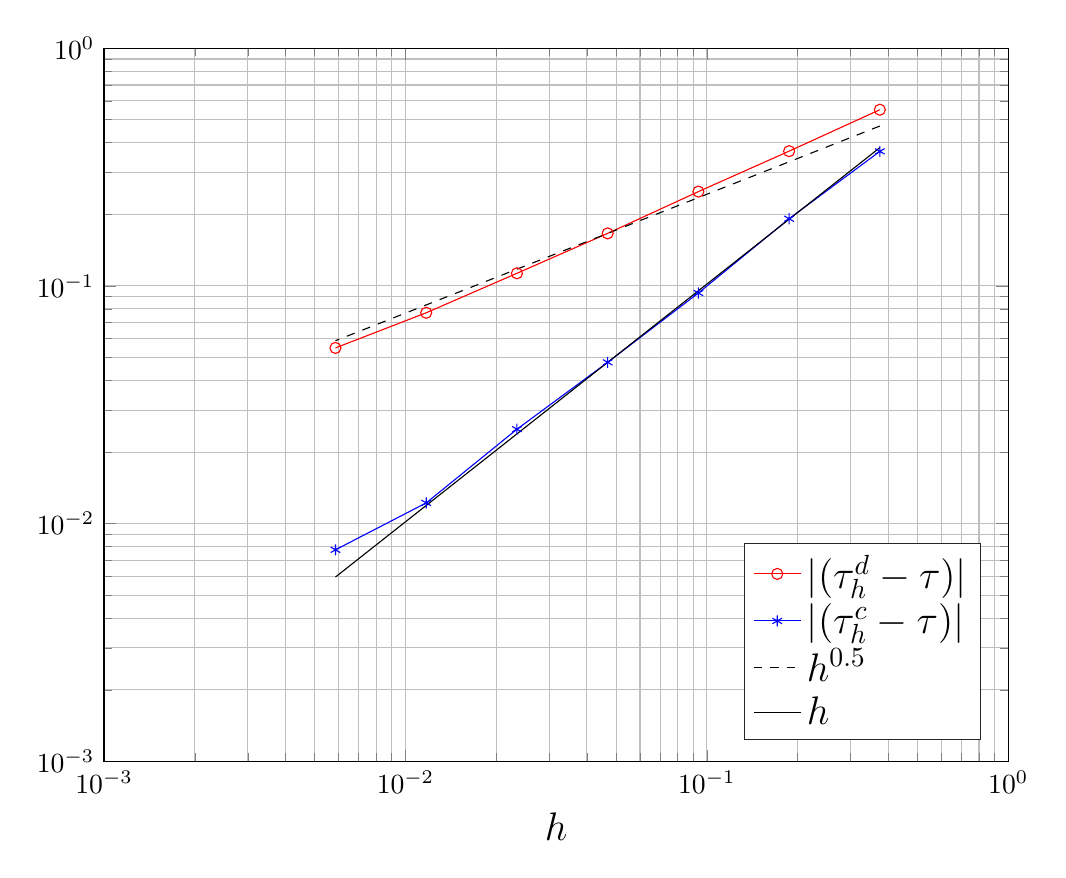
\begin{tikzpicture}

\begin{axis}[%
width=4.521in,
height=3.566in,
at={(0.758in,0.481in)},
scale only axis,
xmode=log,
xmin=0.001,
xmax=1,
xminorticks=true,
xlabel={$h$},
xlabel style={font=\Large},
xmajorgrids,
xminorgrids,
ymode=log,
ymin=0.001,
ymax=1,
yminorticks=true,
ymajorgrids,
yminorgrids,
axis background/.style={fill=white},
legend pos = south east,
legend style={legend cell align=left,align=left,draw=white!15!black,font=\Large}
]
\addplot [color=red,solid,mark=o,mark options={solid}]
  table[row sep=crcr]{%
0.375	0.550863107686105\\
0.1875	0.368781857686105\\
0.09375	0.249241232686105\\
0.046875	0.166314670186105\\
0.0234375	0.112973263936105\\
0.01171875	0.077078732686105\\
0.005859375	0.054845920186105\\
};
\addlegendentry{$|\E(\tau_h^d - \tau)|$};

\addplot [color=blue,solid,mark=asterisk,mark options={solid}]
  table[row sep=crcr]{%
0.375	0.368013107686105\\
0.1875	0.191688107686105\\
0.09375	0.0933443576861051\\
0.046875	0.047697482686105\\
0.0234375	0.024953732686105\\
0.01171875	0.012223654561105\\
0.005859375	0.00776291237360505\\
};
\addlegendentry{$|\E(\tau_h^c - \tau)|$};

\addplot [color=black,dashed]
  table[row sep=crcr]{%
0.375	0.470408924397596\\
0.1875	0.33262934037221\\
0.09375	0.235204462198798\\
0.046875	0.166314670186105\\
0.0234375	0.117602231099399\\
0.01171875	0.0831573350930525\\
0.005859375	0.0588011155496995\\
};
\addlegendentry{$h^{0.5}$};

\addplot [color=black,solid]
  table[row sep=crcr]{%
0.375	0.38157986148884\\
0.1875	0.19078993074442\\
0.09375	0.0953949653722099\\
0.046875	0.047697482686105\\
0.0234375	0.0238487413430525\\
0.01171875	0.0119243706715262\\
0.005859375	0.00596218533576312\\
};
\addlegendentry{$h$};

\end{axis}
\end{tikzpicture}%
 }  
        \caption{Convergence of CEM and DEM.}
        \label{fig:KillTwoD}
    \end{subfigure}
    \begin{subfigure}{0.49\linewidth}
        \centering
        \resizebox{1\linewidth}{!}{% This file was created by matlab2tikz.
%
%The latest updates can be retrieved from
%  http://www.mathworks.com/matlabcentral/fileexchange/22022-matlab2tikz-matlab2tikz
%where you can also make suggestions and rate matlab2tikz.
%
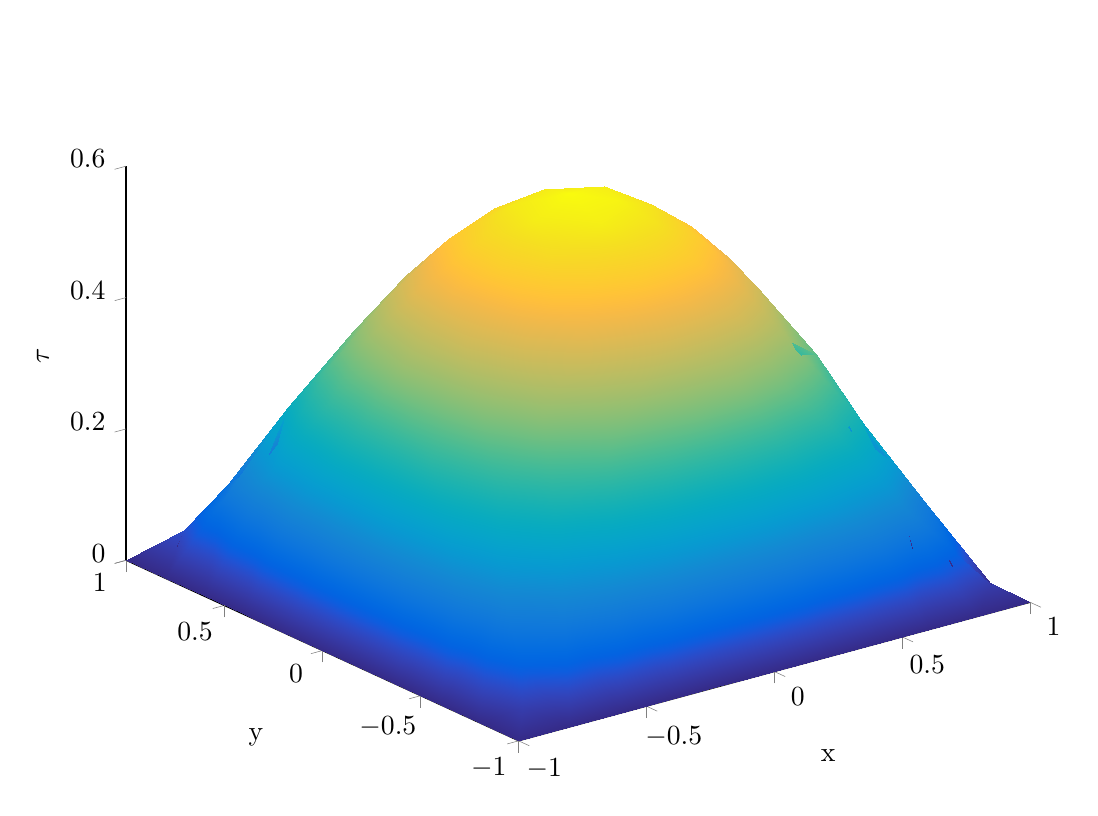
\begin{tikzpicture}

\begin{axis}[%
width=4.521in,
height=3.566in,
at={(0.758in,0.481in)},
scale only axis,
colormap={mymap}{[1pt] rgb(0pt)=(0.2081,0.1663,0.5292); rgb(1pt)=(0.211624,0.189781,0.577676); rgb(2pt)=(0.212252,0.213771,0.626971); rgb(3pt)=(0.2081,0.2386,0.677086); rgb(4pt)=(0.195905,0.264457,0.7279); rgb(5pt)=(0.170729,0.291938,0.779248); rgb(6pt)=(0.125271,0.324243,0.830271); rgb(7pt)=(0.0591333,0.359833,0.868333); rgb(8pt)=(0.0116952,0.38751,0.881957); rgb(9pt)=(0.00595714,0.408614,0.882843); rgb(10pt)=(0.0165143,0.4266,0.878633); rgb(11pt)=(0.0328524,0.443043,0.871957); rgb(12pt)=(0.0498143,0.458571,0.864057); rgb(13pt)=(0.0629333,0.47369,0.855438); rgb(14pt)=(0.0722667,0.488667,0.8467); rgb(15pt)=(0.0779429,0.503986,0.838371); rgb(16pt)=(0.0793476,0.520024,0.831181); rgb(17pt)=(0.0749429,0.537543,0.826271); rgb(18pt)=(0.0640571,0.556986,0.823957); rgb(19pt)=(0.0487714,0.577224,0.822829); rgb(20pt)=(0.0343429,0.596581,0.819852); rgb(21pt)=(0.0265,0.6137,0.8135); rgb(22pt)=(0.0238905,0.628662,0.803762); rgb(23pt)=(0.0230905,0.641786,0.791267); rgb(24pt)=(0.0227714,0.653486,0.776757); rgb(25pt)=(0.0266619,0.664195,0.760719); rgb(26pt)=(0.0383714,0.674271,0.743552); rgb(27pt)=(0.0589714,0.683757,0.725386); rgb(28pt)=(0.0843,0.692833,0.706167); rgb(29pt)=(0.113295,0.7015,0.685857); rgb(30pt)=(0.145271,0.709757,0.664629); rgb(31pt)=(0.180133,0.717657,0.642433); rgb(32pt)=(0.217829,0.725043,0.619262); rgb(33pt)=(0.258643,0.731714,0.595429); rgb(34pt)=(0.302171,0.737605,0.571186); rgb(35pt)=(0.348167,0.742433,0.547267); rgb(36pt)=(0.395257,0.7459,0.524443); rgb(37pt)=(0.44201,0.748081,0.503314); rgb(38pt)=(0.487124,0.749062,0.483976); rgb(39pt)=(0.530029,0.749114,0.466114); rgb(40pt)=(0.570857,0.748519,0.44939); rgb(41pt)=(0.609852,0.747314,0.433686); rgb(42pt)=(0.6473,0.7456,0.4188); rgb(43pt)=(0.683419,0.743476,0.404433); rgb(44pt)=(0.71841,0.741133,0.390476); rgb(45pt)=(0.752486,0.7384,0.376814); rgb(46pt)=(0.785843,0.735567,0.363271); rgb(47pt)=(0.818505,0.732733,0.34979); rgb(48pt)=(0.850657,0.7299,0.336029); rgb(49pt)=(0.882433,0.727433,0.3217); rgb(50pt)=(0.913933,0.725786,0.306276); rgb(51pt)=(0.944957,0.726114,0.288643); rgb(52pt)=(0.973895,0.731395,0.266648); rgb(53pt)=(0.993771,0.745457,0.240348); rgb(54pt)=(0.999043,0.765314,0.216414); rgb(55pt)=(0.995533,0.786057,0.196652); rgb(56pt)=(0.988,0.8066,0.179367); rgb(57pt)=(0.978857,0.827143,0.163314); rgb(58pt)=(0.9697,0.848138,0.147452); rgb(59pt)=(0.962586,0.870514,0.1309); rgb(60pt)=(0.958871,0.8949,0.113243); rgb(61pt)=(0.959824,0.921833,0.0948381); rgb(62pt)=(0.9661,0.951443,0.0755333); rgb(63pt)=(0.9763,0.9831,0.0538)},
xmin=-1,
xmax=1,
tick align=outside,
xlabel={x},
ymin=-1,
ymax=1,
ylabel={y},
zmin=0,
zmax=0.6,
zlabel={$\tau$},
view={-37.5}{30},
axis background/.style={fill=white},
axis x line*=bottom,
axis y line*=left,
axis z line*=left
]

\addplot3[area legend,solid,table/row sep=crcr,patch,shader=interp,forget plot,patch table={%
0	1	2\\
3	4	5\\
6	7	8\\
9	10	11\\
12	13	14\\
15	16	17\\
18	19	20\\
21	22	23\\
24	25	26\\
27	28	29\\
30	31	32\\
33	34	35\\
36	37	38\\
39	40	41\\
42	43	44\\
45	46	47\\
48	49	50\\
51	52	53\\
54	55	56\\
57	58	59\\
60	61	62\\
63	64	65\\
66	67	68\\
69	70	71\\
72	73	74\\
75	76	77\\
78	79	80\\
81	82	83\\
84	85	86\\
87	88	89\\
90	91	92\\
93	94	95\\
96	97	98\\
99	100	101\\
102	103	104\\
105	106	107\\
108	109	110\\
111	112	113\\
114	115	116\\
117	118	119\\
120	121	122\\
123	124	125\\
126	127	128\\
129	130	131\\
132	133	134\\
135	136	137\\
138	139	140\\
141	142	143\\
144	145	146\\
147	148	149\\
150	151	152\\
153	154	155\\
156	157	158\\
159	160	161\\
162	163	164\\
165	166	167\\
168	169	170\\
171	172	173\\
174	175	176\\
177	178	179\\
180	181	182\\
183	184	185\\
186	187	188\\
189	190	191\\
192	193	194\\
195	196	197\\
198	199	200\\
201	202	203\\
204	205	206\\
207	208	209\\
210	211	212\\
213	214	215\\
216	217	218\\
219	220	221\\
222	223	224\\
225	226	227\\
228	229	230\\
231	232	233\\
234	235	236\\
237	238	239\\
240	241	242\\
243	244	245\\
246	247	248\\
249	250	251\\
252	253	254\\
255	256	257\\
258	259	260\\
261	262	263\\
264	265	266\\
267	268	269\\
270	271	272\\
273	274	275\\
276	277	278\\
279	280	281\\
282	283	284\\
285	286	287\\
288	289	290\\
291	292	293\\
294	295	296\\
297	298	299\\
300	301	302\\
303	304	305\\
306	307	308\\
309	310	311\\
312	313	314\\
315	316	317\\
318	319	320\\
321	322	323\\
324	325	326\\
327	328	329\\
330	331	332\\
333	334	335\\
336	337	338\\
339	340	341\\
342	343	344\\
345	346	347\\
348	349	350\\
351	352	353\\
354	355	356\\
357	358	359\\
360	361	362\\
363	364	365\\
366	367	368\\
369	370	371\\
372	373	374\\
375	376	377\\
378	379	380\\
381	382	383\\
384	385	386\\
387	388	389\\
390	391	392\\
393	394	395\\
396	397	398\\
399	400	401\\
402	403	404\\
405	406	407\\
408	409	410\\
411	412	413\\
414	415	416\\
417	418	419\\
420	421	422\\
423	424	425\\
426	427	428\\
429	430	431\\
432	433	434\\
435	436	437\\
438	439	440\\
441	442	443\\
444	445	446\\
447	448	449\\
450	451	452\\
453	454	455\\
456	457	458\\
459	460	461\\
462	463	464\\
465	466	467\\
468	469	470\\
471	472	473\\
474	475	476\\
477	478	479\\
480	481	482\\
483	484	485\\
486	487	488\\
489	490	491\\
492	493	494\\
495	496	497\\
498	499	500\\
501	502	503\\
504	505	506\\
507	508	509\\
510	511	512\\
513	514	515\\
516	517	518\\
519	520	521\\
522	523	524\\
525	526	527\\
528	529	530\\
531	532	533\\
534	535	536\\
537	538	539\\
540	541	542\\
543	544	545\\
546	547	548\\
549	550	551\\
552	553	554\\
555	556	557\\
558	559	560\\
561	562	563\\
564	565	566\\
567	568	569\\
570	571	572\\
573	574	575\\
576	577	578\\
579	580	581\\
582	583	584\\
585	586	587\\
588	589	590\\
591	592	593\\
594	595	596\\
597	598	599\\
600	601	602\\
603	604	605\\
606	607	608\\
609	610	611\\
612	613	614\\
615	616	617\\
618	619	620\\
621	622	623\\
624	625	626\\
627	628	629\\
630	631	632\\
633	634	635\\
636	637	638\\
639	640	641\\
642	643	644\\
645	646	647\\
648	649	650\\
651	652	653\\
654	655	656\\
657	658	659\\
660	661	662\\
663	664	665\\
666	667	668\\
669	670	671\\
672	673	674\\
675	676	677\\
678	679	680\\
681	682	683\\
684	685	686\\
687	688	689\\
690	691	692\\
693	694	695\\
696	697	698\\
699	700	701\\
702	703	704\\
705	706	707\\
708	709	710\\
711	712	713\\
714	715	716\\
717	718	719\\
720	721	722\\
723	724	725\\
726	727	728\\
729	730	731\\
732	733	734\\
735	736	737\\
738	739	740\\
741	742	743\\
744	745	746\\
747	748	749\\
750	751	752\\
753	754	755\\
756	757	758\\
759	760	761\\
762	763	764\\
765	766	767\\
768	769	770\\
771	772	773\\
774	775	776\\
777	778	779\\
780	781	782\\
783	784	785\\
786	787	788\\
789	790	791\\
792	793	794\\
795	796	797\\
798	799	800\\
801	802	803\\
804	805	806\\
807	808	809\\
810	811	812\\
813	814	815\\
816	817	818\\
819	820	821\\
822	823	824\\
825	826	827\\
828	829	830\\
831	832	833\\
834	835	836\\
837	838	839\\
840	841	842\\
843	844	845\\
846	847	848\\
849	850	851\\
852	853	854\\
855	856	857\\
858	859	860\\
861	862	863\\
864	865	866\\
867	868	869\\
870	871	872\\
873	874	875\\
876	877	878\\
879	880	881\\
882	883	884\\
885	886	887\\
888	889	890\\
891	892	893\\
894	895	896\\
897	898	899\\
900	901	902\\
903	904	905\\
906	907	908\\
909	910	911\\
912	913	914\\
915	916	917\\
918	919	920\\
921	922	923\\
924	925	926\\
927	928	929\\
930	931	932\\
933	934	935\\
}]
table[row sep=crcr, point meta=\thisrow{c}] {%
x	y	z	c\\
-0.8	1	0	0\\
-1	1	0	0\\
-0.870979864217162	0.874090623781756	0.0503358598117232	0.0503358598117232\\
-0.6	1	0	0\\
-0.8	1	0	0\\
-0.715759069893515	0.851783447512538	0.1063700540631	0.1063700540631\\
-0.4	1	0	0\\
-0.6	1	0	0\\
-0.553557227232278	0.85599352174284	0.134555464783061	0.134555464783061\\
-0.2	1	0	0\\
-0.4	1	0	0\\
-0.256371139537587	0.844436132195903	0.177771244732144	0.177771244732144\\
0	1	0	0\\
-0.2	1	0	0\\
-0.123171927132804	0.882407229449651	0.141599115239887	0.141599115239887\\
0.2	1	0	0\\
0	1	0	0\\
0.138576080047019	0.836444863570092	0.192526814683977	0.192526814683977\\
0.4	1	0	0\\
0.2	1	0	0\\
0.314746867281053	0.841650113118016	0.176869739222543	0.176869739222543\\
0.6	1	0	0\\
0.4	1	0	0\\
0.500557557249754	0.834821560479383	0.161211039480775	0.161211039480775\\
1	0.8	0	0\\
1	1	0	0\\
0.913245437763783	0.903908655259532	0.029200764250968	0.029200764250968\\
0.8	1	0	0\\
0.6	1	0	0\\
0.6908636124721	0.827426566529025	0.127146907841705	0.127146907841705\\
1	1	0	0\\
0.8	1	0	0\\
0.913245437763783	0.903908655259532	0.029200764250968	0.029200764250968\\
0.913245437763783	0.903908655259532	0.029200764250968	0.029200764250968\\
0.8	1	0	0\\
0.853111865010539	0.81689479082676	0.0774114970720003	0.0774114970720003\\
1	0.6	0	0\\
1	0.8	0	0\\
0.913257156072776	0.71766207885242	0.0641486951792736	0.0641486951792736\\
1	0.4	0	0\\
1	0.6	0	0\\
0.858172452446661	0.489687445107711	0.140968616362916	0.140968616362916\\
1	0.2	0	0\\
1	0.4	0	0\\
0.801876020058965	0.306586241275605	0.217067338383388	0.217067338383388\\
1	-0.2	0	0\\
1	0	0	0\\
0.842830738889788	-0.109162193087545	0.186555603301951	0.186555603301951\\
1	-0.4	0	0\\
1	-0.2	0	0\\
0.839553137409186	-0.294644298019888	0.180743581899484	0.180743581899484\\
1	-0.6	0	0\\
1	-0.4	0	0\\
0.825961266928206	-0.490102064147121	0.170054775004226	0.170054775004226\\
0.8	-1	0	0\\
1	-1	0	0\\
0.903543131650638	-0.913183857559471	0.0292439041425551	0.0292439041425551\\
1	-0.8	0	0\\
1	-0.6	0	0\\
0.822757598423982	-0.688930059869196	0.130359222949275	0.130359222949275\\
1	-1	0	0\\
1	-0.8	0	0\\
0.903543131650638	-0.913183857559471	0.0292439041425551	0.0292439041425551\\
0.903543131650638	-0.913183857559471	0.0292439041425551	0.0292439041425551\\
1	-0.8	0	0\\
0.815246907920555	-0.852962033044177	0.07802448667025	0.07802448667025\\
0.6	-1	0	0\\
0.8	-1	0	0\\
0.716262971529556	-0.913440138799354	0.0643591564167846	0.0643591564167846\\
0.4	-1	0	0\\
0.6	-1	0	0\\
0.486610676987292	-0.860815662729556	0.139125923998322	0.139125923998322\\
0.2	-1	0	0\\
0.4	-1	0	0\\
0.30415666992098	-0.806486553345674	0.212859546091864	0.212859546091864\\
-0.2	-1	0	0\\
0	-1	0	0\\
-0.108836774839956	-0.842631178463089	0.186853940747798	0.186853940747798\\
-0.4	-1	0	0\\
-0.2	-1	0	0\\
-0.295155054484333	-0.839202734226978	0.181080208857889	0.181080208857889\\
-0.6	-1	0	0\\
-0.4	-1	0	0\\
-0.491181950150036	-0.827450133500077	0.168514322976903	0.168514322976903\\
-1	-0.8	0	0\\
-1	-1	0	0\\
-0.913179600822541	-0.903978796898105	0.0292292069096813	0.0292292069096813\\
-0.8	-1	0	0\\
-0.6	-1	0	0\\
-0.689383148912005	-0.825669061227738	0.128443225229467	0.128443225229467\\
-1	-1	0	0\\
-0.8	-1	0	0\\
-0.913179600822541	-0.903978796898105	0.0292292069096813	0.0292292069096813\\
-0.913179600822541	-0.903978796898105	0.0292292069096813	0.0292292069096813\\
-0.8	-1	0	0\\
-0.852930471573381	-0.817084814175369	0.0774874322644484	0.0774874322644484\\
-1	-0.6	0	0\\
-1	-0.8	0	0\\
-0.913349182557632	-0.71824277938499	0.0639981239363015	0.0639981239363015\\
-1	-0.4	0	0\\
-1	-0.6	0	0\\
-0.858612569930114	-0.502582179815703	0.138892582617845	0.138892582617845\\
-1	-0.2	0	0\\
-1	-0.4	0	0\\
-0.875147249859378	-0.2495178793164	0.145482917588398	0.145482917588398\\
0.822757598423982	-0.688930059869196	0.130359222949275	0.130359222949275\\
1	-0.6	0	0\\
0.825961266928206	-0.490102064147121	0.170054775004226	0.170054775004226\\
-1	0.2	0	0\\
-1	0	0	0\\
-0.878430687062504	0.0687937548368703	0.147100833393107	0.147100833393107\\
-1	0.4	0	0\\
-1	0.2	0	0\\
-0.858638192546528	0.336283758462884	0.156024411502294	0.156024411502294\\
0.314746867281053	0.841650113118016	0.176869739222543	0.176869739222543\\
0.2	1	0	0\\
0.138576080047019	0.836444863570092	0.192526814683977	0.192526814683977\\
-1	0.6	0	0\\
-1	0.4	0	0\\
-0.81542002432126	0.514265339146589	0.176422646100678	0.176422646100678\\
-1	0	0	0\\
-1	-0.2	0	0\\
-0.849550627410001	-0.0857161204413969	0.181287438145949	0.181287438145949\\
-0.81542002432126	0.514265339146589	0.176422646100678	0.176422646100678\\
-1	0.4	0	0\\
-0.858638192546528	0.336283758462884	0.156024411502294	0.156024411502294\\
0	-1	0	0\\
0.2	-1	0	0\\
0.0842448278397462	-0.826656651009239	0.204706996767319	0.204706996767319\\
-0.295155054484333	-0.839202734226978	0.181080208857889	0.181080208857889\\
-0.2	-1	0	0\\
-0.108836774839956	-0.842631178463089	0.186853940747798	0.186853940747798\\
1	0	0	0\\
1	0.2	0	0\\
0.825000730866433	0.0840636812185947	0.20640087112894	0.20640087112894\\
0.839553137409186	-0.294644298019888	0.180743581899484	0.180743581899484\\
1	-0.2	0	0\\
0.842830738889788	-0.109162193087545	0.186555603301951	0.186555603301951\\
-0.421476522111469	0.76529746608585	0.231757594594101	0.231757594594101\\
-0.4	1	0	0\\
-0.553557227232278	0.85599352174284	0.134555464783061	0.134555464783061\\
-1	1	0	0\\
-1	0.8	0	0\\
-0.870979864217162	0.874090623781756	0.0503358598117232	0.0503358598117232\\
-1	0.8	0	0\\
-1	0.6	0	0\\
-0.838909094432717	0.717165597536304	0.113672221435356	0.113672221435356\\
-0.870979864217162	0.874090623781756	0.0503358598117232	0.0503358598117232\\
-1	0.8	0	0\\
-0.838909094432717	0.717165597536304	0.113672221435356	0.113672221435356\\
-0.689383148912005	-0.825669061227738	0.128443225229467	0.128443225229467\\
-0.6	-1	0	0\\
-0.491181950150036	-0.827450133500077	0.168514322976903	0.168514322976903\\
0.162899107774523	0.0782930267751429	0.573283948704444	0.573283948704444\\
-0.0145232187187818	0.0259493451768655	0.588597916020823	0.588597916020823\\
0.0995954131227801	-0.0711056079718885	0.580192879465293	0.580192879465293\\
0.6908636124721	0.827426566529025	0.127146907841705	0.127146907841705\\
0.6	1	0	0\\
0.500557557249754	0.834821560479383	0.161211039480775	0.161211039480775\\
-0.0437189086592884	-0.1794562797288	0.573870426458542	0.573870426458542\\
-0.0145232187187818	0.0259493451768655	0.588597916020823	0.588597916020823\\
-0.183666461200581	-0.0196981175980336	0.572015059946271	0.572015059946271\\
-0.183666461200581	-0.0196981175980336	0.572015059946271	0.572015059946271\\
-0.0145232187187818	0.0259493451768655	0.588597916020823	0.588597916020823\\
-0.143244730260345	0.15312684048721	0.567139291819697	0.567139291819697\\
-0.573742666641828	0.478792000601255	0.335991863885408	0.335991863885408\\
-0.435775856529045	0.402580883145608	0.423498389275608	0.423498389275608\\
-0.436448993108287	0.574739898722634	0.349979922598284	0.349979922598284\\
-0.777645420963466	0.191713474052978	0.24812819524673	0.24812819524673\\
-1	0.2	0	0\\
-0.878430687062504	0.0687937548368703	0.147100833393107	0.147100833393107\\
-0.308985524220196	-0.434191396690207	0.453727811443478	0.453727811443478\\
-0.44256229481138	-0.30475784338953	0.450675141546866	0.450675141546866\\
-0.504626867096141	-0.476494146294975	0.370506581998038	0.370506581998038\\
0.30415666992098	-0.806486553345674	0.212859546091864	0.212859546091864\\
0.4	-1	0	0\\
0.486610676987292	-0.860815662729556	0.139125923998322	0.139125923998322\\
0.0893690793198263	-0.463478876426208	0.474487006103424	0.474487006103424\\
0.261928641455601	-0.488055957894452	0.438978374350292	0.438978374350292\\
0.2060410026947	-0.342035240885369	0.510200300431043	0.510200300431043\\
0.801876020058965	0.306586241275605	0.217067338383388	0.217067338383388\\
1	0.4	0	0\\
0.858172452446661	0.489687445107711	0.140968616362916	0.140968616362916\\
0.500557557249754	0.834821560479383	0.161211039480775	0.161211039480775\\
0.4	1	0	0\\
0.314746867281053	0.841650113118016	0.176869739222543	0.176869739222543\\
-0.0174658545926647	0.801898927302032	0.229884764941956	0.229884764941956\\
0	1	0	0\\
-0.123171927132804	0.882407229449651	0.141599115239887	0.141599115239887\\
0.629591208237007	0.150059132096618	0.371703125936085	0.371703125936085\\
0.464005364535939	0.260203010616371	0.451392983448571	0.451392983448571\\
0.457941066948159	0.074681360252563	0.478108938985459	0.478108938985459\\
-0.536183382478912	-0.125067364855863	0.434419852807405	0.434419852807405\\
-0.44256229481138	-0.30475784338953	0.450675141546866	0.450675141546866\\
-0.376489904228021	-0.187383275146088	0.499799124231866	0.499799124231866\\
0.825961266928206	-0.490102064147121	0.170054775004226	0.170054775004226\\
1	-0.4	0	0\\
0.839553137409186	-0.294644298019888	0.180743581899484	0.180743581899484\\
-0.491181950150036	-0.827450133500077	0.168514322976903	0.168514322976903\\
-0.4	-1	0	0\\
-0.295155054484333	-0.839202734226978	0.181080208857889	0.181080208857889\\
0.151932036409303	-0.636460365815934	0.366462112770309	0.366462112770309\\
0.261928641455601	-0.488055957894452	0.438978374350292	0.438978374350292\\
0.0893690793198263	-0.463478876426208	0.474487006103424	0.474487006103424\\
-0.31111533158028	-0.281732042536466	0.501981892837586	0.501981892837586\\
-0.241660277500026	-0.172513969577467	0.544861710314016	0.544861710314016\\
-0.376489904228021	-0.187383275146088	0.499799124231866	0.499799124231866\\
-0.796122724389227	-0.361886425045465	0.214012852098144	0.214012852098144\\
-0.695084883753552	-0.495926997595022	0.263405412558248	0.263405412558248\\
-0.617615903555302	-0.32670910304294	0.35341227577042	0.35341227577042\\
0.321736948673632	-0.218404805181936	0.515022791117278	0.515022791117278\\
0.149400916774043	-0.200302697508326	0.557599295554639	0.557599295554639\\
0.2060410026947	-0.342035240885369	0.510200300431043	0.510200300431043\\
0.459725917575231	0.478817132146761	0.389012381461728	0.389012381461728\\
0.464005364535939	0.260203010616371	0.451392983448571	0.451392983448571\\
0.609248416595618	0.336700564235885	0.355920940303567	0.355920940303567\\
-0.591992818593216	-0.654470500305776	0.255730623027946	0.255730623027946\\
-0.368952164395011	-0.646051178924541	0.32789689044595	0.32789689044595\\
-0.504626867096141	-0.476494146294975	0.370506581998038	0.370506581998038\\
0.646526572158138	-0.5892372548303	0.261059443004205	0.261059443004205\\
0.647783933105589	-0.365727428795828	0.32753780854032	0.32753780854032\\
0.453484147433517	-0.490455219207141	0.386061114641414	0.386061114641414\\
-0.8	1	0	0\\
-0.870979864217162	0.874090623781756	0.0503358598117232	0.0503358598117232\\
-0.715759069893515	0.851783447512538	0.1063700540631	0.1063700540631\\
-0.436448993108287	0.574739898722634	0.349979922598284	0.349979922598284\\
-0.435775856529045	0.402580883145608	0.423498389275608	0.423498389275608\\
-0.305196827885855	0.481941510996423	0.431183963802012	0.431183963802012\\
0.651531723544283	-0.800304145152872	0.15673981059701	0.15673981059701\\
0.6	-1	0	0\\
0.716262971529556	-0.913440138799354	0.0643591564167846	0.0643591564167846\\
0.651531723544283	-0.800304145152872	0.15673981059701	0.15673981059701\\
0.822757598423982	-0.688930059869196	0.130359222949275	0.130359222949275\\
0.646526572158138	-0.5892372548303	0.261059443004205	0.261059443004205\\
0.457941066948159	0.074681360252563	0.478108938985459	0.478108938985459\\
0.464005364535939	0.260203010616371	0.451392983448571	0.451392983448571\\
0.313359205867812	0.176240487473655	0.524936034219624	0.524936034219624\\
0.799426193403826	0.656174087711846	0.156000232172647	0.156000232172647\\
1	0.6	0	0\\
0.913257156072776	0.71766207885242	0.0641486951792736	0.0641486951792736\\
-0.800381152695487	-0.658205081403852	0.154847335186494	0.154847335186494\\
-1	-0.6	0	0\\
-0.913349182557632	-0.71824277938499	0.0639981239363015	0.0639981239363015\\
-0.800381152695487	-0.658205081403852	0.154847335186494	0.154847335186494\\
-0.689383148912005	-0.825669061227738	0.128443225229467	0.128443225229467\\
-0.591992818593216	-0.654470500305776	0.255730623027946	0.255730623027946\\
-0.131538906378604	0.468005506270669	0.469924617305817	0.469924617305817\\
0.0468419620052357	0.523978954343319	0.443742708621581	0.443742708621581\\
-0.0677763280124889	0.648507972991784	0.361033435408362	0.361033435408362\\
0.172508063347201	0.422930104621211	0.484063997084143	0.484063997084143\\
0.0468419620052357	0.523978954343319	0.443742708621581	0.443742708621581\\
0.0285171270359044	0.362157622648837	0.521278659914479	0.521278659914479\\
0.453484147433517	-0.490455219207141	0.386061114641414	0.386061114641414\\
0.261928641455601	-0.488055957894452	0.438978374350292	0.438978374350292\\
0.32991065048365	-0.623943472007708	0.347897178937779	0.347897178937779\\
0.0893690793198263	-0.463478876426208	0.474487006103424	0.474487006103424\\
-0.0468923144628943	-0.37201189317892	0.516612875922252	0.516612875922252\\
-0.0519572972000214	-0.516668038614571	0.447206394227684	0.447206394227684\\
0.801876020058965	0.306586241275605	0.217067338383388	0.217067338383388\\
0.687082418720278	0.487393175878324	0.271787481430287	0.271787481430287\\
0.609248416595618	0.336700564235885	0.355920940303567	0.355920940303567\\
0.457941066948159	0.074681360252563	0.478108938985459	0.478108938985459\\
0.386220146013541	-0.0691483215457924	0.509515390249842	0.509515390249842\\
0.521855887175084	-0.0613271652026621	0.443724996577735	0.443724996577735\\
0.0893728715906334	0.678554065055819	0.337074523808599	0.337074523808599\\
0.0468419620052357	0.523978954343319	0.443742708621581	0.443742708621581\\
0.193142943255321	0.563632036809665	0.407797185144958	0.407797185144958\\
-0.467792458521678	0.219937427890346	0.457907133070784	0.457907133070784\\
-0.435775856529045	0.402580883145608	0.423498389275608	0.423498389275608\\
-0.560240270361451	0.344844062180542	0.380926635012534	0.380926635012534\\
0.0172621493060368	0.196448852647962	0.569192003743179	0.569192003743179\\
0.167453556422288	0.263155683226473	0.540735468359687	0.540735468359687\\
0.0285171270359044	0.362157622648837	0.521278659914479	0.521278659914479\\
-0.777645420963466	0.191713474052978	0.24812819524673	0.24812819524673\\
-0.617913717697813	0.079971000861777	0.383870428360901	0.383870428360901\\
-0.624616411644707	0.242665578371416	0.361275369549205	0.361275369549205\\
-0.536183382478912	-0.125067364855863	0.434419852807405	0.434419852807405\\
-0.617913717697813	0.079971000861777	0.383870428360901	0.383870428360901\\
-0.699519166874299	-0.0584145433376073	0.320912054383973	0.320912054383973\\
-0.421476522111469	0.76529746608585	0.231757594594101	0.231757594594101\\
-0.629666025324687	0.659481894250005	0.24105814130584	0.24105814130584\\
-0.436448993108287	0.574739898722634	0.349979922598284	0.349979922598284\\
-0.467792458521678	0.219937427890346	0.457907133070784	0.457907133070784\\
-0.617913717697813	0.079971000861777	0.383870428360901	0.383870428360901\\
-0.456541297467842	0.0462574378515442	0.478943897003244	0.478943897003244\\
-0.796122724389227	-0.361886425045465	0.214012852098144	0.214012852098144\\
-1	-0.4	0	0\\
-0.858612569930114	-0.502582179815703	0.138892582617845	0.138892582617845\\
0.30415666992098	-0.806486553345674	0.212859546091864	0.212859546091864\\
0.478214140797659	-0.695585476223675	0.268723097640064	0.268723097640064\\
0.32991065048365	-0.623943472007708	0.347897178937779	0.347897178937779\\
-0.350427977113875	-0.0568798710953585	0.524639252238995	0.524639252238995\\
-0.241660277500026	-0.172513969577467	0.544861710314016	0.544861710314016\\
-0.183666461200581	-0.0196981175980336	0.572015059946271	0.572015059946271\\
0.521855887175084	-0.0613271652026621	0.443724996577735	0.443724996577735\\
0.386220146013541	-0.0691483215457924	0.509515390249842	0.509515390249842\\
0.456651668322266	-0.168447833276863	0.467989266720155	0.467989266720155\\
-0.256371139537587	0.844436132195903	0.177771244732144	0.177771244732144\\
-0.251840934393812	0.65073582839654	0.34432188663096	0.34432188663096\\
-0.14310781983293	0.765817634248709	0.258702609329505	0.258702609329505\\
1	0.8	0	0\\
0.913245437763783	0.903908655259532	0.029200764250968	0.029200764250968\\
0.853111865010539	0.81689479082676	0.0774114970720003	0.0774114970720003\\
-0.131538906378604	0.468005506270669	0.469924617305817	0.469924617305817\\
-0.0999792356165469	0.29750658388758	0.53828138268099	0.53828138268099\\
0.0285171270359044	0.362157622648837	0.521278659914479	0.521278659914479\\
0.799426193403826	0.656174087711846	0.156000232172647	0.156000232172647\\
0.687082418720278	0.487393175878324	0.271787481430287	0.271787481430287\\
0.858172452446661	0.489687445107711	0.140968616362916	0.140968616362916\\
0.239679041234336	-0.0747988778282174	0.556617424129489	0.556617424129489\\
0.386220146013541	-0.0691483215457924	0.509515390249842	0.509515390249842\\
0.312829618686655	0.0361464359017708	0.537102152866081	0.537102152866081\\
0.651531723544283	-0.800304145152872	0.15673981059701	0.15673981059701\\
0.478214140797659	-0.695585476223675	0.268723097640064	0.268723097640064\\
0.486610676987292	-0.860815662729556	0.139125923998322	0.139125923998322\\
-0.0437189086592884	-0.1794562797288	0.573870426458542	0.573870426458542\\
-0.0468923144628943	-0.37201189317892	0.516612875922252	0.516612875922252\\
0.0706839927525276	-0.312287735493971	0.535778389231988	0.535778389231988\\
-0.617615903555302	-0.32670910304294	0.35341227577042	0.35341227577042\\
-0.695084883753552	-0.495926997595022	0.263405412558248	0.263405412558248\\
-0.504626867096141	-0.476494146294975	0.370506581998038	0.370506581998038\\
-0.308985524220196	-0.434191396690207	0.453727811443478	0.453727811443478\\
-0.368952164395011	-0.646051178924541	0.32789689044595	0.32789689044595\\
-0.188699779816531	-0.572089273359516	0.403567007447756	0.403567007447756\\
0.467892646677106	-0.300972929247376	0.439346124229837	0.439346124229837\\
0.647783933105589	-0.365727428795828	0.32753780854032	0.32753780854032\\
0.581538749766835	-0.190353470678335	0.397087747832545	0.397087747832545\\
0.321736948673632	-0.218404805181936	0.515022791117278	0.515022791117278\\
0.386220146013541	-0.0691483215457924	0.509515390249842	0.509515390249842\\
0.239679041234336	-0.0747988778282174	0.556617424129489	0.556617424129489\\
0.6908636124721	0.827426566529025	0.127146907841705	0.127146907841705\\
0.500557557249754	0.834821560479383	0.161211039480775	0.161211039480775\\
0.590963022235164	0.660549521945042	0.253161809954322	0.253161809954322\\
0.590963022235164	0.660549521945042	0.253161809954322	0.253161809954322\\
0.500557557249754	0.834821560479383	0.161211039480775	0.161211039480775\\
0.404778435204039	0.681910640519122	0.295230923900934	0.295230923900934\\
-0.838909094432717	0.717165597536304	0.113672221435356	0.113672221435356\\
-1	0.6	0	0\\
-0.81542002432126	0.514265339146589	0.176422646100678	0.176422646100678\\
-0.573742666641828	0.478792000601255	0.335991863885408	0.335991863885408\\
-0.629666025324687	0.659481894250005	0.24105814130584	0.24105814130584\\
-0.67998691843914	0.507882653342416	0.265777528317003	0.265777528317003\\
-1	-0.8	0	0\\
-0.913179600822541	-0.903978796898105	0.0292292069096813	0.0292292069096813\\
-0.852930471573381	-0.817084814175369	0.0774874322644484	0.0774874322644484\\
-0.491181950150036	-0.827450133500077	0.168514322976903	0.168514322976903\\
-0.368952164395011	-0.646051178924541	0.32789689044595	0.32789689044595\\
-0.591992818593216	-0.654470500305776	0.255730623027946	0.255730623027946\\
0.590963022235164	0.660549521945042	0.253161809954322	0.253161809954322\\
0.687082418720278	0.487393175878324	0.271787481430287	0.271787481430287\\
0.799426193403826	0.656174087711846	0.156000232172647	0.156000232172647\\
0.6908636124721	0.827426566529025	0.127146907841705	0.127146907841705\\
0.590963022235164	0.660549521945042	0.253161809954322	0.253161809954322\\
0.799426193403826	0.656174087711846	0.156000232172647	0.156000232172647\\
0.8	-1	0	0\\
0.903543131650638	-0.913183857559471	0.0292439041425551	0.0292439041425551\\
0.815246907920555	-0.852962033044177	0.07802448667025	0.07802448667025\\
0.825961266928206	-0.490102064147121	0.170054775004226	0.170054775004226\\
0.647783933105589	-0.365727428795828	0.32753780854032	0.32753780854032\\
0.646526572158138	-0.5892372548303	0.261059443004205	0.261059443004205\\
-0.188699779816531	-0.572089273359516	0.403567007447756	0.403567007447756\\
-0.368952164395011	-0.646051178924541	0.32789689044595	0.32789689044595\\
-0.201012514379659	-0.715085349646872	0.298990929979058	0.298990929979058\\
-0.536183382478912	-0.125067364855863	0.434419852807405	0.434419852807405\\
-0.729105054552535	-0.200822554621074	0.289316387960488	0.289316387960488\\
-0.617615903555302	-0.32670910304294	0.35341227577042	0.35341227577042\\
0.581538749766835	-0.190353470678335	0.397087747832545	0.397087747832545\\
0.647783933105589	-0.365727428795828	0.32753780854032	0.32753780854032\\
0.717419694116031	-0.201076983778939	0.29696928072587	0.29696928072587\\
0.151932036409303	-0.636460365815934	0.366462112770309	0.366462112770309\\
0.30415666992098	-0.806486553345674	0.212859546091864	0.212859546091864\\
0.32991065048365	-0.623943472007708	0.347897178937779	0.347897178937779\\
-0.0519572972000214	-0.516668038614571	0.447206394227684	0.447206394227684\\
-0.0468923144628943	-0.37201189317892	0.516612875922252	0.516612875922252\\
-0.156991111184629	-0.442497792882714	0.476170525903155	0.476170525903155\\
-0.31111533158028	-0.281732042536466	0.501981892837586	0.501981892837586\\
-0.308985524220196	-0.434191396690207	0.453727811443478	0.453727811443478\\
-0.185241010817594	-0.314270126024311	0.522560644927547	0.522560644927547\\
-0.467792458521678	0.219937427890346	0.457907133070784	0.457907133070784\\
-0.311591314295825	0.109324344546677	0.534314000243037	0.534314000243037\\
-0.270562051272334	0.305759011517556	0.509763309393006	0.509763309393006\\
0.162899107774523	0.0782930267751429	0.573283948704444	0.573283948704444\\
0.167453556422288	0.263155683226473	0.540735468359687	0.540735468359687\\
0.0172621493060368	0.196448852647962	0.569192003743179	0.569192003743179\\
0.629591208237007	0.150059132096618	0.371703125936085	0.371703125936085\\
0.801876020058965	0.306586241275605	0.217067338383388	0.217067338383388\\
0.609248416595618	0.336700564235885	0.355920940303567	0.355920940303567\\
0.314746867281053	0.841650113118016	0.176869739222543	0.176869739222543\\
0.243215438556557	0.696935801995676	0.309845401353432	0.309845401353432\\
0.404778435204039	0.681910640519122	0.295230923900934	0.295230923900934\\
-0.421476522111469	0.76529746608585	0.231757594594101	0.231757594594101\\
-0.251840934393812	0.65073582839654	0.34432188663096	0.34432188663096\\
-0.256371139537587	0.844436132195903	0.177771244732144	0.177771244732144\\
0.404778435204039	0.681910640519122	0.295230923900934	0.295230923900934\\
0.243215438556557	0.696935801995676	0.309845401353432	0.309845401353432\\
0.318221535321866	0.579996560046282	0.376283328983717	0.376283328983717\\
0.581538749766835	-0.190353470678335	0.397087747832545	0.397087747832545\\
0.671060117555799	-0.0425238644998574	0.345139590286008	0.345139590286008\\
0.521855887175084	-0.0613271652026621	0.443724996577735	0.443724996577735\\
0.842830738889788	-0.109162193087545	0.186555603301951	0.186555603301951\\
1	0	0	0\\
0.825000730866433	0.0840636812185947	0.20640087112894	0.20640087112894\\
-0.188699779816531	-0.572089273359516	0.403567007447756	0.403567007447756\\
-0.0400681817402094	-0.67007462624905	0.346146999424569	0.346146999424569\\
-0.0519572972000214	-0.516668038614571	0.447206394227684	0.447206394227684\\
-0.108836774839956	-0.842631178463089	0.186853940747798	0.186853940747798\\
0	-1	0	0\\
0.0842448278397462	-0.826656651009239	0.204706996767319	0.204706996767319\\
-0.838909094432717	0.717165597536304	0.113672221435356	0.113672221435356\\
-0.629666025324687	0.659481894250005	0.24105814130584	0.24105814130584\\
-0.715759069893515	0.851783447512538	0.1063700540631	0.1063700540631\\
-0.131538906378604	0.468005506270669	0.469924617305817	0.469924617305817\\
-0.251840934393812	0.65073582839654	0.34432188663096	0.34432188663096\\
-0.305196827885855	0.481941510996423	0.431183963802012	0.431183963802012\\
-0.573742666641828	0.478792000601255	0.335991863885408	0.335991863885408\\
-0.698784277302622	0.374550558446254	0.288286607491356	0.288286607491356\\
-0.560240270361451	0.344844062180542	0.380926635012534	0.380926635012534\\
-0.849550627410001	-0.0857161204413969	0.181287438145949	0.181287438145949\\
-1	-0.2	0	0\\
-0.875147249859378	-0.2495178793164	0.145482917588398	0.145482917588398\\
0.629591208237007	0.150059132096618	0.371703125936085	0.371703125936085\\
0.671060117555799	-0.0425238644998574	0.345139590286008	0.345139590286008\\
0.825000730866433	0.0840636812185947	0.20640087112894	0.20640087112894\\
0.647783933105589	-0.365727428795828	0.32753780854032	0.32753780854032\\
0.825961266928206	-0.490102064147121	0.170054775004226	0.170054775004226\\
0.839553137409186	-0.294644298019888	0.180743581899484	0.180743581899484\\
0.151932036409303	-0.636460365815934	0.366462112770309	0.366462112770309\\
-0.0400681817402094	-0.67007462624905	0.346146999424569	0.346146999424569\\
0.0842448278397462	-0.826656651009239	0.204706996767319	0.204706996767319\\
-0.368952164395011	-0.646051178924541	0.32789689044595	0.32789689044595\\
-0.491181950150036	-0.827450133500077	0.168514322976903	0.168514322976903\\
-0.295155054484333	-0.839202734226978	0.181080208857889	0.181080208857889\\
-0.849550627410001	-0.0857161204413969	0.181287438145949	0.181287438145949\\
-0.729105054552535	-0.200822554621074	0.289316387960488	0.289316387960488\\
-0.699519166874299	-0.0584145433376073	0.320912054383973	0.320912054383973\\
-0.270562051272334	0.305759011517556	0.509763309393006	0.509763309393006\\
-0.311591314295825	0.109324344546677	0.534314000243037	0.534314000243037\\
-0.143244730260345	0.15312684048721	0.567139291819697	0.567139291819697\\
-0.44256229481138	-0.30475784338953	0.450675141546866	0.450675141546866\\
-0.308985524220196	-0.434191396690207	0.453727811443478	0.453727811443478\\
-0.31111533158028	-0.281732042536466	0.501981892837586	0.501981892837586\\
-0.251840934393812	0.65073582839654	0.34432188663096	0.34432188663096\\
-0.421476522111469	0.76529746608585	0.231757594594101	0.231757594594101\\
-0.436448993108287	0.574739898722634	0.349979922598284	0.349979922598284\\
-0.0437189086592884	-0.1794562797288	0.573870426458542	0.573870426458542\\
0.149400916774043	-0.200302697508326	0.557599295554639	0.557599295554639\\
0.0995954131227801	-0.0711056079718885	0.580192879465293	0.580192879465293\\
0.459725917575231	0.478817132146761	0.389012381461728	0.389012381461728\\
0.29046632350991	0.478227595927983	0.436123571072721	0.436123571072721\\
0.311159739978053	0.346682633914339	0.484379488422073	0.484379488422073\\
-0.695084883753552	-0.495926997595022	0.263405412558248	0.263405412558248\\
-0.800381152695487	-0.658205081403852	0.154847335186494	0.154847335186494\\
-0.591992818593216	-0.654470500305776	0.255730623027946	0.255730623027946\\
-0.689383148912005	-0.825669061227738	0.128443225229467	0.128443225229467\\
-0.491181950150036	-0.827450133500077	0.168514322976903	0.168514322976903\\
-0.591992818593216	-0.654470500305776	0.255730623027946	0.255730623027946\\
0.478214140797659	-0.695585476223675	0.268723097640064	0.268723097640064\\
0.651531723544283	-0.800304145152872	0.15673981059701	0.15673981059701\\
0.646526572158138	-0.5892372548303	0.261059443004205	0.261059443004205\\
0.822757598423982	-0.688930059869196	0.130359222949275	0.130359222949275\\
0.825961266928206	-0.490102064147121	0.170054775004226	0.170054775004226\\
0.646526572158138	-0.5892372548303	0.261059443004205	0.261059443004205\\
-0.777645420963466	0.191713474052978	0.24812819524673	0.24812819524673\\
-0.698784277302622	0.374550558446254	0.288286607491356	0.288286607491356\\
-0.858638192546528	0.336283758462884	0.156024411502294	0.156024411502294\\
-0.629666025324687	0.659481894250005	0.24105814130584	0.24105814130584\\
-0.838909094432717	0.717165597536304	0.113672221435356	0.113672221435356\\
-0.81542002432126	0.514265339146589	0.176422646100678	0.176422646100678\\
-0.870979864217162	0.874090623781756	0.0503358598117232	0.0503358598117232\\
-0.838909094432717	0.717165597536304	0.113672221435356	0.113672221435356\\
-0.715759069893515	0.851783447512538	0.1063700540631	0.1063700540631\\
-0.715759069893515	0.851783447512538	0.1063700540631	0.1063700540631\\
-0.629666025324687	0.659481894250005	0.24105814130584	0.24105814130584\\
-0.553557227232278	0.85599352174284	0.134555464783061	0.134555464783061\\
-0.44256229481138	-0.30475784338953	0.450675141546866	0.450675141546866\\
-0.536183382478912	-0.125067364855863	0.434419852807405	0.434419852807405\\
-0.617615903555302	-0.32670910304294	0.35341227577042	0.35341227577042\\
-0.800381152695487	-0.658205081403852	0.154847335186494	0.154847335186494\\
-0.695084883753552	-0.495926997595022	0.263405412558248	0.263405412558248\\
-0.858612569930114	-0.502582179815703	0.138892582617845	0.138892582617845\\
-0.698784277302622	0.374550558446254	0.288286607491356	0.288286607491356\\
-0.777645420963466	0.191713474052978	0.24812819524673	0.24812819524673\\
-0.624616411644707	0.242665578371416	0.361275369549205	0.361275369549205\\
-0.81542002432126	0.514265339146589	0.176422646100678	0.176422646100678\\
-0.698784277302622	0.374550558446254	0.288286607491356	0.288286607491356\\
-0.67998691843914	0.507882653342416	0.265777528317003	0.265777528317003\\
-0.617913717697813	0.079971000861777	0.383870428360901	0.383870428360901\\
-0.777645420963466	0.191713474052978	0.24812819524673	0.24812819524673\\
-0.764656987373661	0.0391649423298058	0.263986440397266	0.263986440397266\\
-0.796122724389227	-0.361886425045465	0.214012852098144	0.214012852098144\\
-0.729105054552535	-0.200822554621074	0.289316387960488	0.289316387960488\\
-0.875147249859378	-0.2495178793164	0.145482917588398	0.145482917588398\\
0.321736948673632	-0.218404805181936	0.515022791117278	0.515022791117278\\
0.467892646677106	-0.300972929247376	0.439346124229837	0.439346124229837\\
0.456651668322266	-0.168447833276863	0.467989266720155	0.467989266720155\\
0.842830738889788	-0.109162193087545	0.186555603301951	0.186555603301951\\
0.671060117555799	-0.0425238644998574	0.345139590286008	0.345139590286008\\
0.717419694116031	-0.201076983778939	0.29696928072587	0.29696928072587\\
-0.185241010817594	-0.314270126024311	0.522560644927547	0.522560644927547\\
-0.308985524220196	-0.434191396690207	0.453727811443478	0.453727811443478\\
-0.156991111184629	-0.442497792882714	0.476170525903155	0.476170525903155\\
-0.108836774839956	-0.842631178463089	0.186853940747798	0.186853940747798\\
-0.0400681817402094	-0.67007462624905	0.346146999424569	0.346146999424569\\
-0.201012514379659	-0.715085349646872	0.298990929979058	0.298990929979058\\
0.2	-1	0	0\\
0.30415666992098	-0.806486553345674	0.212859546091864	0.212859546091864\\
0.0842448278397462	-0.826656651009239	0.204706996767319	0.204706996767319\\
-0.368952164395011	-0.646051178924541	0.32789689044595	0.32789689044595\\
-0.295155054484333	-0.839202734226978	0.181080208857889	0.181080208857889\\
-0.201012514379659	-0.715085349646872	0.298990929979058	0.298990929979058\\
1	0.2	0	0\\
0.801876020058965	0.306586241275605	0.217067338383388	0.217067338383388\\
0.825000730866433	0.0840636812185947	0.20640087112894	0.20640087112894\\
0.647783933105589	-0.365727428795828	0.32753780854032	0.32753780854032\\
0.839553137409186	-0.294644298019888	0.180743581899484	0.180743581899484\\
0.717419694116031	-0.201076983778939	0.29696928072587	0.29696928072587\\
0.459725917575231	0.478817132146761	0.389012381461728	0.389012381461728\\
0.590963022235164	0.660549521945042	0.253161809954322	0.253161809954322\\
0.404778435204039	0.681910640519122	0.295230923900934	0.295230923900934\\
0.172508063347201	0.422930104621211	0.484063997084143	0.484063997084143\\
0.29046632350991	0.478227595927983	0.436123571072721	0.436123571072721\\
0.193142943255321	0.563632036809665	0.407797185144958	0.407797185144958\\
-0.368952164395011	-0.646051178924541	0.32789689044595	0.32789689044595\\
-0.308985524220196	-0.434191396690207	0.453727811443478	0.453727811443478\\
-0.504626867096141	-0.476494146294975	0.370506581998038	0.370506581998038\\
-0.729105054552535	-0.200822554621074	0.289316387960488	0.289316387960488\\
-0.796122724389227	-0.361886425045465	0.214012852098144	0.214012852098144\\
-0.617615903555302	-0.32670910304294	0.35341227577042	0.35341227577042\\
0.687082418720278	0.487393175878324	0.271787481430287	0.271787481430287\\
0.801876020058965	0.306586241275605	0.217067338383388	0.217067338383388\\
0.858172452446661	0.489687445107711	0.140968616362916	0.140968616362916\\
1	0.6	0	0\\
0.799426193403826	0.656174087711846	0.156000232172647	0.156000232172647\\
0.858172452446661	0.489687445107711	0.140968616362916	0.140968616362916\\
0.478214140797659	-0.695585476223675	0.268723097640064	0.268723097640064\\
0.30415666992098	-0.806486553345674	0.212859546091864	0.212859546091864\\
0.486610676987292	-0.860815662729556	0.139125923998322	0.139125923998322\\
0.6	-1	0	0\\
0.651531723544283	-0.800304145152872	0.15673981059701	0.15673981059701\\
0.486610676987292	-0.860815662729556	0.139125923998322	0.139125923998322\\
0.453484147433517	-0.490455219207141	0.386061114641414	0.386061114641414\\
0.467892646677106	-0.300972929247376	0.439346124229837	0.439346124229837\\
0.342470518429332	-0.368426311537438	0.466990746090023	0.466990746090023\\
0.0995954131227801	-0.0711056079718885	0.580192879465293	0.580192879465293\\
0.149400916774043	-0.200302697508326	0.557599295554639	0.557599295554639\\
0.239679041234336	-0.0747988778282174	0.556617424129489	0.556617424129489\\
-0.8	-1	0	0\\
-0.689383148912005	-0.825669061227738	0.128443225229467	0.128443225229467\\
-0.852930471573381	-0.817084814175369	0.0774874322644484	0.0774874322644484\\
-0.689383148912005	-0.825669061227738	0.128443225229467	0.128443225229467\\
-0.800381152695487	-0.658205081403852	0.154847335186494	0.154847335186494\\
-0.852930471573381	-0.817084814175369	0.0774874322644484	0.0774874322644484\\
0.8	1	0	0\\
0.6908636124721	0.827426566529025	0.127146907841705	0.127146907841705\\
0.853111865010539	0.81689479082676	0.0774114970720003	0.0774114970720003\\
0.6908636124721	0.827426566529025	0.127146907841705	0.127146907841705\\
0.799426193403826	0.656174087711846	0.156000232172647	0.156000232172647\\
0.853111865010539	0.81689479082676	0.0774114970720003	0.0774114970720003\\
1	-0.8	0	0\\
0.822757598423982	-0.688930059869196	0.130359222949275	0.130359222949275\\
0.815246907920555	-0.852962033044177	0.07802448667025	0.07802448667025\\
0.822757598423982	-0.688930059869196	0.130359222949275	0.130359222949275\\
0.651531723544283	-0.800304145152872	0.15673981059701	0.15673981059701\\
0.815246907920555	-0.852962033044177	0.07802448667025	0.07802448667025\\
0.0172621493060368	0.196448852647962	0.569192003743179	0.569192003743179\\
-0.0999792356165469	0.29750658388758	0.53828138268099	0.53828138268099\\
-0.143244730260345	0.15312684048721	0.567139291819697	0.567139291819697\\
0.0893728715906334	0.678554065055819	0.337074523808599	0.337074523808599\\
-0.0174658545926647	0.801898927302032	0.229884764941956	0.229884764941956\\
-0.0677763280124889	0.648507972991784	0.361033435408362	0.361033435408362\\
0.30415666992098	-0.806486553345674	0.212859546091864	0.212859546091864\\
0.151932036409303	-0.636460365815934	0.366462112770309	0.366462112770309\\
0.0842448278397462	-0.826656651009239	0.204706996767319	0.204706996767319\\
-0.0400681817402094	-0.67007462624905	0.346146999424569	0.346146999424569\\
-0.108836774839956	-0.842631178463089	0.186853940747798	0.186853940747798\\
0.0842448278397462	-0.826656651009239	0.204706996767319	0.204706996767319\\
0.801876020058965	0.306586241275605	0.217067338383388	0.217067338383388\\
0.629591208237007	0.150059132096618	0.371703125936085	0.371703125936085\\
0.825000730866433	0.0840636812185947	0.20640087112894	0.20640087112894\\
0.671060117555799	-0.0425238644998574	0.345139590286008	0.345139590286008\\
0.842830738889788	-0.109162193087545	0.186555603301951	0.186555603301951\\
0.825000730866433	0.0840636812185947	0.20640087112894	0.20640087112894\\
0.342470518429332	-0.368426311537438	0.466990746090023	0.466990746090023\\
0.321736948673632	-0.218404805181936	0.515022791117278	0.515022791117278\\
0.2060410026947	-0.342035240885369	0.510200300431043	0.510200300431043\\
-0.241660277500026	-0.172513969577467	0.544861710314016	0.544861710314016\\
-0.0437189086592884	-0.1794562797288	0.573870426458542	0.573870426458542\\
-0.183666461200581	-0.0196981175980336	0.572015059946271	0.572015059946271\\
0.521855887175084	-0.0613271652026621	0.443724996577735	0.443724996577735\\
0.671060117555799	-0.0425238644998574	0.345139590286008	0.345139590286008\\
0.571417049604729	0.030140472637374	0.413641342628833	0.413641342628833\\
0.311159739978053	0.346682633914339	0.484379488422073	0.484379488422073\\
0.167453556422288	0.263155683226473	0.540735468359687	0.540735468359687\\
0.313359205867812	0.176240487473655	0.524936034219624	0.524936034219624\\
0.467892646677106	-0.300972929247376	0.439346124229837	0.439346124229837\\
0.321736948673632	-0.218404805181936	0.515022791117278	0.515022791117278\\
0.342470518429332	-0.368426311537438	0.466990746090023	0.466990746090023\\
-0.0519572972000214	-0.516668038614571	0.447206394227684	0.447206394227684\\
-0.0400681817402094	-0.67007462624905	0.346146999424569	0.346146999424569\\
0.0365478764267567	-0.57281221203974	0.412671783122695	0.412671783122695\\
0.687082418720278	0.487393175878324	0.271787481430287	0.271787481430287\\
0.590963022235164	0.660549521945042	0.253161809954322	0.253161809954322\\
0.459725917575231	0.478817132146761	0.389012381461728	0.389012381461728\\
0.193142943255321	0.563632036809665	0.407797185144958	0.407797185144958\\
0.29046632350991	0.478227595927983	0.436123571072721	0.436123571072721\\
0.318221535321866	0.579996560046282	0.376283328983717	0.376283328983717\\
-0.629666025324687	0.659481894250005	0.24105814130584	0.24105814130584\\
-0.573742666641828	0.478792000601255	0.335991863885408	0.335991863885408\\
-0.436448993108287	0.574739898722634	0.349979922598284	0.349979922598284\\
-0.270562051272334	0.305759011517556	0.509763309393006	0.509763309393006\\
-0.131538906378604	0.468005506270669	0.469924617305817	0.469924617305817\\
-0.305196827885855	0.481941510996423	0.431183963802012	0.431183963802012\\
0.647783933105589	-0.365727428795828	0.32753780854032	0.32753780854032\\
0.467892646677106	-0.300972929247376	0.439346124229837	0.439346124229837\\
0.453484147433517	-0.490455219207141	0.386061114641414	0.386061114641414\\
0.478214140797659	-0.695585476223675	0.268723097640064	0.268723097640064\\
0.646526572158138	-0.5892372548303	0.261059443004205	0.261059443004205\\
0.453484147433517	-0.490455219207141	0.386061114641414	0.386061114641414\\
-0.695084883753552	-0.495926997595022	0.263405412558248	0.263405412558248\\
-0.591992818593216	-0.654470500305776	0.255730623027946	0.255730623027946\\
-0.504626867096141	-0.476494146294975	0.370506581998038	0.370506581998038\\
-0.44256229481138	-0.30475784338953	0.450675141546866	0.450675141546866\\
-0.617615903555302	-0.32670910304294	0.35341227577042	0.35341227577042\\
-0.504626867096141	-0.476494146294975	0.370506581998038	0.370506581998038\\
0.500557557249754	0.834821560479383	0.161211039480775	0.161211039480775\\
0.314746867281053	0.841650113118016	0.176869739222543	0.176869739222543\\
0.404778435204039	0.681910640519122	0.295230923900934	0.295230923900934\\
0.29046632350991	0.478227595927983	0.436123571072721	0.436123571072721\\
0.459725917575231	0.478817132146761	0.389012381461728	0.389012381461728\\
0.318221535321866	0.579996560046282	0.376283328983717	0.376283328983717\\
0.464005364535939	0.260203010616371	0.451392983448571	0.451392983448571\\
0.629591208237007	0.150059132096618	0.371703125936085	0.371703125936085\\
0.609248416595618	0.336700564235885	0.355920940303567	0.355920940303567\\
0.687082418720278	0.487393175878324	0.271787481430287	0.271787481430287\\
0.459725917575231	0.478817132146761	0.389012381461728	0.389012381461728\\
0.609248416595618	0.336700564235885	0.355920940303567	0.355920940303567\\
-0.0677763280124889	0.648507972991784	0.361033435408362	0.361033435408362\\
-0.0174658545926647	0.801898927302032	0.229884764941956	0.229884764941956\\
-0.14310781983293	0.765817634248709	0.258702609329505	0.258702609329505\\
-0.4	1	0	0\\
-0.421476522111469	0.76529746608585	0.231757594594101	0.231757594594101\\
-0.256371139537587	0.844436132195903	0.177771244732144	0.177771244732144\\
-0.350427977113875	-0.0568798710953585	0.524639252238995	0.524639252238995\\
-0.311591314295825	0.109324344546677	0.534314000243037	0.534314000243037\\
-0.456541297467842	0.0462574378515442	0.478943897003244	0.478943897003244\\
-0.617913717697813	0.079971000861777	0.383870428360901	0.383870428360901\\
-0.536183382478912	-0.125067364855863	0.434419852807405	0.434419852807405\\
-0.456541297467842	0.0462574378515442	0.478943897003244	0.478943897003244\\
-0.435775856529045	0.402580883145608	0.423498389275608	0.423498389275608\\
-0.467792458521678	0.219937427890346	0.457907133070784	0.457907133070784\\
-0.270562051272334	0.305759011517556	0.509763309393006	0.509763309393006\\
-0.0999792356165469	0.29750658388758	0.53828138268099	0.53828138268099\\
-0.131538906378604	0.468005506270669	0.469924617305817	0.469924617305817\\
-0.270562051272334	0.305759011517556	0.509763309393006	0.509763309393006\\
0.0468419620052357	0.523978954343319	0.443742708621581	0.443742708621581\\
-0.131538906378604	0.468005506270669	0.469924617305817	0.469924617305817\\
0.0285171270359044	0.362157622648837	0.521278659914479	0.521278659914479\\
-0.0145232187187818	0.0259493451768655	0.588597916020823	0.588597916020823\\
0.162899107774523	0.0782930267751429	0.573283948704444	0.573283948704444\\
0.0172621493060368	0.196448852647962	0.569192003743179	0.569192003743179\\
-0.311591314295825	0.109324344546677	0.534314000243037	0.534314000243037\\
-0.350427977113875	-0.0568798710953585	0.524639252238995	0.524639252238995\\
-0.183666461200581	-0.0196981175980336	0.572015059946271	0.572015059946271\\
-0.0999792356165469	0.29750658388758	0.53828138268099	0.53828138268099\\
-0.270562051272334	0.305759011517556	0.509763309393006	0.509763309393006\\
-0.143244730260345	0.15312684048721	0.567139291819697	0.567139291819697\\
-0.617913717697813	0.079971000861777	0.383870428360901	0.383870428360901\\
-0.467792458521678	0.219937427890346	0.457907133070784	0.457907133070784\\
-0.624616411644707	0.242665578371416	0.361275369549205	0.361275369549205\\
-0.624616411644707	0.242665578371416	0.361275369549205	0.361275369549205\\
-0.467792458521678	0.219937427890346	0.457907133070784	0.457907133070784\\
-0.560240270361451	0.344844062180542	0.380926635012534	0.380926635012534\\
-0.251840934393812	0.65073582839654	0.34432188663096	0.34432188663096\\
-0.131538906378604	0.468005506270669	0.469924617305817	0.469924617305817\\
-0.0677763280124889	0.648507972991784	0.361033435408362	0.361033435408362\\
-0.2	1	0	0\\
-0.256371139537587	0.844436132195903	0.177771244732144	0.177771244732144\\
-0.123171927132804	0.882407229449651	0.141599115239887	0.141599115239887\\
0.467892646677106	-0.300972929247376	0.439346124229837	0.439346124229837\\
0.581538749766835	-0.190353470678335	0.397087747832545	0.397087747832545\\
0.456651668322266	-0.168447833276863	0.467989266720155	0.467989266720155\\
0.671060117555799	-0.0425238644998574	0.345139590286008	0.345139590286008\\
0.629591208237007	0.150059132096618	0.371703125936085	0.371703125936085\\
0.571417049604729	0.030140472637374	0.413641342628833	0.413641342628833\\
-0.308985524220196	-0.434191396690207	0.453727811443478	0.453727811443478\\
-0.188699779816531	-0.572089273359516	0.403567007447756	0.403567007447756\\
-0.156991111184629	-0.442497792882714	0.476170525903155	0.476170525903155\\
-0.0400681817402094	-0.67007462624905	0.346146999424569	0.346146999424569\\
0.151932036409303	-0.636460365815934	0.366462112770309	0.366462112770309\\
0.0365478764267567	-0.57281221203974	0.412671783122695	0.412671783122695\\
-1	-0.6	0	0\\
-0.800381152695487	-0.658205081403852	0.154847335186494	0.154847335186494\\
-0.858612569930114	-0.502582179815703	0.138892582617845	0.138892582617845\\
-0.695084883753552	-0.495926997595022	0.263405412558248	0.263405412558248\\
-0.796122724389227	-0.361886425045465	0.214012852098144	0.214012852098144\\
-0.858612569930114	-0.502582179815703	0.138892582617845	0.138892582617845\\
-1	0.2	0	0\\
-0.777645420963466	0.191713474052978	0.24812819524673	0.24812819524673\\
-0.858638192546528	0.336283758462884	0.156024411502294	0.156024411502294\\
-0.698784277302622	0.374550558446254	0.288286607491356	0.288286607491356\\
-0.81542002432126	0.514265339146589	0.176422646100678	0.176422646100678\\
-0.858638192546528	0.336283758462884	0.156024411502294	0.156024411502294\\
0	1	0	0\\
-0.0174658545926647	0.801898927302032	0.229884764941956	0.229884764941956\\
0.138576080047019	0.836444863570092	0.192526814683977	0.192526814683977\\
0.243215438556557	0.696935801995676	0.309845401353432	0.309845401353432\\
0.314746867281053	0.841650113118016	0.176869739222543	0.176869739222543\\
0.138576080047019	0.836444863570092	0.192526814683977	0.192526814683977\\
-0.729105054552535	-0.200822554621074	0.289316387960488	0.289316387960488\\
-0.536183382478912	-0.125067364855863	0.434419852807405	0.434419852807405\\
-0.699519166874299	-0.0584145433376073	0.320912054383973	0.320912054383973\\
-0.764656987373661	0.0391649423298058	0.263986440397266	0.263986440397266\\
-0.777645420963466	0.191713474052978	0.24812819524673	0.24812819524673\\
-0.878430687062504	0.0687937548368703	0.147100833393107	0.147100833393107\\
0.167453556422288	0.263155683226473	0.540735468359687	0.540735468359687\\
0.162899107774523	0.0782930267751429	0.573283948704444	0.573283948704444\\
0.313359205867812	0.176240487473655	0.524936034219624	0.524936034219624\\
0.464005364535939	0.260203010616371	0.451392983448571	0.451392983448571\\
0.459725917575231	0.478817132146761	0.389012381461728	0.389012381461728\\
0.311159739978053	0.346682633914339	0.484379488422073	0.484379488422073\\
0.311159739978053	0.346682633914339	0.484379488422073	0.484379488422073\\
0.29046632350991	0.478227595927983	0.436123571072721	0.436123571072721\\
0.172508063347201	0.422930104621211	0.484063997084143	0.484063997084143\\
0.167453556422288	0.263155683226473	0.540735468359687	0.540735468359687\\
0.311159739978053	0.346682633914339	0.484379488422073	0.484379488422073\\
0.172508063347201	0.422930104621211	0.484063997084143	0.484063997084143\\
-0.0437189086592884	-0.1794562797288	0.573870426458542	0.573870426458542\\
-0.241660277500026	-0.172513969577467	0.544861710314016	0.544861710314016\\
-0.185241010817594	-0.314270126024311	0.522560644927547	0.522560644927547\\
-0.350427977113875	-0.0568798710953585	0.524639252238995	0.524639252238995\\
-0.536183382478912	-0.125067364855863	0.434419852807405	0.434419852807405\\
-0.376489904228021	-0.187383275146088	0.499799124231866	0.499799124231866\\
0.313359205867812	0.176240487473655	0.524936034219624	0.524936034219624\\
0.162899107774523	0.0782930267751429	0.573283948704444	0.573283948704444\\
0.312829618686655	0.0361464359017708	0.537102152866081	0.537102152866081\\
-0.0145232187187818	0.0259493451768655	0.588597916020823	0.588597916020823\\
-0.0437189086592884	-0.1794562797288	0.573870426458542	0.573870426458542\\
0.0995954131227801	-0.0711056079718885	0.580192879465293	0.580192879465293\\
0.138576080047019	0.836444863570092	0.192526814683977	0.192526814683977\\
-0.0174658545926647	0.801898927302032	0.229884764941956	0.229884764941956\\
0.0893728715906334	0.678554065055819	0.337074523808599	0.337074523808599\\
0.243215438556557	0.696935801995676	0.309845401353432	0.309845401353432\\
0.138576080047019	0.836444863570092	0.192526814683977	0.192526814683977\\
0.0893728715906334	0.678554065055819	0.337074523808599	0.337074523808599\\
-1	0	0	0\\
-0.849550627410001	-0.0857161204413969	0.181287438145949	0.181287438145949\\
-0.878430687062504	0.0687937548368703	0.147100833393107	0.147100833393107\\
-0.849550627410001	-0.0857161204413969	0.181287438145949	0.181287438145949\\
-0.764656987373661	0.0391649423298058	0.263986440397266	0.263986440397266\\
-0.878430687062504	0.0687937548368703	0.147100833393107	0.147100833393107\\
-0.629666025324687	0.659481894250005	0.24105814130584	0.24105814130584\\
-0.421476522111469	0.76529746608585	0.231757594594101	0.231757594594101\\
-0.553557227232278	0.85599352174284	0.134555464783061	0.134555464783061\\
-0.6	1	0	0\\
-0.715759069893515	0.851783447512538	0.1063700540631	0.1063700540631\\
-0.553557227232278	0.85599352174284	0.134555464783061	0.134555464783061\\
0.671060117555799	-0.0425238644998574	0.345139590286008	0.345139590286008\\
0.581538749766835	-0.190353470678335	0.397087747832545	0.397087747832545\\
0.717419694116031	-0.201076983778939	0.29696928072587	0.29696928072587\\
0.839553137409186	-0.294644298019888	0.180743581899484	0.180743581899484\\
0.842830738889788	-0.109162193087545	0.186555603301951	0.186555603301951\\
0.717419694116031	-0.201076983778939	0.29696928072587	0.29696928072587\\
-0.0400681817402094	-0.67007462624905	0.346146999424569	0.346146999424569\\
-0.188699779816531	-0.572089273359516	0.403567007447756	0.403567007447756\\
-0.201012514379659	-0.715085349646872	0.298990929979058	0.298990929979058\\
-0.295155054484333	-0.839202734226978	0.181080208857889	0.181080208857889\\
-0.108836774839956	-0.842631178463089	0.186853940747798	0.186853940747798\\
-0.201012514379659	-0.715085349646872	0.298990929979058	0.298990929979058\\
-1	-0.4	0	0\\
-0.796122724389227	-0.361886425045465	0.214012852098144	0.214012852098144\\
-0.875147249859378	-0.2495178793164	0.145482917588398	0.145482917588398\\
-0.729105054552535	-0.200822554621074	0.289316387960488	0.289316387960488\\
-0.849550627410001	-0.0857161204413969	0.181287438145949	0.181287438145949\\
-0.875147249859378	-0.2495178793164	0.145482917588398	0.145482917588398\\
-0.852930471573381	-0.817084814175369	0.0774874322644484	0.0774874322644484\\
-0.800381152695487	-0.658205081403852	0.154847335186494	0.154847335186494\\
-0.913349182557632	-0.71824277938499	0.0639981239363015	0.0639981239363015\\
-1	-0.8	0	0\\
-0.852930471573381	-0.817084814175369	0.0774874322644484	0.0774874322644484\\
-0.913349182557632	-0.71824277938499	0.0639981239363015	0.0639981239363015\\
0.853111865010539	0.81689479082676	0.0774114970720003	0.0774114970720003\\
0.799426193403826	0.656174087711846	0.156000232172647	0.156000232172647\\
0.913257156072776	0.71766207885242	0.0641486951792736	0.0641486951792736\\
1	0.8	0	0\\
0.853111865010539	0.81689479082676	0.0774114970720003	0.0774114970720003\\
0.913257156072776	0.71766207885242	0.0641486951792736	0.0641486951792736\\
0.815246907920555	-0.852962033044177	0.07802448667025	0.07802448667025\\
0.651531723544283	-0.800304145152872	0.15673981059701	0.15673981059701\\
0.716262971529556	-0.913440138799354	0.0643591564167846	0.0643591564167846\\
0.8	-1	0	0\\
0.815246907920555	-0.852962033044177	0.07802448667025	0.07802448667025\\
0.716262971529556	-0.913440138799354	0.0643591564167846	0.0643591564167846\\
-0.629666025324687	0.659481894250005	0.24105814130584	0.24105814130584\\
-0.81542002432126	0.514265339146589	0.176422646100678	0.176422646100678\\
-0.67998691843914	0.507882653342416	0.265777528317003	0.265777528317003\\
-0.698784277302622	0.374550558446254	0.288286607491356	0.288286607491356\\
-0.573742666641828	0.478792000601255	0.335991863885408	0.335991863885408\\
-0.67998691843914	0.507882653342416	0.265777528317003	0.265777528317003\\
0.0706839927525276	-0.312287735493971	0.535778389231988	0.535778389231988\\
0.0893690793198263	-0.463478876426208	0.474487006103424	0.474487006103424\\
0.2060410026947	-0.342035240885369	0.510200300431043	0.510200300431043\\
0.261928641455601	-0.488055957894452	0.438978374350292	0.438978374350292\\
0.453484147433517	-0.490455219207141	0.386061114641414	0.386061114641414\\
0.342470518429332	-0.368426311537438	0.466990746090023	0.466990746090023\\
0.261928641455601	-0.488055957894452	0.438978374350292	0.438978374350292\\
0.151932036409303	-0.636460365815934	0.366462112770309	0.366462112770309\\
0.32991065048365	-0.623943472007708	0.347897178937779	0.347897178937779\\
0.478214140797659	-0.695585476223675	0.268723097640064	0.268723097640064\\
0.453484147433517	-0.490455219207141	0.386061114641414	0.386061114641414\\
0.32991065048365	-0.623943472007708	0.347897178937779	0.347897178937779\\
-0.123171927132804	0.882407229449651	0.141599115239887	0.141599115239887\\
-0.256371139537587	0.844436132195903	0.177771244732144	0.177771244732144\\
-0.14310781983293	0.765817634248709	0.258702609329505	0.258702609329505\\
0.0468419620052357	0.523978954343319	0.443742708621581	0.443742708621581\\
0.0893728715906334	0.678554065055819	0.337074523808599	0.337074523808599\\
-0.0677763280124889	0.648507972991784	0.361033435408362	0.361033435408362\\
-0.0145232187187818	0.0259493451768655	0.588597916020823	0.588597916020823\\
0.0172621493060368	0.196448852647962	0.569192003743179	0.569192003743179\\
-0.143244730260345	0.15312684048721	0.567139291819697	0.567139291819697\\
-0.311591314295825	0.109324344546677	0.534314000243037	0.534314000243037\\
-0.183666461200581	-0.0196981175980336	0.572015059946271	0.572015059946271\\
-0.143244730260345	0.15312684048721	0.567139291819697	0.567139291819697\\
-0.435775856529045	0.402580883145608	0.423498389275608	0.423498389275608\\
-0.573742666641828	0.478792000601255	0.335991863885408	0.335991863885408\\
-0.560240270361451	0.344844062180542	0.380926635012534	0.380926635012534\\
-0.698784277302622	0.374550558446254	0.288286607491356	0.288286607491356\\
-0.624616411644707	0.242665578371416	0.361275369549205	0.361275369549205\\
-0.560240270361451	0.344844062180542	0.380926635012534	0.380926635012534\\
0.386220146013541	-0.0691483215457924	0.509515390249842	0.509515390249842\\
0.457941066948159	0.074681360252563	0.478108938985459	0.478108938985459\\
0.312829618686655	0.0361464359017708	0.537102152866081	0.537102152866081\\
0.464005364535939	0.260203010616371	0.451392983448571	0.451392983448571\\
0.311159739978053	0.346682633914339	0.484379488422073	0.484379488422073\\
0.313359205867812	0.176240487473655	0.524936034219624	0.524936034219624\\
-0.251840934393812	0.65073582839654	0.34432188663096	0.34432188663096\\
-0.436448993108287	0.574739898722634	0.349979922598284	0.349979922598284\\
-0.305196827885855	0.481941510996423	0.431183963802012	0.431183963802012\\
-0.435775856529045	0.402580883145608	0.423498389275608	0.423498389275608\\
-0.270562051272334	0.305759011517556	0.509763309393006	0.509763309393006\\
-0.305196827885855	0.481941510996423	0.431183963802012	0.431183963802012\\
-0.311591314295825	0.109324344546677	0.534314000243037	0.534314000243037\\
-0.467792458521678	0.219937427890346	0.457907133070784	0.457907133070784\\
-0.456541297467842	0.0462574378515442	0.478943897003244	0.478943897003244\\
-0.536183382478912	-0.125067364855863	0.434419852807405	0.434419852807405\\
-0.350427977113875	-0.0568798710953585	0.524639252238995	0.524639252238995\\
-0.456541297467842	0.0462574378515442	0.478943897003244	0.478943897003244\\
-0.0468923144628943	-0.37201189317892	0.516612875922252	0.516612875922252\\
-0.0437189086592884	-0.1794562797288	0.573870426458542	0.573870426458542\\
-0.185241010817594	-0.314270126024311	0.522560644927547	0.522560644927547\\
-0.241660277500026	-0.172513969577467	0.544861710314016	0.544861710314016\\
-0.31111533158028	-0.281732042536466	0.501981892837586	0.501981892837586\\
-0.185241010817594	-0.314270126024311	0.522560644927547	0.522560644927547\\
0.149400916774043	-0.200302697508326	0.557599295554639	0.557599295554639\\
-0.0437189086592884	-0.1794562797288	0.573870426458542	0.573870426458542\\
0.0706839927525276	-0.312287735493971	0.535778389231988	0.535778389231988\\
-0.0468923144628943	-0.37201189317892	0.516612875922252	0.516612875922252\\
0.0893690793198263	-0.463478876426208	0.474487006103424	0.474487006103424\\
0.0706839927525276	-0.312287735493971	0.535778389231988	0.535778389231988\\
-0.241660277500026	-0.172513969577467	0.544861710314016	0.544861710314016\\
-0.350427977113875	-0.0568798710953585	0.524639252238995	0.524639252238995\\
-0.376489904228021	-0.187383275146088	0.499799124231866	0.499799124231866\\
-0.44256229481138	-0.30475784338953	0.450675141546866	0.450675141546866\\
-0.31111533158028	-0.281732042536466	0.501981892837586	0.501981892837586\\
-0.376489904228021	-0.187383275146088	0.499799124231866	0.499799124231866\\
-0.0999792356165469	0.29750658388758	0.53828138268099	0.53828138268099\\
0.0172621493060368	0.196448852647962	0.569192003743179	0.569192003743179\\
0.0285171270359044	0.362157622648837	0.521278659914479	0.521278659914479\\
0.167453556422288	0.263155683226473	0.540735468359687	0.540735468359687\\
0.172508063347201	0.422930104621211	0.484063997084143	0.484063997084143\\
0.0285171270359044	0.362157622648837	0.521278659914479	0.521278659914479\\
-0.764656987373661	0.0391649423298058	0.263986440397266	0.263986440397266\\
-0.849550627410001	-0.0857161204413969	0.181287438145949	0.181287438145949\\
-0.699519166874299	-0.0584145433376073	0.320912054383973	0.320912054383973\\
-0.617913717697813	0.079971000861777	0.383870428360901	0.383870428360901\\
-0.764656987373661	0.0391649423298058	0.263986440397266	0.263986440397266\\
-0.699519166874299	-0.0584145433376073	0.320912054383973	0.320912054383973\\
0.149400916774043	-0.200302697508326	0.557599295554639	0.557599295554639\\
0.321736948673632	-0.218404805181936	0.515022791117278	0.515022791117278\\
0.239679041234336	-0.0747988778282174	0.556617424129489	0.556617424129489\\
0.162899107774523	0.0782930267751429	0.573283948704444	0.573283948704444\\
0.0995954131227801	-0.0711056079718885	0.580192879465293	0.580192879465293\\
0.239679041234336	-0.0747988778282174	0.556617424129489	0.556617424129489\\
0.0468419620052357	0.523978954343319	0.443742708621581	0.443742708621581\\
0.172508063347201	0.422930104621211	0.484063997084143	0.484063997084143\\
0.193142943255321	0.563632036809665	0.407797185144958	0.407797185144958\\
0.243215438556557	0.696935801995676	0.309845401353432	0.309845401353432\\
0.0893728715906334	0.678554065055819	0.337074523808599	0.337074523808599\\
0.193142943255321	0.563632036809665	0.407797185144958	0.407797185144958\\
0.459725917575231	0.478817132146761	0.389012381461728	0.389012381461728\\
0.404778435204039	0.681910640519122	0.295230923900934	0.295230923900934\\
0.318221535321866	0.579996560046282	0.376283328983717	0.376283328983717\\
0.243215438556557	0.696935801995676	0.309845401353432	0.309845401353432\\
0.193142943255321	0.563632036809665	0.407797185144958	0.407797185144958\\
0.318221535321866	0.579996560046282	0.376283328983717	0.376283328983717\\
0.261928641455601	-0.488055957894452	0.438978374350292	0.438978374350292\\
0.342470518429332	-0.368426311537438	0.466990746090023	0.466990746090023\\
0.2060410026947	-0.342035240885369	0.510200300431043	0.510200300431043\\
0.149400916774043	-0.200302697508326	0.557599295554639	0.557599295554639\\
0.0706839927525276	-0.312287735493971	0.535778389231988	0.535778389231988\\
0.2060410026947	-0.342035240885369	0.510200300431043	0.510200300431043\\
0.386220146013541	-0.0691483215457924	0.509515390249842	0.509515390249842\\
0.321736948673632	-0.218404805181936	0.515022791117278	0.515022791117278\\
0.456651668322266	-0.168447833276863	0.467989266720155	0.467989266720155\\
0.581538749766835	-0.190353470678335	0.397087747832545	0.397087747832545\\
0.521855887175084	-0.0613271652026621	0.443724996577735	0.443724996577735\\
0.456651668322266	-0.168447833276863	0.467989266720155	0.467989266720155\\
-0.188699779816531	-0.572089273359516	0.403567007447756	0.403567007447756\\
-0.0519572972000214	-0.516668038614571	0.447206394227684	0.447206394227684\\
-0.156991111184629	-0.442497792882714	0.476170525903155	0.476170525903155\\
-0.0468923144628943	-0.37201189317892	0.516612875922252	0.516612875922252\\
-0.185241010817594	-0.314270126024311	0.522560644927547	0.522560644927547\\
-0.156991111184629	-0.442497792882714	0.476170525903155	0.476170525903155\\
0.629591208237007	0.150059132096618	0.371703125936085	0.371703125936085\\
0.457941066948159	0.074681360252563	0.478108938985459	0.478108938985459\\
0.571417049604729	0.030140472637374	0.413641342628833	0.413641342628833\\
0.457941066948159	0.074681360252563	0.478108938985459	0.478108938985459\\
0.521855887175084	-0.0613271652026621	0.443724996577735	0.443724996577735\\
0.571417049604729	0.030140472637374	0.413641342628833	0.413641342628833\\
0.151932036409303	-0.636460365815934	0.366462112770309	0.366462112770309\\
0.0893690793198263	-0.463478876426208	0.474487006103424	0.474487006103424\\
0.0365478764267567	-0.57281221203974	0.412671783122695	0.412671783122695\\
0.0893690793198263	-0.463478876426208	0.474487006103424	0.474487006103424\\
-0.0519572972000214	-0.516668038614571	0.447206394227684	0.447206394227684\\
0.0365478764267567	-0.57281221203974	0.412671783122695	0.412671783122695\\
-0.0174658545926647	0.801898927302032	0.229884764941956	0.229884764941956\\
-0.123171927132804	0.882407229449651	0.141599115239887	0.141599115239887\\
-0.14310781983293	0.765817634248709	0.258702609329505	0.258702609329505\\
-0.251840934393812	0.65073582839654	0.34432188663096	0.34432188663096\\
-0.0677763280124889	0.648507972991784	0.361033435408362	0.361033435408362\\
-0.14310781983293	0.765817634248709	0.258702609329505	0.258702609329505\\
0.457941066948159	0.074681360252563	0.478108938985459	0.478108938985459\\
0.313359205867812	0.176240487473655	0.524936034219624	0.524936034219624\\
0.312829618686655	0.0361464359017708	0.537102152866081	0.537102152866081\\
0.162899107774523	0.0782930267751429	0.573283948704444	0.573283948704444\\
0.239679041234336	-0.0747988778282174	0.556617424129489	0.556617424129489\\
0.312829618686655	0.0361464359017708	0.537102152866081	0.537102152866081\\
};
\end{axis}
\end{tikzpicture}% }  
        \caption{Expectation of exit time.}
        \label{fig:TauExact2DKill}
    \end{subfigure}    
    \caption{Summary of the results for the two-dimensional case with pure killing boundary conditions.}
    \label{fig:OrdersTwoDKill}
\end{figure}

\noindent\textbf{Mixed boundary conditions.} We consider the same problem as above with mixed killing and reflecting boundary conditions. $f$ and $g$ are the same as above, so the SDE model does not change, but we consider the two left and right boundaries of $D$, defined by $x = \pm 1$, to be reflecting. We denote this portion of the boundary as $\Gamma_r$, and the rest as $\Gamma_k$. In this case, the equation for $\bar\tau$ becomes
\begin{equation}\label{eq:PDETau2DKilling}
\begin{cases}
	- \sigma^2 \Delta \bar \tau = 2, & \text{in } D, \\
	\bar \tau = 0, & \text{on } \Gamma_k, \\
	\partial \bar \tau \cdot n = 0 & \text{on } \Gamma_r.
\end{cases}
\end{equation}
The solution of this equation is shown in Figure \ref{fig:TauExact2DRefl}. We compute the expectation of $\tau$ with DEM and CEM with the same parameters as above. The results (Figure \ref{fig:ReflTwoD}), show that the theoretical orders of convergence are not spoilt by this choice of boundary conditions. The mean order for DEM in this case is 0.55, while for CEM it is 1.15.


\begin{figure}[t]
    \centering
    \begin{subfigure}{0.49\linewidth}
        \centering
        \resizebox{1\linewidth}{!}{% This file was created by matlab2tikz.
%
%The latest updates can be retrieved from
%  http://www.mathworks.com/matlabcentral/fileexchange/22022-matlab2tikz-matlab2tikz
%where you can also make suggestions and rate matlab2tikz.
%
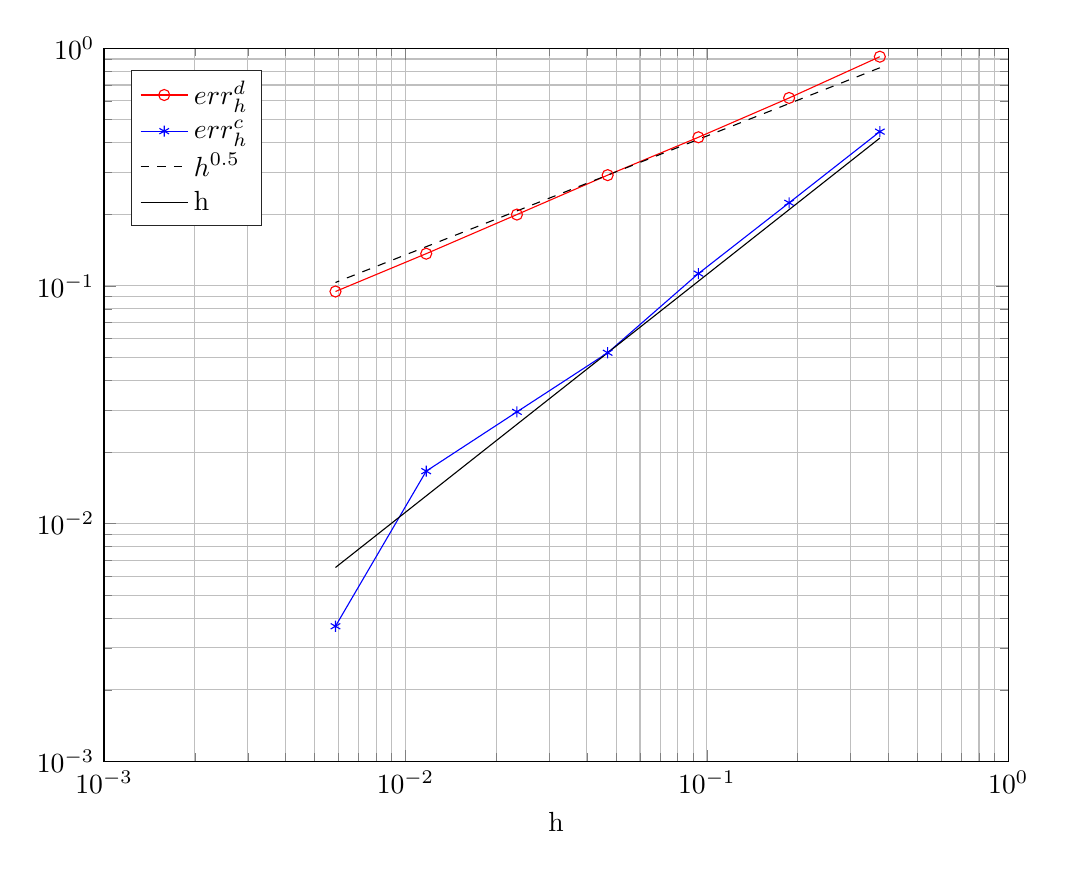
\begin{tikzpicture}

\begin{axis}[%
width=4.521in,
height=3.566in,
at={(0.758in,0.481in)},
scale only axis,
xmode=log,
xmin=0.001,
xmax=1,
xminorticks=true,
xlabel={h},
xmajorgrids,
xminorgrids,
ymode=log,
ymin=0.001,
ymax=1,
yminorticks=true,
ymajorgrids,
yminorgrids,
axis background/.style={fill=white},
legend style={at={(0.03,0.97)},anchor=north west,legend cell align=left,align=left,draw=white!15!black}
]
\addplot [color=red,solid,mark=o,mark options={solid}]
  table[row sep=crcr]{%
0.375	0.920558951920583\\
0.1875	0.617333951920583\\
0.09375	0.421846451920583\\
0.046875	0.292363639420583\\
0.0234375	0.199588639420583\\
0.01171875	0.136614420670583\\
0.005859375	0.0947198894205827\\
};
\addlegendentry{$\text{err}_\text{h}^\text{d}$};

\addplot [color=blue,solid,mark=asterisk,mark options={solid}]
  table[row sep=crcr]{%
0.375	0.445546451920583\\
0.1875	0.223658951920583\\
0.09375	0.112677701920583\\
0.046875	0.0523214519205826\\
0.0234375	0.0295214519205826\\
0.01171875	0.0166261394205827\\
0.005859375	0.00370153004558271\\
};
\addlegendentry{$\text{err}_\text{h}^\text{c}$};

\addplot [color=black,dashed]
  table[row sep=crcr]{%
0.375	0.82692924802669\\
0.1875	0.584727278841165\\
0.09375	0.413464624013345\\
0.046875	0.292363639420583\\
0.0234375	0.206732312006673\\
0.01171875	0.146181819710291\\
0.005859375	0.103366156003336\\
};
\addlegendentry{$\text{h}^{\text{0.5}}$};

\addplot [color=black,solid]
  table[row sep=crcr]{%
0.375	0.418571615364661\\
0.1875	0.20928580768233\\
0.09375	0.104642903841165\\
0.046875	0.0523214519205826\\
0.0234375	0.0261607259602913\\
0.01171875	0.0130803629801456\\
0.005859375	0.00654018149007282\\
};
\addlegendentry{h};

\end{axis}
\end{tikzpicture}% }  
        \caption{Convergence of CEM and DEM.}
        \label{fig:ReflTwoD}
    \end{subfigure}
    \begin{subfigure}{0.49\linewidth}
        \centering
        \resizebox{1\linewidth}{!}{% This file was created by matlab2tikz.
%
%The latest updates can be retrieved from
%  http://www.mathworks.com/matlabcentral/fileexchange/22022-matlab2tikz-matlab2tikz
%where you can also make suggestions and rate matlab2tikz.
%
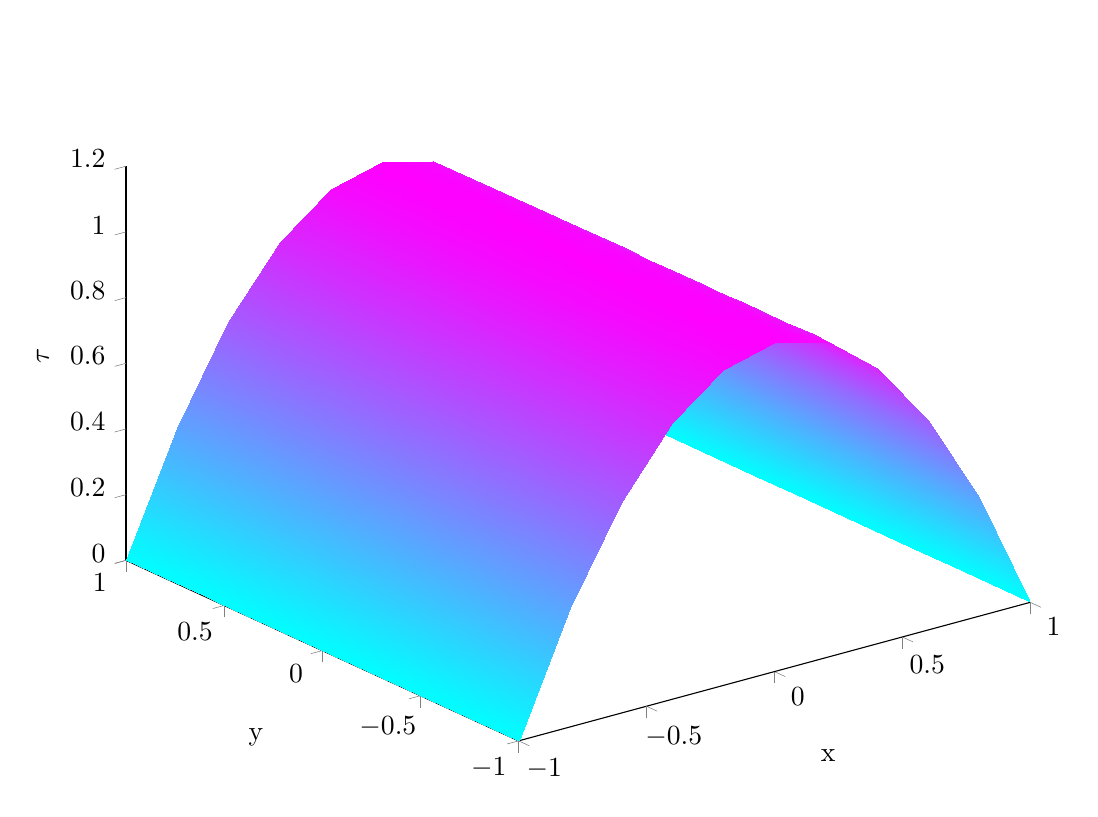
\begin{tikzpicture}

\begin{axis}[%
width=4.521in,
height=3.566in,
at={(0.758in,0.481in)},
scale only axis,
colormap={mymap}{[1pt] rgb(0pt)=(0,1,1); rgb(63pt)=(1,0,1)},
xmin=-1,
xmax=1,
tick align=outside,
xlabel={x},
ymin=-1,
ymax=1,
ylabel={y},
zmin=0,
zmax=1.2,
zlabel={$\tau$},
view={-37.5}{30},
axis background/.style={fill=white},
axis x line*=bottom,
axis y line*=left,
axis z line*=left
]

\addplot3[area legend,solid,table/row sep=crcr,patch,shader=interp,forget plot,patch table={%
0	1	2\\
3	4	5\\
6	7	8\\
9	10	11\\
12	13	14\\
15	16	17\\
18	19	20\\
21	22	23\\
24	25	26\\
27	28	29\\
30	31	32\\
33	34	35\\
36	37	38\\
39	40	41\\
42	43	44\\
45	46	47\\
48	49	50\\
51	52	53\\
54	55	56\\
57	58	59\\
60	61	62\\
63	64	65\\
66	67	68\\
69	70	71\\
72	73	74\\
75	76	77\\
78	79	80\\
81	82	83\\
84	85	86\\
87	88	89\\
90	91	92\\
93	94	95\\
96	97	98\\
99	100	101\\
102	103	104\\
105	106	107\\
108	109	110\\
111	112	113\\
114	115	116\\
117	118	119\\
120	121	122\\
123	124	125\\
126	127	128\\
129	130	131\\
132	133	134\\
135	136	137\\
138	139	140\\
141	142	143\\
144	145	146\\
147	148	149\\
150	151	152\\
153	154	155\\
156	157	158\\
159	160	161\\
162	163	164\\
165	166	167\\
168	169	170\\
171	172	173\\
174	175	176\\
177	178	179\\
180	181	182\\
183	184	185\\
186	187	188\\
189	190	191\\
192	193	194\\
195	196	197\\
198	199	200\\
201	202	203\\
204	205	206\\
207	208	209\\
210	211	212\\
213	214	215\\
216	217	218\\
219	220	221\\
222	223	224\\
225	226	227\\
228	229	230\\
231	232	233\\
234	235	236\\
237	238	239\\
240	241	242\\
243	244	245\\
246	247	248\\
249	250	251\\
252	253	254\\
255	256	257\\
258	259	260\\
261	262	263\\
264	265	266\\
267	268	269\\
270	271	272\\
273	274	275\\
276	277	278\\
279	280	281\\
282	283	284\\
285	286	287\\
288	289	290\\
291	292	293\\
294	295	296\\
297	298	299\\
300	301	302\\
303	304	305\\
306	307	308\\
309	310	311\\
312	313	314\\
315	316	317\\
318	319	320\\
321	322	323\\
324	325	326\\
327	328	329\\
330	331	332\\
333	334	335\\
336	337	338\\
339	340	341\\
342	343	344\\
345	346	347\\
348	349	350\\
351	352	353\\
354	355	356\\
357	358	359\\
360	361	362\\
363	364	365\\
366	367	368\\
369	370	371\\
372	373	374\\
375	376	377\\
378	379	380\\
381	382	383\\
384	385	386\\
387	388	389\\
390	391	392\\
393	394	395\\
396	397	398\\
399	400	401\\
402	403	404\\
405	406	407\\
408	409	410\\
411	412	413\\
414	415	416\\
417	418	419\\
420	421	422\\
423	424	425\\
426	427	428\\
429	430	431\\
432	433	434\\
435	436	437\\
438	439	440\\
441	442	443\\
444	445	446\\
447	448	449\\
450	451	452\\
453	454	455\\
456	457	458\\
459	460	461\\
462	463	464\\
465	466	467\\
468	469	470\\
471	472	473\\
474	475	476\\
477	478	479\\
480	481	482\\
483	484	485\\
486	487	488\\
489	490	491\\
492	493	494\\
495	496	497\\
498	499	500\\
501	502	503\\
504	505	506\\
507	508	509\\
510	511	512\\
513	514	515\\
516	517	518\\
519	520	521\\
522	523	524\\
525	526	527\\
528	529	530\\
531	532	533\\
534	535	536\\
537	538	539\\
540	541	542\\
543	544	545\\
546	547	548\\
549	550	551\\
552	553	554\\
555	556	557\\
558	559	560\\
561	562	563\\
564	565	566\\
567	568	569\\
570	571	572\\
573	574	575\\
576	577	578\\
579	580	581\\
582	583	584\\
585	586	587\\
588	589	590\\
591	592	593\\
594	595	596\\
597	598	599\\
600	601	602\\
603	604	605\\
606	607	608\\
609	610	611\\
612	613	614\\
615	616	617\\
618	619	620\\
621	622	623\\
624	625	626\\
627	628	629\\
630	631	632\\
633	634	635\\
636	637	638\\
639	640	641\\
642	643	644\\
645	646	647\\
648	649	650\\
651	652	653\\
654	655	656\\
657	658	659\\
660	661	662\\
663	664	665\\
666	667	668\\
669	670	671\\
672	673	674\\
675	676	677\\
678	679	680\\
681	682	683\\
684	685	686\\
687	688	689\\
690	691	692\\
693	694	695\\
696	697	698\\
699	700	701\\
702	703	704\\
705	706	707\\
708	709	710\\
711	712	713\\
714	715	716\\
717	718	719\\
720	721	722\\
723	724	725\\
726	727	728\\
729	730	731\\
732	733	734\\
735	736	737\\
738	739	740\\
741	742	743\\
744	745	746\\
747	748	749\\
750	751	752\\
753	754	755\\
756	757	758\\
759	760	761\\
762	763	764\\
765	766	767\\
768	769	770\\
771	772	773\\
774	775	776\\
777	778	779\\
780	781	782\\
783	784	785\\
786	787	788\\
789	790	791\\
792	793	794\\
795	796	797\\
798	799	800\\
801	802	803\\
804	805	806\\
807	808	809\\
810	811	812\\
813	814	815\\
816	817	818\\
819	820	821\\
822	823	824\\
825	826	827\\
828	829	830\\
831	832	833\\
834	835	836\\
837	838	839\\
840	841	842\\
843	844	845\\
846	847	848\\
849	850	851\\
852	853	854\\
855	856	857\\
858	859	860\\
861	862	863\\
864	865	866\\
867	868	869\\
870	871	872\\
873	874	875\\
876	877	878\\
879	880	881\\
882	883	884\\
885	886	887\\
888	889	890\\
891	892	893\\
894	895	896\\
897	898	899\\
900	901	902\\
903	904	905\\
906	907	908\\
909	910	911\\
912	913	914\\
915	916	917\\
918	919	920\\
921	922	923\\
924	925	926\\
927	928	929\\
930	931	932\\
933	934	935\\
}]
table[row sep=crcr, point meta=\thisrow{c}] {%
x	y	z	c\\
-0.8	1	0.360600789054301	0.360600789054301\\
-1	1	0	0\\
-0.870979864217162	0.874090623781756	0.239859277391115	0.239859277391115\\
-0.6	1	0.640491282159661	0.640491282159661\\
-0.8	1	0.360600789054301	0.360600789054301\\
-0.715759069893515	0.851783447512538	0.486496946106705	0.486496946106705\\
-0.4	1	0.841915538620754	0.841915538620754\\
-0.6	1	0.640491282159661	0.640491282159661\\
-0.553557227232278	0.85599352174284	0.692522390225689	0.692522390225689\\
-0.2	1	0.961730564647817	0.961730564647817\\
-0.4	1	0.841915538620754	0.841915538620754\\
-0.256371139537587	0.844436132195903	0.934083042087989	0.934083042087989\\
0	1	1.00284345596087	1.00284345596087\\
-0.2	1	0.961730564647817	0.961730564647817\\
-0.123171927132804	0.882407229449651	0.984158790678844	0.984158790678844\\
0.2	1	0.961368900240203	0.961368900240203\\
0	1	1.00284345596087	1.00284345596087\\
0.138576080047019	0.836444863570092	0.981193330437155	0.981193330437155\\
0.4	1	0.840760731727363	0.840760731727363\\
0.2	1	0.961368900240203	0.961368900240203\\
0.314746867281053	0.841650113118016	0.901147153165762	0.901147153165762\\
0.6	1	0.640360020804884	0.640360020804884\\
0.4	1	0.840760731727363	0.840760731727363\\
0.500557557249754	0.834821560479383	0.749201168032203	0.749201168032203\\
1	0.8	0	0\\
1	1	0	0\\
0.913245437763783	0.903908655259532	0.163805732451607	0.163805732451607\\
0.8	1	0.361493877531523	0.361493877531523\\
0.6	1	0.640360020804884	0.640360020804884\\
0.6908636124721	0.827426566529025	0.522063794642751	0.522063794642751\\
1	1	0	0\\
0.8	1	0.361493877531523	0.361493877531523\\
0.913245437763783	0.903908655259532	0.163805732451607	0.163805732451607\\
0.913245437763783	0.903908655259532	0.163805732451607	0.163805732451607\\
0.8	1	0.361493877531523	0.361493877531523\\
0.853111865010539	0.81689479082676	0.270990124964959	0.270990124964959\\
1	0.6	0	0\\
1	0.8	0	0\\
0.913257156072776	0.71766207885242	0.163230151401209	0.163230151401209\\
1	0.4	0	0\\
1	0.6	0	0\\
0.858172452446661	0.489687445107711	0.261682518030455	0.261682518030455\\
1	0.2	0	0\\
1	0.4	0	0\\
0.801876020058965	0.306586241275605	0.358544002692492	0.358544002692492\\
1	-0.2	0	0\\
1	0	0	0\\
0.842830738889788	-0.109162193087545	0.288668297301798	0.288668297301798\\
1	-0.4	0	0\\
1	-0.2	0	0\\
0.839553137409186	-0.294644298019888	0.294867736919447	0.294867736919447\\
1	-0.6	0	0\\
1	-0.4	0	0\\
0.825961266928206	-0.490102064147121	0.318608835409922	0.318608835409922\\
0.8	-1	0.361511288117814	0.361511288117814\\
1	-1	0	0\\
0.903543131650638	-0.913183857559471	0.179677948635493	0.179677948635493\\
1	-0.8	0	0\\
1	-0.6	0	0\\
0.822757598423982	-0.688930059869196	0.323681118411123	0.323681118411123\\
1	-1	0	0\\
1	-0.8	0	0\\
0.903543131650638	-0.913183857559471	0.179677948635493	0.179677948635493\\
0.903543131650638	-0.913183857559471	0.179677948635493	0.179677948635493\\
1	-0.8	0	0\\
0.815246907920555	-0.852962033044177	0.333913099068588	0.333913099068588\\
0.6	-1	0.640679825801503	0.640679825801503\\
0.8	-1	0.361511288117814	0.361511288117814\\
0.716262971529556	-0.913440138799354	0.483947882678644	0.483947882678644\\
0.4	-1	0.840779517817927	0.840779517817927\\
0.6	-1	0.640679825801503	0.640679825801503\\
0.486610676987292	-0.860815662729556	0.762434059022616	0.762434059022616\\
0.2	-1	0.960678353375381	0.960678353375381\\
0.4	-1	0.840779517817927	0.840779517817927\\
0.30415666992098	-0.806486553345674	0.909564391557416	0.909564391557416\\
-0.2	-1	0.961252352940462	0.961252352940462\\
0	-1	1.00122449995786	1.00122449995786\\
-0.108836774839956	-0.842631178463089	0.989101235372461	0.989101235372461\\
-0.4	-1	0.84054087387237	0.84054087387237\\
-0.2	-1	0.961252352940462	0.961252352940462\\
-0.295155054484333	-0.839202734226978	0.913311337508362	0.913311337508362\\
-0.6	-1	0.640424842543534	0.640424842543534\\
-0.4	-1	0.84054087387237	0.84054087387237\\
-0.491181950150036	-0.827450133500077	0.758860193106688	0.758860193106688\\
-1	-0.8	0	0\\
-1	-1	0	0\\
-0.913179600822541	-0.903978796898105	0.16404514787245	0.16404514787245\\
-0.8	-1	0.361717274493557	0.361717274493557\\
-0.6	-1	0.640424842543534	0.640424842543534\\
-0.689383148912005	-0.825669061227738	0.524631788972618	0.524631788972618\\
-1	-1	0	0\\
-0.8	-1	0.361717274493557	0.361717274493557\\
-0.913179600822541	-0.903978796898105	0.16404514787245	0.16404514787245\\
-0.913179600822541	-0.903978796898105	0.16404514787245	0.16404514787245\\
-0.8	-1	0.361717274493557	0.361717274493557\\
-0.852930471573381	-0.817084814175369	0.271555408139674	0.271555408139674\\
-1	-0.6	0	0\\
-1	-0.8	0	0\\
-0.913349182557632	-0.71824277938499	0.163203893325669	0.163203893325669\\
-1	-0.4	0	0\\
-1	-0.6	0	0\\
-0.858612569930114	-0.502582179815703	0.260853780386353	0.260853780386353\\
-1	-0.2	0	0\\
-1	-0.4	0	0\\
-0.875147249859378	-0.2495178793164	0.232618447603066	0.232618447603066\\
0.822757598423982	-0.688930059869196	0.323681118411123	0.323681118411123\\
1	-0.6	0	0\\
0.825961266928206	-0.490102064147121	0.318608835409922	0.318608835409922\\
-1	0.2	0	0\\
-1	0	0	0\\
-0.878430687062504	0.0687937548368703	0.225788638375186	0.225788638375186\\
-1	0.4	0	0\\
-1	0.2	0	0\\
-0.858638192546528	0.336283758462884	0.260561904995708	0.260561904995708\\
0.314746867281053	0.841650113118016	0.901147153165762	0.901147153165762\\
0.2	1	0.961368900240203	0.961368900240203\\
0.138576080047019	0.836444863570092	0.981193330437155	0.981193330437155\\
-1	0.6	0	0\\
-1	0.4	0	0\\
-0.81542002432126	0.514265339146589	0.336111582616146	0.336111582616146\\
-1	0	0	0\\
-1	-0.2	0	0\\
-0.849550627410001	-0.0857161204413969	0.278923893229734	0.278923893229734\\
-0.81542002432126	0.514265339146589	0.336111582616146	0.336111582616146\\
-1	0.4	0	0\\
-0.858638192546528	0.336283758462884	0.260561904995708	0.260561904995708\\
0	-1	1.00122449995786	1.00122449995786\\
0.2	-1	0.960678353375381	0.960678353375381\\
0.0842448278397462	-0.826656651009239	0.994216266348817	0.994216266348817\\
-0.295155054484333	-0.839202734226978	0.913311337508362	0.913311337508362\\
-0.2	-1	0.961252352940462	0.961252352940462\\
-0.108836774839956	-0.842631178463089	0.989101235372461	0.989101235372461\\
1	0	0	0\\
1	0.2	0	0\\
0.825000730866433	0.0840636812185947	0.319213914056299	0.319213914056299\\
0.839553137409186	-0.294644298019888	0.294867736919447	0.294867736919447\\
1	-0.2	0	0\\
0.842830738889788	-0.109162193087545	0.288668297301798	0.288668297301798\\
-0.421476522111469	0.76529746608585	0.822836734575626	0.822836734575626\\
-0.4	1	0.841915538620754	0.841915538620754\\
-0.553557227232278	0.85599352174284	0.692522390225689	0.692522390225689\\
-1	1	0	0\\
-1	0.8	0	0\\
-0.870979864217162	0.874090623781756	0.239859277391115	0.239859277391115\\
-1	0.8	0	0\\
-1	0.6	0	0\\
-0.838909094432717	0.717165597536304	0.297151196902934	0.297151196902934\\
-0.870979864217162	0.874090623781756	0.239859277391115	0.239859277391115\\
-1	0.8	0	0\\
-0.838909094432717	0.717165597536304	0.297151196902934	0.297151196902934\\
-0.689383148912005	-0.825669061227738	0.524631788972618	0.524631788972618\\
-0.6	-1	0.640424842543534	0.640424842543534\\
-0.491181950150036	-0.827450133500077	0.758860193106688	0.758860193106688\\
0.162899107774523	0.0782930267751429	0.974005215726172	0.974005215726172\\
-0.0145232187187818	0.0259493451768655	0.999205050761528	0.999205050761528\\
0.0995954131227801	-0.0711056079718885	0.988536281335325	0.988536281335325\\
0.6908636124721	0.827426566529025	0.522063794642751	0.522063794642751\\
0.6	1	0.640360020804884	0.640360020804884\\
0.500557557249754	0.834821560479383	0.749201168032203	0.749201168032203\\
-0.0437189086592884	-0.1794562797288	0.999407875924147	0.999407875924147\\
-0.0145232187187818	0.0259493451768655	0.999205050761528	0.999205050761528\\
-0.183666461200581	-0.0196981175980336	0.966126125617536	0.966126125617536\\
-0.183666461200581	-0.0196981175980336	0.966126125617536	0.966126125617536\\
-0.0145232187187818	0.0259493451768655	0.999205050761528	0.999205050761528\\
-0.143244730260345	0.15312684048721	0.979268321583401	0.979268321583401\\
-0.573742666641828	0.478792000601255	0.669119447374178	0.669119447374178\\
-0.435775856529045	0.402580883145608	0.808443041196626	0.808443041196626\\
-0.436448993108287	0.574739898722634	0.809399198789772	0.809399198789772\\
-0.777645420963466	0.191713474052978	0.396499642543184	0.396499642543184\\
-1	0.2	0	0\\
-0.878430687062504	0.0687937548368703	0.225788638375186	0.225788638375186\\
-0.308985524220196	-0.434191396690207	0.904638804118675	0.904638804118675\\
-0.44256229481138	-0.30475784338953	0.802616810542302	0.802616810542302\\
-0.504626867096141	-0.476494146294975	0.745183530905945	0.745183530905945\\
0.30415666992098	-0.806486553345674	0.909564391557416	0.909564391557416\\
0.4	-1	0.840779517817927	0.840779517817927\\
0.486610676987292	-0.860815662729556	0.762434059022616	0.762434059022616\\
0.0893690793198263	-0.463478876426208	0.991825156767633	0.991825156767633\\
0.261928641455601	-0.488055957894452	0.931707123511754	0.931707123511754\\
0.2060410026947	-0.342035240885369	0.956193171406951	0.956193171406951\\
0.801876020058965	0.306586241275605	0.358544002692492	0.358544002692492\\
1	0.4	0	0\\
0.858172452446661	0.489687445107711	0.261682518030455	0.261682518030455\\
0.500557557249754	0.834821560479383	0.749201168032203	0.749201168032203\\
0.4	1	0.840760731727363	0.840760731727363\\
0.314746867281053	0.841650113118016	0.901147153165762	0.901147153165762\\
-0.0174658545926647	0.801898927302032	0.99866022482065	0.99866022482065\\
0	1	1.00284345596087	1.00284345596087\\
-0.123171927132804	0.882407229449651	0.984158790678844	0.984158790678844\\
0.629591208237007	0.150059132096618	0.6051616820519	0.6051616820519\\
0.464005364535939	0.260203010616371	0.784232155411903	0.784232155411903\\
0.457941066948159	0.074681360252563	0.78988104270503	0.78988104270503\\
-0.536183382478912	-0.125067364855863	0.713275708382721	0.713275708382721\\
-0.44256229481138	-0.30475784338953	0.802616810542302	0.802616810542302\\
-0.376489904228021	-0.187383275146088	0.856428557335802	0.856428557335802\\
0.825961266928206	-0.490102064147121	0.318608835409922	0.318608835409922\\
1	-0.4	0	0\\
0.839553137409186	-0.294644298019888	0.294867736919447	0.294867736919447\\
-0.491181950150036	-0.827450133500077	0.758860193106688	0.758860193106688\\
-0.4	-1	0.84054087387237	0.84054087387237\\
-0.295155054484333	-0.839202734226978	0.913311337508362	0.913311337508362\\
0.151932036409303	-0.636460365815934	0.977221024462473	0.977221024462473\\
0.261928641455601	-0.488055957894452	0.931707123511754	0.931707123511754\\
0.0893690793198263	-0.463478876426208	0.991825156767633	0.991825156767633\\
-0.31111533158028	-0.281732042536466	0.900823435305982	0.900823435305982\\
-0.241660277500026	-0.172513969577467	0.94104375303322	0.94104375303322\\
-0.376489904228021	-0.187383275146088	0.856428557335802	0.856428557335802\\
-0.796122724389227	-0.361886425045465	0.366578675558219	0.366578675558219\\
-0.695084883753552	-0.495926997595022	0.516155190250719	0.516155190250719\\
-0.617615903555302	-0.32670910304294	0.617618625951112	0.617618625951112\\
0.321736948673632	-0.218404805181936	0.896441155494337	0.896441155494337\\
0.149400916774043	-0.200302697508326	0.977903731157044	0.977903731157044\\
0.2060410026947	-0.342035240885369	0.956193171406951	0.956193171406951\\
0.459725917575231	0.478817132146761	0.790069031749911	0.790069031749911\\
0.464005364535939	0.260203010616371	0.784232155411903	0.784232155411903\\
0.609248416595618	0.336700564235885	0.627389109399426	0.627389109399426\\
-0.591992818593216	-0.654470500305776	0.650535288706925	0.650535288706925\\
-0.368952164395011	-0.646051178924541	0.865159771739089	0.865159771739089\\
-0.504626867096141	-0.476494146294975	0.745183530905945	0.745183530905945\\
0.646526572158138	-0.5892372548303	0.582412304645243	0.582412304645243\\
0.647783933105589	-0.365727428795828	0.581960543118186	0.581960543118186\\
0.453484147433517	-0.490455219207141	0.796343218935013	0.796343218935013\\
-0.8	1	0.360600789054301	0.360600789054301\\
-0.870979864217162	0.874090623781756	0.239859277391115	0.239859277391115\\
-0.715759069893515	0.851783447512538	0.486496946106705	0.486496946106705\\
-0.436448993108287	0.574739898722634	0.809399198789772	0.809399198789772\\
-0.435775856529045	0.402580883145608	0.808443041196626	0.808443041196626\\
-0.305196827885855	0.481941510996423	0.90497953192299	0.90497953192299\\
0.651531723544283	-0.800304145152872	0.575505329328998	0.575505329328998\\
0.6	-1	0.640679825801503	0.640679825801503\\
0.716262971529556	-0.913440138799354	0.483947882678644	0.483947882678644\\
0.651531723544283	-0.800304145152872	0.575505329328998	0.575505329328998\\
0.822757598423982	-0.688930059869196	0.323681118411123	0.323681118411123\\
0.646526572158138	-0.5892372548303	0.582412304645243	0.582412304645243\\
0.457941066948159	0.074681360252563	0.78988104270503	0.78988104270503\\
0.464005364535939	0.260203010616371	0.784232155411903	0.784232155411903\\
0.313359205867812	0.176240487473655	0.902314503372277	0.902314503372277\\
0.799426193403826	0.656174087711846	0.362051657334271	0.362051657334271\\
1	0.6	0	0\\
0.913257156072776	0.71766207885242	0.163230151401209	0.163230151401209\\
-0.800381152695487	-0.658205081403852	0.360847392154216	0.360847392154216\\
-1	-0.6	0	0\\
-0.913349182557632	-0.71824277938499	0.163203893325669	0.163203893325669\\
-0.800381152695487	-0.658205081403852	0.360847392154216	0.360847392154216\\
-0.689383148912005	-0.825669061227738	0.524631788972618	0.524631788972618\\
-0.591992818593216	-0.654470500305776	0.650535288706925	0.650535288706925\\
-0.131538906378604	0.468005506270669	0.983664863582035	0.983664863582035\\
0.0468419620052357	0.523978954343319	0.997787191997233	0.997787191997233\\
-0.0677763280124889	0.648507972991784	0.995475124095099	0.995475124095099\\
0.172508063347201	0.422930104621211	0.969801938072441	0.969801938072441\\
0.0468419620052357	0.523978954343319	0.997787191997233	0.997787191997233\\
0.0285171270359044	0.362157622648837	0.998839239472402	0.998839239472402\\
0.453484147433517	-0.490455219207141	0.796343218935013	0.796343218935013\\
0.261928641455601	-0.488055957894452	0.931707123511754	0.931707123511754\\
0.32991065048365	-0.623943472007708	0.890313737599109	0.890313737599109\\
0.0893690793198263	-0.463478876426208	0.991825156767633	0.991825156767633\\
-0.0468923144628943	-0.37201189317892	0.995910394811523	0.995910394811523\\
-0.0519572972000214	-0.516668038614571	0.995594579092236	0.995594579092236\\
0.801876020058965	0.306586241275605	0.358544002692492	0.358544002692492\\
0.687082418720278	0.487393175878324	0.527941640690478	0.527941640690478\\
0.609248416595618	0.336700564235885	0.627389109399426	0.627389109399426\\
0.457941066948159	0.074681360252563	0.78988104270503	0.78988104270503\\
0.386220146013541	-0.0691483215457924	0.849423624075885	0.849423624075885\\
0.521855887175084	-0.0613271652026621	0.726372020364078	0.726372020364078\\
0.0893728715906334	0.678554065055819	0.991650060061569	0.991650060061569\\
0.0468419620052357	0.523978954343319	0.997787191997233	0.997787191997233\\
0.193142943255321	0.563632036809665	0.961941048929927	0.961941048929927\\
-0.467792458521678	0.219937427890346	0.782141146605041	0.782141146605041\\
-0.435775856529045	0.402580883145608	0.808443041196626	0.808443041196626\\
-0.560240270361451	0.344844062180542	0.68427035594505	0.68427035594505\\
0.0172621493060368	0.196448852647962	0.999246071249523	0.999246071249523\\
0.167453556422288	0.263155683226473	0.971886930521425	0.971886930521425\\
0.0285171270359044	0.362157622648837	0.998839239472402	0.998839239472402\\
-0.777645420963466	0.191713474052978	0.396499642543184	0.396499642543184\\
-0.617913717697813	0.079971000861777	0.618367749736385	0.618367749736385\\
-0.624616411644707	0.242665578371416	0.608546275201191	0.608546275201191\\
-0.536183382478912	-0.125067364855863	0.713275708382721	0.713275708382721\\
-0.617913717697813	0.079971000861777	0.618367749736385	0.618367749736385\\
-0.699519166874299	-0.0584145433376073	0.509307508178047	0.509307508178047\\
-0.421476522111469	0.76529746608585	0.822836734575626	0.822836734575626\\
-0.629666025324687	0.659481894250005	0.607552332385808	0.607552332385808\\
-0.436448993108287	0.574739898722634	0.809399198789772	0.809399198789772\\
-0.467792458521678	0.219937427890346	0.782141146605041	0.782141146605041\\
-0.617913717697813	0.079971000861777	0.618367749736385	0.618367749736385\\
-0.456541297467842	0.0462574378515442	0.789805427179391	0.789805427179391\\
-0.796122724389227	-0.361886425045465	0.366578675558219	0.366578675558219\\
-1	-0.4	0	0\\
-0.858612569930114	-0.502582179815703	0.260853780386353	0.260853780386353\\
0.30415666992098	-0.806486553345674	0.909564391557416	0.909564391557416\\
0.478214140797659	-0.695585476223675	0.771792139744435	0.771792139744435\\
0.32991065048365	-0.623943472007708	0.890313737599109	0.890313737599109\\
-0.350427977113875	-0.0568798710953585	0.877309622147461	0.877309622147461\\
-0.241660277500026	-0.172513969577467	0.94104375303322	0.94104375303322\\
-0.183666461200581	-0.0196981175980336	0.966126125617536	0.966126125617536\\
0.521855887175084	-0.0613271652026621	0.726372020364078	0.726372020364078\\
0.386220146013541	-0.0691483215457924	0.849423624075885	0.849423624075885\\
0.456651668322266	-0.168447833276863	0.789344615416974	0.789344615416974\\
-0.256371139537587	0.844436132195903	0.934083042087989	0.934083042087989\\
-0.251840934393812	0.65073582839654	0.937938137234837	0.937938137234837\\
-0.14310781983293	0.765817634248709	0.978490665753227	0.978490665753227\\
1	0.8	0	0\\
0.913245437763783	0.903908655259532	0.163805732451607	0.163805732451607\\
0.853111865010539	0.81689479082676	0.270990124964959	0.270990124964959\\
-0.131538906378604	0.468005506270669	0.983664863582035	0.983664863582035\\
-0.0999792356165469	0.29750658388758	0.988482208418077	0.988482208418077\\
0.0285171270359044	0.362157622648837	0.998839239472402	0.998839239472402\\
0.799426193403826	0.656174087711846	0.362051657334271	0.362051657334271\\
0.687082418720278	0.487393175878324	0.527941640690478	0.527941640690478\\
0.858172452446661	0.489687445107711	0.261682518030455	0.261682518030455\\
0.239679041234336	-0.0747988778282174	0.941281910369404	0.941281910369404\\
0.386220146013541	-0.0691483215457924	0.849423624075885	0.849423624075885\\
0.312829618686655	0.0361464359017708	0.900687642984663	0.900687642984663\\
0.651531723544283	-0.800304145152872	0.575505329328998	0.575505329328998\\
0.478214140797659	-0.695585476223675	0.771792139744435	0.771792139744435\\
0.486610676987292	-0.860815662729556	0.762434059022616	0.762434059022616\\
-0.0437189086592884	-0.1794562797288	0.999407875924147	0.999407875924147\\
-0.0468923144628943	-0.37201189317892	0.995910394811523	0.995910394811523\\
0.0706839927525276	-0.312287735493971	0.992873684588063	0.992873684588063\\
-0.617615903555302	-0.32670910304294	0.617618625951112	0.617618625951112\\
-0.695084883753552	-0.495926997595022	0.516155190250719	0.516155190250719\\
-0.504626867096141	-0.476494146294975	0.745183530905945	0.745183530905945\\
-0.308985524220196	-0.434191396690207	0.904638804118675	0.904638804118675\\
-0.368952164395011	-0.646051178924541	0.865159771739089	0.865159771739089\\
-0.188699779816531	-0.572089273359516	0.965016575917867	0.965016575917867\\
0.467892646677106	-0.300972929247376	0.780325884507073	0.780325884507073\\
0.647783933105589	-0.365727428795828	0.581960543118186	0.581960543118186\\
0.581538749766835	-0.190353470678335	0.659656229626338	0.659656229626338\\
0.321736948673632	-0.218404805181936	0.896441155494337	0.896441155494337\\
0.386220146013541	-0.0691483215457924	0.849423624075885	0.849423624075885\\
0.239679041234336	-0.0747988778282174	0.941281910369404	0.941281910369404\\
0.6908636124721	0.827426566529025	0.522063794642751	0.522063794642751\\
0.500557557249754	0.834821560479383	0.749201168032203	0.749201168032203\\
0.590963022235164	0.660549521945042	0.650593507260515	0.650593507260515\\
0.590963022235164	0.660549521945042	0.650593507260515	0.650593507260515\\
0.500557557249754	0.834821560479383	0.749201168032203	0.749201168032203\\
0.404778435204039	0.681910640519122	0.835501931894581	0.835501931894581\\
-0.838909094432717	0.717165597536304	0.297151196902934	0.297151196902934\\
-1	0.6	0	0\\
-0.81542002432126	0.514265339146589	0.336111582616146	0.336111582616146\\
-0.573742666641828	0.478792000601255	0.669119447374178	0.669119447374178\\
-0.629666025324687	0.659481894250005	0.607552332385808	0.607552332385808\\
-0.67998691843914	0.507882653342416	0.534583174440857	0.534583174440857\\
-1	-0.8	0	0\\
-0.913179600822541	-0.903978796898105	0.16404514787245	0.16404514787245\\
-0.852930471573381	-0.817084814175369	0.271555408139674	0.271555408139674\\
-0.491181950150036	-0.827450133500077	0.758860193106688	0.758860193106688\\
-0.368952164395011	-0.646051178924541	0.865159771739089	0.865159771739089\\
-0.591992818593216	-0.654470500305776	0.650535288706925	0.650535288706925\\
0.590963022235164	0.660549521945042	0.650593507260515	0.650593507260515\\
0.687082418720278	0.487393175878324	0.527941640690478	0.527941640690478\\
0.799426193403826	0.656174087711846	0.362051657334271	0.362051657334271\\
0.6908636124721	0.827426566529025	0.522063794642751	0.522063794642751\\
0.590963022235164	0.660549521945042	0.650593507260515	0.650593507260515\\
0.799426193403826	0.656174087711846	0.362051657334271	0.362051657334271\\
0.8	-1	0.361511288117814	0.361511288117814\\
0.903543131650638	-0.913183857559471	0.179677948635493	0.179677948635493\\
0.815246907920555	-0.852962033044177	0.333913099068588	0.333913099068588\\
0.825961266928206	-0.490102064147121	0.318608835409922	0.318608835409922\\
0.647783933105589	-0.365727428795828	0.581960543118186	0.581960543118186\\
0.646526572158138	-0.5892372548303	0.582412304645243	0.582412304645243\\
-0.188699779816531	-0.572089273359516	0.965016575917867	0.965016575917867\\
-0.368952164395011	-0.646051178924541	0.865159771739089	0.865159771739089\\
-0.201012514379659	-0.715085349646872	0.959262206950445	0.959262206950445\\
-0.536183382478912	-0.125067364855863	0.713275708382721	0.713275708382721\\
-0.729105054552535	-0.200822554621074	0.468604207302521	0.468604207302521\\
-0.617615903555302	-0.32670910304294	0.617618625951112	0.617618625951112\\
0.581538749766835	-0.190353470678335	0.659656229626338	0.659656229626338\\
0.647783933105589	-0.365727428795828	0.581960543118186	0.581960543118186\\
0.717419694116031	-0.201076983778939	0.482601983187922	0.482601983187922\\
0.151932036409303	-0.636460365815934	0.977221024462473	0.977221024462473\\
0.30415666992098	-0.806486553345674	0.909564391557416	0.909564391557416\\
0.32991065048365	-0.623943472007708	0.890313737599109	0.890313737599109\\
-0.0519572972000214	-0.516668038614571	0.995594579092236	0.995594579092236\\
-0.0468923144628943	-0.37201189317892	0.995910394811523	0.995910394811523\\
-0.156991111184629	-0.442497792882714	0.973539255645371	0.973539255645371\\
-0.31111533158028	-0.281732042536466	0.900823435305982	0.900823435305982\\
-0.308985524220196	-0.434191396690207	0.904638804118675	0.904638804118675\\
-0.185241010817594	-0.314270126024311	0.964509156836044	0.964509156836044\\
-0.467792458521678	0.219937427890346	0.782141146605041	0.782141146605041\\
-0.311591314295825	0.109324344546677	0.902213627361649	0.902213627361649\\
-0.270562051272334	0.305759011517556	0.927678927371092	0.927678927371092\\
0.162899107774523	0.0782930267751429	0.974005215726172	0.974005215726172\\
0.167453556422288	0.263155683226473	0.971886930521425	0.971886930521425\\
0.0172621493060368	0.196448852647962	0.999246071249523	0.999246071249523\\
0.629591208237007	0.150059132096618	0.6051616820519	0.6051616820519\\
0.801876020058965	0.306586241275605	0.358544002692492	0.358544002692492\\
0.609248416595618	0.336700564235885	0.627389109399426	0.627389109399426\\
0.314746867281053	0.841650113118016	0.901147153165762	0.901147153165762\\
0.243215438556557	0.696935801995676	0.940661157524487	0.940661157524487\\
0.404778435204039	0.681910640519122	0.835501931894581	0.835501931894581\\
-0.421476522111469	0.76529746608585	0.822836734575626	0.822836734575626\\
-0.251840934393812	0.65073582839654	0.937938137234837	0.937938137234837\\
-0.256371139537587	0.844436132195903	0.934083042087989	0.934083042087989\\
0.404778435204039	0.681910640519122	0.835501931894581	0.835501931894581\\
0.243215438556557	0.696935801995676	0.940661157524487	0.940661157524487\\
0.318221535321866	0.579996560046282	0.897713493052954	0.897713493052954\\
0.581538749766835	-0.190353470678335	0.659656229626338	0.659656229626338\\
0.671060117555799	-0.0425238644998574	0.548727835348561	0.548727835348561\\
0.521855887175084	-0.0613271652026621	0.726372020364078	0.726372020364078\\
0.842830738889788	-0.109162193087545	0.288668297301798	0.288668297301798\\
1	0	0	0\\
0.825000730866433	0.0840636812185947	0.319213914056299	0.319213914056299\\
-0.188699779816531	-0.572089273359516	0.965016575917867	0.965016575917867\\
-0.0400681817402094	-0.67007462624905	0.999631870493906	0.999631870493906\\
-0.0519572972000214	-0.516668038614571	0.995594579092236	0.995594579092236\\
-0.108836774839956	-0.842631178463089	0.989101235372461	0.989101235372461\\
0	-1	1.00122449995786	1.00122449995786\\
0.0842448278397462	-0.826656651009239	0.994216266348817	0.994216266348817\\
-0.838909094432717	0.717165597536304	0.297151196902934	0.297151196902934\\
-0.629666025324687	0.659481894250005	0.607552332385808	0.607552332385808\\
-0.715759069893515	0.851783447512538	0.486496946106705	0.486496946106705\\
-0.131538906378604	0.468005506270669	0.983664863582035	0.983664863582035\\
-0.251840934393812	0.65073582839654	0.937938137234837	0.937938137234837\\
-0.305196827885855	0.481941510996423	0.90497953192299	0.90497953192299\\
-0.573742666641828	0.478792000601255	0.669119447374178	0.669119447374178\\
-0.698784277302622	0.374550558446254	0.511260012699424	0.511260012699424\\
-0.560240270361451	0.344844062180542	0.68427035594505	0.68427035594505\\
-0.849550627410001	-0.0857161204413969	0.278923893229734	0.278923893229734\\
-1	-0.2	0	0\\
-0.875147249859378	-0.2495178793164	0.232618447603066	0.232618447603066\\
0.629591208237007	0.150059132096618	0.6051616820519	0.6051616820519\\
0.671060117555799	-0.0425238644998574	0.548727835348561	0.548727835348561\\
0.825000730866433	0.0840636812185947	0.319213914056299	0.319213914056299\\
0.647783933105589	-0.365727428795828	0.581960543118186	0.581960543118186\\
0.825961266928206	-0.490102064147121	0.318608835409922	0.318608835409922\\
0.839553137409186	-0.294644298019888	0.294867736919447	0.294867736919447\\
0.151932036409303	-0.636460365815934	0.977221024462473	0.977221024462473\\
-0.0400681817402094	-0.67007462624905	0.999631870493906	0.999631870493906\\
0.0842448278397462	-0.826656651009239	0.994216266348817	0.994216266348817\\
-0.368952164395011	-0.646051178924541	0.865159771739089	0.865159771739089\\
-0.491181950150036	-0.827450133500077	0.758860193106688	0.758860193106688\\
-0.295155054484333	-0.839202734226978	0.913311337508362	0.913311337508362\\
-0.849550627410001	-0.0857161204413969	0.278923893229734	0.278923893229734\\
-0.729105054552535	-0.200822554621074	0.468604207302521	0.468604207302521\\
-0.699519166874299	-0.0584145433376073	0.509307508178047	0.509307508178047\\
-0.270562051272334	0.305759011517556	0.927678927371092	0.927678927371092\\
-0.311591314295825	0.109324344546677	0.902213627361649	0.902213627361649\\
-0.143244730260345	0.15312684048721	0.979268321583401	0.979268321583401\\
-0.44256229481138	-0.30475784338953	0.802616810542302	0.802616810542302\\
-0.308985524220196	-0.434191396690207	0.904638804118675	0.904638804118675\\
-0.31111533158028	-0.281732042536466	0.900823435305982	0.900823435305982\\
-0.251840934393812	0.65073582839654	0.937938137234837	0.937938137234837\\
-0.421476522111469	0.76529746608585	0.822836734575626	0.822836734575626\\
-0.436448993108287	0.574739898722634	0.809399198789772	0.809399198789772\\
-0.0437189086592884	-0.1794562797288	0.999407875924147	0.999407875924147\\
0.149400916774043	-0.200302697508326	0.977903731157044	0.977903731157044\\
0.0995954131227801	-0.0711056079718885	0.988536281335325	0.988536281335325\\
0.459725917575231	0.478817132146761	0.790069031749911	0.790069031749911\\
0.29046632350991	0.478227595927983	0.914756552949991	0.914756552949991\\
0.311159739978053	0.346682633914339	0.903869398356384	0.903869398356384\\
-0.695084883753552	-0.495926997595022	0.516155190250719	0.516155190250719\\
-0.800381152695487	-0.658205081403852	0.360847392154216	0.360847392154216\\
-0.591992818593216	-0.654470500305776	0.650535288706925	0.650535288706925\\
-0.689383148912005	-0.825669061227738	0.524631788972618	0.524631788972618\\
-0.491181950150036	-0.827450133500077	0.758860193106688	0.758860193106688\\
-0.591992818593216	-0.654470500305776	0.650535288706925	0.650535288706925\\
0.478214140797659	-0.695585476223675	0.771792139744435	0.771792139744435\\
0.651531723544283	-0.800304145152872	0.575505329328998	0.575505329328998\\
0.646526572158138	-0.5892372548303	0.582412304645243	0.582412304645243\\
0.822757598423982	-0.688930059869196	0.323681118411123	0.323681118411123\\
0.825961266928206	-0.490102064147121	0.318608835409922	0.318608835409922\\
0.646526572158138	-0.5892372548303	0.582412304645243	0.582412304645243\\
-0.777645420963466	0.191713474052978	0.396499642543184	0.396499642543184\\
-0.698784277302622	0.374550558446254	0.511260012699424	0.511260012699424\\
-0.858638192546528	0.336283758462884	0.260561904995708	0.260561904995708\\
-0.629666025324687	0.659481894250005	0.607552332385808	0.607552332385808\\
-0.838909094432717	0.717165597536304	0.297151196902934	0.297151196902934\\
-0.81542002432126	0.514265339146589	0.336111582616146	0.336111582616146\\
-0.870979864217162	0.874090623781756	0.239859277391115	0.239859277391115\\
-0.838909094432717	0.717165597536304	0.297151196902934	0.297151196902934\\
-0.715759069893515	0.851783447512538	0.486496946106705	0.486496946106705\\
-0.715759069893515	0.851783447512538	0.486496946106705	0.486496946106705\\
-0.629666025324687	0.659481894250005	0.607552332385808	0.607552332385808\\
-0.553557227232278	0.85599352174284	0.692522390225689	0.692522390225689\\
-0.44256229481138	-0.30475784338953	0.802616810542302	0.802616810542302\\
-0.536183382478912	-0.125067364855863	0.713275708382721	0.713275708382721\\
-0.617615903555302	-0.32670910304294	0.617618625951112	0.617618625951112\\
-0.800381152695487	-0.658205081403852	0.360847392154216	0.360847392154216\\
-0.695084883753552	-0.495926997595022	0.516155190250719	0.516155190250719\\
-0.858612569930114	-0.502582179815703	0.260853780386353	0.260853780386353\\
-0.698784277302622	0.374550558446254	0.511260012699424	0.511260012699424\\
-0.777645420963466	0.191713474052978	0.396499642543184	0.396499642543184\\
-0.624616411644707	0.242665578371416	0.608546275201191	0.608546275201191\\
-0.81542002432126	0.514265339146589	0.336111582616146	0.336111582616146\\
-0.698784277302622	0.374550558446254	0.511260012699424	0.511260012699424\\
-0.67998691843914	0.507882653342416	0.534583174440857	0.534583174440857\\
-0.617913717697813	0.079971000861777	0.618367749736385	0.618367749736385\\
-0.777645420963466	0.191713474052978	0.396499642543184	0.396499642543184\\
-0.764656987373661	0.0391649423298058	0.413241553417644	0.413241553417644\\
-0.796122724389227	-0.361886425045465	0.366578675558219	0.366578675558219\\
-0.729105054552535	-0.200822554621074	0.468604207302521	0.468604207302521\\
-0.875147249859378	-0.2495178793164	0.232618447603066	0.232618447603066\\
0.321736948673632	-0.218404805181936	0.896441155494337	0.896441155494337\\
0.467892646677106	-0.300972929247376	0.780325884507073	0.780325884507073\\
0.456651668322266	-0.168447833276863	0.789344615416974	0.789344615416974\\
0.842830738889788	-0.109162193087545	0.288668297301798	0.288668297301798\\
0.671060117555799	-0.0425238644998574	0.548727835348561	0.548727835348561\\
0.717419694116031	-0.201076983778939	0.482601983187922	0.482601983187922\\
-0.185241010817594	-0.314270126024311	0.964509156836044	0.964509156836044\\
-0.308985524220196	-0.434191396690207	0.904638804118675	0.904638804118675\\
-0.156991111184629	-0.442497792882714	0.973539255645371	0.973539255645371\\
-0.108836774839956	-0.842631178463089	0.989101235372461	0.989101235372461\\
-0.0400681817402094	-0.67007462624905	0.999631870493906	0.999631870493906\\
-0.201012514379659	-0.715085349646872	0.959262206950445	0.959262206950445\\
0.2	-1	0.960678353375381	0.960678353375381\\
0.30415666992098	-0.806486553345674	0.909564391557416	0.909564391557416\\
0.0842448278397462	-0.826656651009239	0.994216266348817	0.994216266348817\\
-0.368952164395011	-0.646051178924541	0.865159771739089	0.865159771739089\\
-0.295155054484333	-0.839202734226978	0.913311337508362	0.913311337508362\\
-0.201012514379659	-0.715085349646872	0.959262206950445	0.959262206950445\\
1	0.2	0	0\\
0.801876020058965	0.306586241275605	0.358544002692492	0.358544002692492\\
0.825000730866433	0.0840636812185947	0.319213914056299	0.319213914056299\\
0.647783933105589	-0.365727428795828	0.581960543118186	0.581960543118186\\
0.839553137409186	-0.294644298019888	0.294867736919447	0.294867736919447\\
0.717419694116031	-0.201076983778939	0.482601983187922	0.482601983187922\\
0.459725917575231	0.478817132146761	0.790069031749911	0.790069031749911\\
0.590963022235164	0.660549521945042	0.650593507260515	0.650593507260515\\
0.404778435204039	0.681910640519122	0.835501931894581	0.835501931894581\\
0.172508063347201	0.422930104621211	0.969801938072441	0.969801938072441\\
0.29046632350991	0.478227595927983	0.914756552949991	0.914756552949991\\
0.193142943255321	0.563632036809665	0.961941048929927	0.961941048929927\\
-0.368952164395011	-0.646051178924541	0.865159771739089	0.865159771739089\\
-0.308985524220196	-0.434191396690207	0.904638804118675	0.904638804118675\\
-0.504626867096141	-0.476494146294975	0.745183530905945	0.745183530905945\\
-0.729105054552535	-0.200822554621074	0.468604207302521	0.468604207302521\\
-0.796122724389227	-0.361886425045465	0.366578675558219	0.366578675558219\\
-0.617615903555302	-0.32670910304294	0.617618625951112	0.617618625951112\\
0.687082418720278	0.487393175878324	0.527941640690478	0.527941640690478\\
0.801876020058965	0.306586241275605	0.358544002692492	0.358544002692492\\
0.858172452446661	0.489687445107711	0.261682518030455	0.261682518030455\\
1	0.6	0	0\\
0.799426193403826	0.656174087711846	0.362051657334271	0.362051657334271\\
0.858172452446661	0.489687445107711	0.261682518030455	0.261682518030455\\
0.478214140797659	-0.695585476223675	0.771792139744435	0.771792139744435\\
0.30415666992098	-0.806486553345674	0.909564391557416	0.909564391557416\\
0.486610676987292	-0.860815662729556	0.762434059022616	0.762434059022616\\
0.6	-1	0.640679825801503	0.640679825801503\\
0.651531723544283	-0.800304145152872	0.575505329328998	0.575505329328998\\
0.486610676987292	-0.860815662729556	0.762434059022616	0.762434059022616\\
0.453484147433517	-0.490455219207141	0.796343218935013	0.796343218935013\\
0.467892646677106	-0.300972929247376	0.780325884507073	0.780325884507073\\
0.342470518429332	-0.368426311537438	0.881038810494064	0.881038810494064\\
0.0995954131227801	-0.0711056079718885	0.988536281335325	0.988536281335325\\
0.149400916774043	-0.200302697508326	0.977903731157044	0.977903731157044\\
0.239679041234336	-0.0747988778282174	0.941281910369404	0.941281910369404\\
-0.8	-1	0.361717274493557	0.361717274493557\\
-0.689383148912005	-0.825669061227738	0.524631788972618	0.524631788972618\\
-0.852930471573381	-0.817084814175369	0.271555408139674	0.271555408139674\\
-0.689383148912005	-0.825669061227738	0.524631788972618	0.524631788972618\\
-0.800381152695487	-0.658205081403852	0.360847392154216	0.360847392154216\\
-0.852930471573381	-0.817084814175369	0.271555408139674	0.271555408139674\\
0.8	1	0.361493877531523	0.361493877531523\\
0.6908636124721	0.827426566529025	0.522063794642751	0.522063794642751\\
0.853111865010539	0.81689479082676	0.270990124964959	0.270990124964959\\
0.6908636124721	0.827426566529025	0.522063794642751	0.522063794642751\\
0.799426193403826	0.656174087711846	0.362051657334271	0.362051657334271\\
0.853111865010539	0.81689479082676	0.270990124964959	0.270990124964959\\
1	-0.8	0	0\\
0.822757598423982	-0.688930059869196	0.323681118411123	0.323681118411123\\
0.815246907920555	-0.852962033044177	0.333913099068588	0.333913099068588\\
0.822757598423982	-0.688930059869196	0.323681118411123	0.323681118411123\\
0.651531723544283	-0.800304145152872	0.575505329328998	0.575505329328998\\
0.815246907920555	-0.852962033044177	0.333913099068588	0.333913099068588\\
0.0172621493060368	0.196448852647962	0.999246071249523	0.999246071249523\\
-0.0999792356165469	0.29750658388758	0.988482208418077	0.988482208418077\\
-0.143244730260345	0.15312684048721	0.979268321583401	0.979268321583401\\
0.0893728715906334	0.678554065055819	0.991650060061569	0.991650060061569\\
-0.0174658545926647	0.801898927302032	0.99866022482065	0.99866022482065\\
-0.0677763280124889	0.648507972991784	0.995475124095099	0.995475124095099\\
0.30415666992098	-0.806486553345674	0.909564391557416	0.909564391557416\\
0.151932036409303	-0.636460365815934	0.977221024462473	0.977221024462473\\
0.0842448278397462	-0.826656651009239	0.994216266348817	0.994216266348817\\
-0.0400681817402094	-0.67007462624905	0.999631870493906	0.999631870493906\\
-0.108836774839956	-0.842631178463089	0.989101235372461	0.989101235372461\\
0.0842448278397462	-0.826656651009239	0.994216266348817	0.994216266348817\\
0.801876020058965	0.306586241275605	0.358544002692492	0.358544002692492\\
0.629591208237007	0.150059132096618	0.6051616820519	0.6051616820519\\
0.825000730866433	0.0840636812185947	0.319213914056299	0.319213914056299\\
0.671060117555799	-0.0425238644998574	0.548727835348561	0.548727835348561\\
0.842830738889788	-0.109162193087545	0.288668297301798	0.288668297301798\\
0.825000730866433	0.0840636812185947	0.319213914056299	0.319213914056299\\
0.342470518429332	-0.368426311537438	0.881038810494064	0.881038810494064\\
0.321736948673632	-0.218404805181936	0.896441155494337	0.896441155494337\\
0.2060410026947	-0.342035240885369	0.956193171406951	0.956193171406951\\
-0.241660277500026	-0.172513969577467	0.94104375303322	0.94104375303322\\
-0.0437189086592884	-0.1794562797288	0.999407875924147	0.999407875924147\\
-0.183666461200581	-0.0196981175980336	0.966126125617536	0.966126125617536\\
0.521855887175084	-0.0613271652026621	0.726372020364078	0.726372020364078\\
0.671060117555799	-0.0425238644998574	0.548727835348561	0.548727835348561\\
0.571417049604729	0.030140472637374	0.670966630526899	0.670966630526899\\
0.311159739978053	0.346682633914339	0.903869398356384	0.903869398356384\\
0.167453556422288	0.263155683226473	0.971886930521425	0.971886930521425\\
0.313359205867812	0.176240487473655	0.902314503372277	0.902314503372277\\
0.467892646677106	-0.300972929247376	0.780325884507073	0.780325884507073\\
0.321736948673632	-0.218404805181936	0.896441155494337	0.896441155494337\\
0.342470518429332	-0.368426311537438	0.881038810494064	0.881038810494064\\
-0.0519572972000214	-0.516668038614571	0.995594579092236	0.995594579092236\\
-0.0400681817402094	-0.67007462624905	0.999631870493906	0.999631870493906\\
0.0365478764267567	-0.57281221203974	0.995699582164407	0.995699582164407\\
0.687082418720278	0.487393175878324	0.527941640690478	0.527941640690478\\
0.590963022235164	0.660549521945042	0.650593507260515	0.650593507260515\\
0.459725917575231	0.478817132146761	0.790069031749911	0.790069031749911\\
0.193142943255321	0.563632036809665	0.961941048929927	0.961941048929927\\
0.29046632350991	0.478227595927983	0.914756552949991	0.914756552949991\\
0.318221535321866	0.579996560046282	0.897713493052954	0.897713493052954\\
-0.629666025324687	0.659481894250005	0.607552332385808	0.607552332385808\\
-0.573742666641828	0.478792000601255	0.669119447374178	0.669119447374178\\
-0.436448993108287	0.574739898722634	0.809399198789772	0.809399198789772\\
-0.270562051272334	0.305759011517556	0.927678927371092	0.927678927371092\\
-0.131538906378604	0.468005506270669	0.983664863582035	0.983664863582035\\
-0.305196827885855	0.481941510996423	0.90497953192299	0.90497953192299\\
0.647783933105589	-0.365727428795828	0.581960543118186	0.581960543118186\\
0.467892646677106	-0.300972929247376	0.780325884507073	0.780325884507073\\
0.453484147433517	-0.490455219207141	0.796343218935013	0.796343218935013\\
0.478214140797659	-0.695585476223675	0.771792139744435	0.771792139744435\\
0.646526572158138	-0.5892372548303	0.582412304645243	0.582412304645243\\
0.453484147433517	-0.490455219207141	0.796343218935013	0.796343218935013\\
-0.695084883753552	-0.495926997595022	0.516155190250719	0.516155190250719\\
-0.591992818593216	-0.654470500305776	0.650535288706925	0.650535288706925\\
-0.504626867096141	-0.476494146294975	0.745183530905945	0.745183530905945\\
-0.44256229481138	-0.30475784338953	0.802616810542302	0.802616810542302\\
-0.617615903555302	-0.32670910304294	0.617618625951112	0.617618625951112\\
-0.504626867096141	-0.476494146294975	0.745183530905945	0.745183530905945\\
0.500557557249754	0.834821560479383	0.749201168032203	0.749201168032203\\
0.314746867281053	0.841650113118016	0.901147153165762	0.901147153165762\\
0.404778435204039	0.681910640519122	0.835501931894581	0.835501931894581\\
0.29046632350991	0.478227595927983	0.914756552949991	0.914756552949991\\
0.459725917575231	0.478817132146761	0.790069031749911	0.790069031749911\\
0.318221535321866	0.579996560046282	0.897713493052954	0.897713493052954\\
0.464005364535939	0.260203010616371	0.784232155411903	0.784232155411903\\
0.629591208237007	0.150059132096618	0.6051616820519	0.6051616820519\\
0.609248416595618	0.336700564235885	0.627389109399426	0.627389109399426\\
0.687082418720278	0.487393175878324	0.527941640690478	0.527941640690478\\
0.459725917575231	0.478817132146761	0.790069031749911	0.790069031749911\\
0.609248416595618	0.336700564235885	0.627389109399426	0.627389109399426\\
-0.0677763280124889	0.648507972991784	0.995475124095099	0.995475124095099\\
-0.0174658545926647	0.801898927302032	0.99866022482065	0.99866022482065\\
-0.14310781983293	0.765817634248709	0.978490665753227	0.978490665753227\\
-0.4	1	0.841915538620754	0.841915538620754\\
-0.421476522111469	0.76529746608585	0.822836734575626	0.822836734575626\\
-0.256371139537587	0.844436132195903	0.934083042087989	0.934083042087989\\
-0.350427977113875	-0.0568798710953585	0.877309622147461	0.877309622147461\\
-0.311591314295825	0.109324344546677	0.902213627361649	0.902213627361649\\
-0.456541297467842	0.0462574378515442	0.789805427179391	0.789805427179391\\
-0.617913717697813	0.079971000861777	0.618367749736385	0.618367749736385\\
-0.536183382478912	-0.125067364855863	0.713275708382721	0.713275708382721\\
-0.456541297467842	0.0462574378515442	0.789805427179391	0.789805427179391\\
-0.435775856529045	0.402580883145608	0.808443041196626	0.808443041196626\\
-0.467792458521678	0.219937427890346	0.782141146605041	0.782141146605041\\
-0.270562051272334	0.305759011517556	0.927678927371092	0.927678927371092\\
-0.0999792356165469	0.29750658388758	0.988482208418077	0.988482208418077\\
-0.131538906378604	0.468005506270669	0.983664863582035	0.983664863582035\\
-0.270562051272334	0.305759011517556	0.927678927371092	0.927678927371092\\
0.0468419620052357	0.523978954343319	0.997787191997233	0.997787191997233\\
-0.131538906378604	0.468005506270669	0.983664863582035	0.983664863582035\\
0.0285171270359044	0.362157622648837	0.998839239472402	0.998839239472402\\
-0.0145232187187818	0.0259493451768655	0.999205050761528	0.999205050761528\\
0.162899107774523	0.0782930267751429	0.974005215726172	0.974005215726172\\
0.0172621493060368	0.196448852647962	0.999246071249523	0.999246071249523\\
-0.311591314295825	0.109324344546677	0.902213627361649	0.902213627361649\\
-0.350427977113875	-0.0568798710953585	0.877309622147461	0.877309622147461\\
-0.183666461200581	-0.0196981175980336	0.966126125617536	0.966126125617536\\
-0.0999792356165469	0.29750658388758	0.988482208418077	0.988482208418077\\
-0.270562051272334	0.305759011517556	0.927678927371092	0.927678927371092\\
-0.143244730260345	0.15312684048721	0.979268321583401	0.979268321583401\\
-0.617913717697813	0.079971000861777	0.618367749736385	0.618367749736385\\
-0.467792458521678	0.219937427890346	0.782141146605041	0.782141146605041\\
-0.624616411644707	0.242665578371416	0.608546275201191	0.608546275201191\\
-0.624616411644707	0.242665578371416	0.608546275201191	0.608546275201191\\
-0.467792458521678	0.219937427890346	0.782141146605041	0.782141146605041\\
-0.560240270361451	0.344844062180542	0.68427035594505	0.68427035594505\\
-0.251840934393812	0.65073582839654	0.937938137234837	0.937938137234837\\
-0.131538906378604	0.468005506270669	0.983664863582035	0.983664863582035\\
-0.0677763280124889	0.648507972991784	0.995475124095099	0.995475124095099\\
-0.2	1	0.961730564647817	0.961730564647817\\
-0.256371139537587	0.844436132195903	0.934083042087989	0.934083042087989\\
-0.123171927132804	0.882407229449651	0.984158790678844	0.984158790678844\\
0.467892646677106	-0.300972929247376	0.780325884507073	0.780325884507073\\
0.581538749766835	-0.190353470678335	0.659656229626338	0.659656229626338\\
0.456651668322266	-0.168447833276863	0.789344615416974	0.789344615416974\\
0.671060117555799	-0.0425238644998574	0.548727835348561	0.548727835348561\\
0.629591208237007	0.150059132096618	0.6051616820519	0.6051616820519\\
0.571417049604729	0.030140472637374	0.670966630526899	0.670966630526899\\
-0.308985524220196	-0.434191396690207	0.904638804118675	0.904638804118675\\
-0.188699779816531	-0.572089273359516	0.965016575917867	0.965016575917867\\
-0.156991111184629	-0.442497792882714	0.973539255645371	0.973539255645371\\
-0.0400681817402094	-0.67007462624905	0.999631870493906	0.999631870493906\\
0.151932036409303	-0.636460365815934	0.977221024462473	0.977221024462473\\
0.0365478764267567	-0.57281221203974	0.995699582164407	0.995699582164407\\
-1	-0.6	0	0\\
-0.800381152695487	-0.658205081403852	0.360847392154216	0.360847392154216\\
-0.858612569930114	-0.502582179815703	0.260853780386353	0.260853780386353\\
-0.695084883753552	-0.495926997595022	0.516155190250719	0.516155190250719\\
-0.796122724389227	-0.361886425045465	0.366578675558219	0.366578675558219\\
-0.858612569930114	-0.502582179815703	0.260853780386353	0.260853780386353\\
-1	0.2	0	0\\
-0.777645420963466	0.191713474052978	0.396499642543184	0.396499642543184\\
-0.858638192546528	0.336283758462884	0.260561904995708	0.260561904995708\\
-0.698784277302622	0.374550558446254	0.511260012699424	0.511260012699424\\
-0.81542002432126	0.514265339146589	0.336111582616146	0.336111582616146\\
-0.858638192546528	0.336283758462884	0.260561904995708	0.260561904995708\\
0	1	1.00284345596087	1.00284345596087\\
-0.0174658545926647	0.801898927302032	0.99866022482065	0.99866022482065\\
0.138576080047019	0.836444863570092	0.981193330437155	0.981193330437155\\
0.243215438556557	0.696935801995676	0.940661157524487	0.940661157524487\\
0.314746867281053	0.841650113118016	0.901147153165762	0.901147153165762\\
0.138576080047019	0.836444863570092	0.981193330437155	0.981193330437155\\
-0.729105054552535	-0.200822554621074	0.468604207302521	0.468604207302521\\
-0.536183382478912	-0.125067364855863	0.713275708382721	0.713275708382721\\
-0.699519166874299	-0.0584145433376073	0.509307508178047	0.509307508178047\\
-0.764656987373661	0.0391649423298058	0.413241553417644	0.413241553417644\\
-0.777645420963466	0.191713474052978	0.396499642543184	0.396499642543184\\
-0.878430687062504	0.0687937548368703	0.225788638375186	0.225788638375186\\
0.167453556422288	0.263155683226473	0.971886930521425	0.971886930521425\\
0.162899107774523	0.0782930267751429	0.974005215726172	0.974005215726172\\
0.313359205867812	0.176240487473655	0.902314503372277	0.902314503372277\\
0.464005364535939	0.260203010616371	0.784232155411903	0.784232155411903\\
0.459725917575231	0.478817132146761	0.790069031749911	0.790069031749911\\
0.311159739978053	0.346682633914339	0.903869398356384	0.903869398356384\\
0.311159739978053	0.346682633914339	0.903869398356384	0.903869398356384\\
0.29046632350991	0.478227595927983	0.914756552949991	0.914756552949991\\
0.172508063347201	0.422930104621211	0.969801938072441	0.969801938072441\\
0.167453556422288	0.263155683226473	0.971886930521425	0.971886930521425\\
0.311159739978053	0.346682633914339	0.903869398356384	0.903869398356384\\
0.172508063347201	0.422930104621211	0.969801938072441	0.969801938072441\\
-0.0437189086592884	-0.1794562797288	0.999407875924147	0.999407875924147\\
-0.241660277500026	-0.172513969577467	0.94104375303322	0.94104375303322\\
-0.185241010817594	-0.314270126024311	0.964509156836044	0.964509156836044\\
-0.350427977113875	-0.0568798710953585	0.877309622147461	0.877309622147461\\
-0.536183382478912	-0.125067364855863	0.713275708382721	0.713275708382721\\
-0.376489904228021	-0.187383275146088	0.856428557335802	0.856428557335802\\
0.313359205867812	0.176240487473655	0.902314503372277	0.902314503372277\\
0.162899107774523	0.0782930267751429	0.974005215726172	0.974005215726172\\
0.312829618686655	0.0361464359017708	0.900687642984663	0.900687642984663\\
-0.0145232187187818	0.0259493451768655	0.999205050761528	0.999205050761528\\
-0.0437189086592884	-0.1794562797288	0.999407875924147	0.999407875924147\\
0.0995954131227801	-0.0711056079718885	0.988536281335325	0.988536281335325\\
0.138576080047019	0.836444863570092	0.981193330437155	0.981193330437155\\
-0.0174658545926647	0.801898927302032	0.99866022482065	0.99866022482065\\
0.0893728715906334	0.678554065055819	0.991650060061569	0.991650060061569\\
0.243215438556557	0.696935801995676	0.940661157524487	0.940661157524487\\
0.138576080047019	0.836444863570092	0.981193330437155	0.981193330437155\\
0.0893728715906334	0.678554065055819	0.991650060061569	0.991650060061569\\
-1	0	0	0\\
-0.849550627410001	-0.0857161204413969	0.278923893229734	0.278923893229734\\
-0.878430687062504	0.0687937548368703	0.225788638375186	0.225788638375186\\
-0.849550627410001	-0.0857161204413969	0.278923893229734	0.278923893229734\\
-0.764656987373661	0.0391649423298058	0.413241553417644	0.413241553417644\\
-0.878430687062504	0.0687937548368703	0.225788638375186	0.225788638375186\\
-0.629666025324687	0.659481894250005	0.607552332385808	0.607552332385808\\
-0.421476522111469	0.76529746608585	0.822836734575626	0.822836734575626\\
-0.553557227232278	0.85599352174284	0.692522390225689	0.692522390225689\\
-0.6	1	0.640491282159661	0.640491282159661\\
-0.715759069893515	0.851783447512538	0.486496946106705	0.486496946106705\\
-0.553557227232278	0.85599352174284	0.692522390225689	0.692522390225689\\
0.671060117555799	-0.0425238644998574	0.548727835348561	0.548727835348561\\
0.581538749766835	-0.190353470678335	0.659656229626338	0.659656229626338\\
0.717419694116031	-0.201076983778939	0.482601983187922	0.482601983187922\\
0.839553137409186	-0.294644298019888	0.294867736919447	0.294867736919447\\
0.842830738889788	-0.109162193087545	0.288668297301798	0.288668297301798\\
0.717419694116031	-0.201076983778939	0.482601983187922	0.482601983187922\\
-0.0400681817402094	-0.67007462624905	0.999631870493906	0.999631870493906\\
-0.188699779816531	-0.572089273359516	0.965016575917867	0.965016575917867\\
-0.201012514379659	-0.715085349646872	0.959262206950445	0.959262206950445\\
-0.295155054484333	-0.839202734226978	0.913311337508362	0.913311337508362\\
-0.108836774839956	-0.842631178463089	0.989101235372461	0.989101235372461\\
-0.201012514379659	-0.715085349646872	0.959262206950445	0.959262206950445\\
-1	-0.4	0	0\\
-0.796122724389227	-0.361886425045465	0.366578675558219	0.366578675558219\\
-0.875147249859378	-0.2495178793164	0.232618447603066	0.232618447603066\\
-0.729105054552535	-0.200822554621074	0.468604207302521	0.468604207302521\\
-0.849550627410001	-0.0857161204413969	0.278923893229734	0.278923893229734\\
-0.875147249859378	-0.2495178793164	0.232618447603066	0.232618447603066\\
-0.852930471573381	-0.817084814175369	0.271555408139674	0.271555408139674\\
-0.800381152695487	-0.658205081403852	0.360847392154216	0.360847392154216\\
-0.913349182557632	-0.71824277938499	0.163203893325669	0.163203893325669\\
-1	-0.8	0	0\\
-0.852930471573381	-0.817084814175369	0.271555408139674	0.271555408139674\\
-0.913349182557632	-0.71824277938499	0.163203893325669	0.163203893325669\\
0.853111865010539	0.81689479082676	0.270990124964959	0.270990124964959\\
0.799426193403826	0.656174087711846	0.362051657334271	0.362051657334271\\
0.913257156072776	0.71766207885242	0.163230151401209	0.163230151401209\\
1	0.8	0	0\\
0.853111865010539	0.81689479082676	0.270990124964959	0.270990124964959\\
0.913257156072776	0.71766207885242	0.163230151401209	0.163230151401209\\
0.815246907920555	-0.852962033044177	0.333913099068588	0.333913099068588\\
0.651531723544283	-0.800304145152872	0.575505329328998	0.575505329328998\\
0.716262971529556	-0.913440138799354	0.483947882678644	0.483947882678644\\
0.8	-1	0.361511288117814	0.361511288117814\\
0.815246907920555	-0.852962033044177	0.333913099068588	0.333913099068588\\
0.716262971529556	-0.913440138799354	0.483947882678644	0.483947882678644\\
-0.629666025324687	0.659481894250005	0.607552332385808	0.607552332385808\\
-0.81542002432126	0.514265339146589	0.336111582616146	0.336111582616146\\
-0.67998691843914	0.507882653342416	0.534583174440857	0.534583174440857\\
-0.698784277302622	0.374550558446254	0.511260012699424	0.511260012699424\\
-0.573742666641828	0.478792000601255	0.669119447374178	0.669119447374178\\
-0.67998691843914	0.507882653342416	0.534583174440857	0.534583174440857\\
0.0706839927525276	-0.312287735493971	0.992873684588063	0.992873684588063\\
0.0893690793198263	-0.463478876426208	0.991825156767633	0.991825156767633\\
0.2060410026947	-0.342035240885369	0.956193171406951	0.956193171406951\\
0.261928641455601	-0.488055957894452	0.931707123511754	0.931707123511754\\
0.453484147433517	-0.490455219207141	0.796343218935013	0.796343218935013\\
0.342470518429332	-0.368426311537438	0.881038810494064	0.881038810494064\\
0.261928641455601	-0.488055957894452	0.931707123511754	0.931707123511754\\
0.151932036409303	-0.636460365815934	0.977221024462473	0.977221024462473\\
0.32991065048365	-0.623943472007708	0.890313737599109	0.890313737599109\\
0.478214140797659	-0.695585476223675	0.771792139744435	0.771792139744435\\
0.453484147433517	-0.490455219207141	0.796343218935013	0.796343218935013\\
0.32991065048365	-0.623943472007708	0.890313737599109	0.890313737599109\\
-0.123171927132804	0.882407229449651	0.984158790678844	0.984158790678844\\
-0.256371139537587	0.844436132195903	0.934083042087989	0.934083042087989\\
-0.14310781983293	0.765817634248709	0.978490665753227	0.978490665753227\\
0.0468419620052357	0.523978954343319	0.997787191997233	0.997787191997233\\
0.0893728715906334	0.678554065055819	0.991650060061569	0.991650060061569\\
-0.0677763280124889	0.648507972991784	0.995475124095099	0.995475124095099\\
-0.0145232187187818	0.0259493451768655	0.999205050761528	0.999205050761528\\
0.0172621493060368	0.196448852647962	0.999246071249523	0.999246071249523\\
-0.143244730260345	0.15312684048721	0.979268321583401	0.979268321583401\\
-0.311591314295825	0.109324344546677	0.902213627361649	0.902213627361649\\
-0.183666461200581	-0.0196981175980336	0.966126125617536	0.966126125617536\\
-0.143244730260345	0.15312684048721	0.979268321583401	0.979268321583401\\
-0.435775856529045	0.402580883145608	0.808443041196626	0.808443041196626\\
-0.573742666641828	0.478792000601255	0.669119447374178	0.669119447374178\\
-0.560240270361451	0.344844062180542	0.68427035594505	0.68427035594505\\
-0.698784277302622	0.374550558446254	0.511260012699424	0.511260012699424\\
-0.624616411644707	0.242665578371416	0.608546275201191	0.608546275201191\\
-0.560240270361451	0.344844062180542	0.68427035594505	0.68427035594505\\
0.386220146013541	-0.0691483215457924	0.849423624075885	0.849423624075885\\
0.457941066948159	0.074681360252563	0.78988104270503	0.78988104270503\\
0.312829618686655	0.0361464359017708	0.900687642984663	0.900687642984663\\
0.464005364535939	0.260203010616371	0.784232155411903	0.784232155411903\\
0.311159739978053	0.346682633914339	0.903869398356384	0.903869398356384\\
0.313359205867812	0.176240487473655	0.902314503372277	0.902314503372277\\
-0.251840934393812	0.65073582839654	0.937938137234837	0.937938137234837\\
-0.436448993108287	0.574739898722634	0.809399198789772	0.809399198789772\\
-0.305196827885855	0.481941510996423	0.90497953192299	0.90497953192299\\
-0.435775856529045	0.402580883145608	0.808443041196626	0.808443041196626\\
-0.270562051272334	0.305759011517556	0.927678927371092	0.927678927371092\\
-0.305196827885855	0.481941510996423	0.90497953192299	0.90497953192299\\
-0.311591314295825	0.109324344546677	0.902213627361649	0.902213627361649\\
-0.467792458521678	0.219937427890346	0.782141146605041	0.782141146605041\\
-0.456541297467842	0.0462574378515442	0.789805427179391	0.789805427179391\\
-0.536183382478912	-0.125067364855863	0.713275708382721	0.713275708382721\\
-0.350427977113875	-0.0568798710953585	0.877309622147461	0.877309622147461\\
-0.456541297467842	0.0462574378515442	0.789805427179391	0.789805427179391\\
-0.0468923144628943	-0.37201189317892	0.995910394811523	0.995910394811523\\
-0.0437189086592884	-0.1794562797288	0.999407875924147	0.999407875924147\\
-0.185241010817594	-0.314270126024311	0.964509156836044	0.964509156836044\\
-0.241660277500026	-0.172513969577467	0.94104375303322	0.94104375303322\\
-0.31111533158028	-0.281732042536466	0.900823435305982	0.900823435305982\\
-0.185241010817594	-0.314270126024311	0.964509156836044	0.964509156836044\\
0.149400916774043	-0.200302697508326	0.977903731157044	0.977903731157044\\
-0.0437189086592884	-0.1794562797288	0.999407875924147	0.999407875924147\\
0.0706839927525276	-0.312287735493971	0.992873684588063	0.992873684588063\\
-0.0468923144628943	-0.37201189317892	0.995910394811523	0.995910394811523\\
0.0893690793198263	-0.463478876426208	0.991825156767633	0.991825156767633\\
0.0706839927525276	-0.312287735493971	0.992873684588063	0.992873684588063\\
-0.241660277500026	-0.172513969577467	0.94104375303322	0.94104375303322\\
-0.350427977113875	-0.0568798710953585	0.877309622147461	0.877309622147461\\
-0.376489904228021	-0.187383275146088	0.856428557335802	0.856428557335802\\
-0.44256229481138	-0.30475784338953	0.802616810542302	0.802616810542302\\
-0.31111533158028	-0.281732042536466	0.900823435305982	0.900823435305982\\
-0.376489904228021	-0.187383275146088	0.856428557335802	0.856428557335802\\
-0.0999792356165469	0.29750658388758	0.988482208418077	0.988482208418077\\
0.0172621493060368	0.196448852647962	0.999246071249523	0.999246071249523\\
0.0285171270359044	0.362157622648837	0.998839239472402	0.998839239472402\\
0.167453556422288	0.263155683226473	0.971886930521425	0.971886930521425\\
0.172508063347201	0.422930104621211	0.969801938072441	0.969801938072441\\
0.0285171270359044	0.362157622648837	0.998839239472402	0.998839239472402\\
-0.764656987373661	0.0391649423298058	0.413241553417644	0.413241553417644\\
-0.849550627410001	-0.0857161204413969	0.278923893229734	0.278923893229734\\
-0.699519166874299	-0.0584145433376073	0.509307508178047	0.509307508178047\\
-0.617913717697813	0.079971000861777	0.618367749736385	0.618367749736385\\
-0.764656987373661	0.0391649423298058	0.413241553417644	0.413241553417644\\
-0.699519166874299	-0.0584145433376073	0.509307508178047	0.509307508178047\\
0.149400916774043	-0.200302697508326	0.977903731157044	0.977903731157044\\
0.321736948673632	-0.218404805181936	0.896441155494337	0.896441155494337\\
0.239679041234336	-0.0747988778282174	0.941281910369404	0.941281910369404\\
0.162899107774523	0.0782930267751429	0.974005215726172	0.974005215726172\\
0.0995954131227801	-0.0711056079718885	0.988536281335325	0.988536281335325\\
0.239679041234336	-0.0747988778282174	0.941281910369404	0.941281910369404\\
0.0468419620052357	0.523978954343319	0.997787191997233	0.997787191997233\\
0.172508063347201	0.422930104621211	0.969801938072441	0.969801938072441\\
0.193142943255321	0.563632036809665	0.961941048929927	0.961941048929927\\
0.243215438556557	0.696935801995676	0.940661157524487	0.940661157524487\\
0.0893728715906334	0.678554065055819	0.991650060061569	0.991650060061569\\
0.193142943255321	0.563632036809665	0.961941048929927	0.961941048929927\\
0.459725917575231	0.478817132146761	0.790069031749911	0.790069031749911\\
0.404778435204039	0.681910640519122	0.835501931894581	0.835501931894581\\
0.318221535321866	0.579996560046282	0.897713493052954	0.897713493052954\\
0.243215438556557	0.696935801995676	0.940661157524487	0.940661157524487\\
0.193142943255321	0.563632036809665	0.961941048929927	0.961941048929927\\
0.318221535321866	0.579996560046282	0.897713493052954	0.897713493052954\\
0.261928641455601	-0.488055957894452	0.931707123511754	0.931707123511754\\
0.342470518429332	-0.368426311537438	0.881038810494064	0.881038810494064\\
0.2060410026947	-0.342035240885369	0.956193171406951	0.956193171406951\\
0.149400916774043	-0.200302697508326	0.977903731157044	0.977903731157044\\
0.0706839927525276	-0.312287735493971	0.992873684588063	0.992873684588063\\
0.2060410026947	-0.342035240885369	0.956193171406951	0.956193171406951\\
0.386220146013541	-0.0691483215457924	0.849423624075885	0.849423624075885\\
0.321736948673632	-0.218404805181936	0.896441155494337	0.896441155494337\\
0.456651668322266	-0.168447833276863	0.789344615416974	0.789344615416974\\
0.581538749766835	-0.190353470678335	0.659656229626338	0.659656229626338\\
0.521855887175084	-0.0613271652026621	0.726372020364078	0.726372020364078\\
0.456651668322266	-0.168447833276863	0.789344615416974	0.789344615416974\\
-0.188699779816531	-0.572089273359516	0.965016575917867	0.965016575917867\\
-0.0519572972000214	-0.516668038614571	0.995594579092236	0.995594579092236\\
-0.156991111184629	-0.442497792882714	0.973539255645371	0.973539255645371\\
-0.0468923144628943	-0.37201189317892	0.995910394811523	0.995910394811523\\
-0.185241010817594	-0.314270126024311	0.964509156836044	0.964509156836044\\
-0.156991111184629	-0.442497792882714	0.973539255645371	0.973539255645371\\
0.629591208237007	0.150059132096618	0.6051616820519	0.6051616820519\\
0.457941066948159	0.074681360252563	0.78988104270503	0.78988104270503\\
0.571417049604729	0.030140472637374	0.670966630526899	0.670966630526899\\
0.457941066948159	0.074681360252563	0.78988104270503	0.78988104270503\\
0.521855887175084	-0.0613271652026621	0.726372020364078	0.726372020364078\\
0.571417049604729	0.030140472637374	0.670966630526899	0.670966630526899\\
0.151932036409303	-0.636460365815934	0.977221024462473	0.977221024462473\\
0.0893690793198263	-0.463478876426208	0.991825156767633	0.991825156767633\\
0.0365478764267567	-0.57281221203974	0.995699582164407	0.995699582164407\\
0.0893690793198263	-0.463478876426208	0.991825156767633	0.991825156767633\\
-0.0519572972000214	-0.516668038614571	0.995594579092236	0.995594579092236\\
0.0365478764267567	-0.57281221203974	0.995699582164407	0.995699582164407\\
-0.0174658545926647	0.801898927302032	0.99866022482065	0.99866022482065\\
-0.123171927132804	0.882407229449651	0.984158790678844	0.984158790678844\\
-0.14310781983293	0.765817634248709	0.978490665753227	0.978490665753227\\
-0.251840934393812	0.65073582839654	0.937938137234837	0.937938137234837\\
-0.0677763280124889	0.648507972991784	0.995475124095099	0.995475124095099\\
-0.14310781983293	0.765817634248709	0.978490665753227	0.978490665753227\\
0.457941066948159	0.074681360252563	0.78988104270503	0.78988104270503\\
0.313359205867812	0.176240487473655	0.902314503372277	0.902314503372277\\
0.312829618686655	0.0361464359017708	0.900687642984663	0.900687642984663\\
0.162899107774523	0.0782930267751429	0.974005215726172	0.974005215726172\\
0.239679041234336	-0.0747988778282174	0.941281910369404	0.941281910369404\\
0.312829618686655	0.0361464359017708	0.900687642984663	0.900687642984663\\
};
\end{axis}
\end{tikzpicture}% }  
        \caption{Expectation of exit time.}
        \label{fig:TauExact2DRefl}
    \end{subfigure}    
    \caption{Summary of the results for the two-dimensional case with mixed boundary conditions.}
    \label{fig:OrdersTwoDRefl}
\end{figure}




